%% abtex2-modelo-trabalho-academico.tex, v-1.6.1 laurocesar
%% Copyright 2012-2013 by abnTeX2 group at http://abntex2.googlecode.com/ 
%%
%% This work may be distributed and/or modified under the
%% conditions of the LaTeX Project Public License, either version 1.3
%% of this license or (at your option) any later version.
%% The latest version of this license is in
%%   http://www.latex-project.org/lppl.txt
%% and version 1.3 or later is part of all distributions of LaTeX
%% version 2005/12/01 or later.
%%
%% This work has the LPPL maintenance status `maintained'.
%% 
%% The Current Maintainer of this work is the abnTeX2 team, led
%% by Lauro César Araujo. Further information are available on 
%% http://abntex2.googlecode.com/
%%
%% This work consists of the files abntex2-modelo-trabalho-academico.tex,
%% abntex2-modelo-include-comandos and abntex2-modelo-references.bib
%%

% ------------------------------------------------------------------------
% ------------------------------------------------------------------------
% abnTeX2: Modelo de Trabalho Academico (tese de doutorado, dissertacao de
% mestrado e trabalhos monograficos em geral) em conformidade com 
% ABNT NBR 14724:2011: Informacao e documentacao - Trabalhos academicos -
% Apresentacao
% ------------------------------------------------------------------------
% ------------------------------------------------------------------------

% verso e anverso:
\documentclass[12pt,openright,twoside,a4paper,english,french,spanish,brazil]{abntex2}

% apenas verso:	
% \documentclass[12pt,oneside,a4paper,english,french,spanish,brazil]{abntex2} 


% ---
% PACOTES
% ---

% ---
% Pacotes fundamentais 
% ---
\usepackage{cmap}		% Mapear caracteres especiais no PDF
\usepackage{lmodern}		% Usa a fonte Latin Modern			
\usepackage[T1]{fontenc}	% Selecao de codigos de fonte.
\usepackage[utf8]{inputenc}	% Codificacao do documento (conversão automática dos acentos)
\usepackage{lastpage}		% Usado pela Ficha catalográfica
\usepackage{indentfirst}	% Indenta o primeiro parágrafo de cada seção.
\usepackage{color}		% Controle das cores
\usepackage{graphicx}		% Inclusão de gráficos
\usepackage{amsmath}            % Permite uso de \dddot e split
\usepackage{pdfpages}           % Permite a inserção de pdfs inteiros no documento
\usepackage{multirow}           % Para uso de tabelas complexas
\usepackage[table]{xcolor}      % Para uso de cores nas tabelas
\usepackage{listings}           % Permite uso de controle de listagem de código e algoritmos

\renewcommand{\lstlistingname}{Listagem} % Modifica para escrever listagem em português

\usepackage{svg}                % Permite usar imagens vetorias formato svg
\usepackage{algorithm}          % Para incluir pseudo código
\usepackage{algorithmicx}       % Para incluir pseudo código
\usepackage[noend]{algpseudocode} % Não sei porque o algoritm precisa disso... 

\definecolor{mygreen}{rgb}{0,0.6,0}

% Configura o listings
\lstset{
  language=C++,
  %  basicstyle=\footnotesize,\small,...\tiny
  basicstyle=\ttfamily\scriptsize,
  commentstyle=\color{mygreen},
  numbers=left,
  stepnumber=1,
  showstringspaces=false,
  tabsize=2,
  breaklines=true,
  breakatwhitespace=false
 columns=fixed,
 fontadjust=true,
 basewidth=0.5em
}

%\usepackage[brazilian]{babel}   % Para colocar as datas em português - ESTAVA DANDO WARNING
                                 % clash com package babel
% ---
		
% ---
% Pacotes de citações
% ---
\usepackage[brazilian,hyperpageref]{backref}	 % Paginas com as citações na bibl
\usepackage[alf]{abntex2cite}	                 % Citações padrão ABNT

% ---
% Eu optei por fontes com serifa. Computer modern, default do latex
% ---
\renewcommand{\ABNTEXchapterfont}{\fontfamily{cmr}\fontseries{a}\selectfont}

% --- 
% CONFIGURAÇÕES DE PACOTES
% --- 

% ---
% Configurações do pacote backref
% Usado sem a opção hyperpageref de backref
\renewcommand{\backrefpagesname}{Citado na(s) página(s):~}
% Texto padrão antes do número das páginas
\renewcommand{\backref}{}
% Define os textos da citação
\renewcommand*{\backrefalt}[4]{
	\ifcase #1 %
		Nenhuma citação no texto.%
	\or
		Citado na página #2.%
	\else
		Citado #1 vezes nas páginas #2.%
	\fi}%
% ---


% ---
% Informações de dados para CAPA e FOLHA DE ROSTO
% ---
\titulo{Acoplamento neutrônico e termo-hidráulico usando os códigos milonga e OpenFOAM: uma
abordagem com \textit{software} livre}
\autor{Vitor Vasconcelos Araújo Silva}
\local{Belo Horizonte, MG}
%\data{30 de agosto de 2013}
\data{\today}
\orientador{Cláubia Pereira Bezerra Lima}
\coorientador{André Augusto Campagnole dos Santos}
\instituicao{%
  Universidade Federal de Minas Gerais -- UFMG
  \par
  Departamento de Engenharia Nuclear
  \par
  Programa de Pós-Graduação dem Ciências e Técnicas Nucleares}
\tipotrabalho{Tese (doutorado)}
% O preambulo deve conter o tipo do trabalho, o objetivo, 
% o nome da instituição e a área de concentração 
\preambulo{Tese apresentada ao Programa de Pós-Graduação em Ciências e Técnicas
  Nucleares da Universidade Federal de Minas Gerais, como requisito parcial à obtenção do título de Doutor em Ciências e Técnicas Nucleares.}
% ---


% ---
% Configurações de aparência do PDF final

% alterando o aspecto da cor azul
\definecolor{blue}{RGB}{41,5,195}

% informações do PDF
\makeatletter
\hypersetup{
     	%pagebackref=true,
		pdftitle={\@title}, 
		pdfauthor={\@author},
    	pdfsubject={\imprimirpreambulo},
	    pdfcreator={LaTeX with abnTeX2},
		pdfkeywords={abnt}{latex}{abntex}{abntex2}{trabalho acadêmico}, 
		colorlinks=true,       		% false: boxed links; true: colored links
    	linkcolor=blue,          	% color of internal links
    	citecolor=blue,        		% color of links to bibliography
    	filecolor=magenta,      		% color of file links
		urlcolor=blue,
		bookmarksdepth=4
}
\makeatother
% --- 

% --- 
% Espaçamentos entre linhas e parágrafos 
% --- 

% O tamanho do parágrafo é dado por:
\setlength{\parindent}{1.3cm}

% Controle do espaçamento entre um parágrafo e outro:
\setlength{\parskip}{0.2cm}  % tente também \onelineskip

% ---
% compila o indice
% ---
\makeindex
% ---

% ----
% Início do documento
% ----
\begin{document}

% Retira espaço extra obsoleto entre as frases.
\frenchspacing 

% ----------------------------------------------------------
% ELEMENTOS PRÉ-TEXTUAIS
% ----------------------------------------------------------
% \pretextual

% ---
% Capa
% ---
\imprimircapa
% ---

% ---
% Folha de rosto
% (o * indica que haverá a ficha bibliográfica)
% ---
\imprimirfolhaderosto*
% ---

% ---
% Inserir a ficha bibliografica
% ---

% Isto é um exemplo de Ficha Catalográfica, ou ``Dados internacionais de
% catalogação-na-publicação''. Você pode utilizar este modelo como referência. 
% Porém, provavelmente a biblioteca da sua universidade lhe fornecerá um PDF
% com a ficha catalográfica definitiva após a defesa do trabalho. Quando estiver
% com o documento, salve-o como PDF no diretório do seu projeto e substitua todo
% o conteúdo de implementação deste arquivo pelo comando abaixo:
%
% \begin{fichacatalografica}
%     \includepdf{fig_ficha_catalografica.pdf}
% \end{fichacatalografica}
\begin{fichacatalografica}
	\vspace*{\fill}					% Posição vertical
	\hrule							% Linha horizontal
	\begin{center}					% Minipage Centralizado
	\begin{minipage}[c]{12.5cm}		% Largura
	
	\imprimirautor
	
	\hspace{0.5cm} \imprimirtitulo  / \imprimirautor. --
	\imprimirlocal, \imprimirdata-
	
	\hspace{0.5cm} \pageref{LastPage} p. : il. (algumas color.) ; 30 cm.\\
	
	\hspace{0.5cm} \imprimirorientadorRotulo~\imprimirorientador\\
	
	\hspace{0.5cm}
	\parbox[t]{\textwidth}{\imprimirtipotrabalho~--~\imprimirinstituicao,
	\imprimirdata.}\\
	
	\hspace{0.5cm}
		1. Acoplamento, Neutrônica, Termo-hidráulica, CFD.
		2. Engenharia Nuclear, Física de Reatores, OpenFOAM.
		I. Cláubia Pereira Bezerra Lima.
		II. Universidade Federal de Minas Gerais.
		III. Escola de Engenharia.
		IV. Desenvolvimento do Acomplamento Neutrônico-termohidráulico 
                usando os códigos PARCS e OpenFOAM Aplicação à Segurança de Reatores\\ 			
	
	\hspace{8.75cm} CDU 02:141:005.7\\
	
	\end{minipage}
	\end{center}
	\hrule
\end{fichacatalografica}
% ---

% ---
% Inserir errata
% ---
%\begin{errata}
%Elemento opcional da \citeonline[4.2.1.2]{NBR14724:2011}. Exemplo:
%
%\vspace{\onelineskip}
%
%FERRIGNO, C. R. A. \textbf{Tratamento de neoplasias ósseas apendiculares com
%reimplantação de enxerto ósseo autólogo autoclavado associado ao plasma
%rico em plaquetas}: estudo crítico na cirurgia de preservação de membro em
%cães. 2011. 128 f. Tese (Livre-Docência) - Faculdade de Medicina Veterinária e
%Zootecnia, Universidade de São Paulo, São Paulo, 2011.
%
%\begin{table}[htb]
%\center
%\footnotesize
%\begin{tabular}{|p{1.4cm}|p{1cm}|p{3cm}|p{3cm}|}
%  \hline
%   \textbf{Folha} & \textbf{Linha}  & \textbf{Onde se lê}  & \textbf{Leia-se}  \\
%    \hline
%    1 & 10 & auto-conclavo & autoconclavo\\
%   \hline
%\end{tabular}
%\end{table}
%
%\end{errata}
% ---

% ---
% Inserir folha de aprovação
% ---

% Isto é um exemplo de Folha de aprovação, elemento obrigatório da NBR
% 14724/2011 (seção 4.2.1.3). Você pode utilizar este modelo até a aprovação
% do trabalho. Após isso, substitua todo o conteúdo deste arquivo por uma
% imagem da página assinada pela banca com o comando abaixo:
%
% \includepdf{folhadeaprovacao_final.pdf}
%
\begin{folhadeaprovacao}

  \begin{center}
    {\ABNTEXchapterfont\large\imprimirautor}

    \vspace*{\fill}\vspace*{\fill}
    {\ABNTEXchapterfont\bfseries\Large\imprimirtitulo}
    \vspace*{\fill}
    
    \hspace{.45\textwidth}
    \begin{minipage}{.5\textwidth}
        \imprimirpreambulo
    \end{minipage}%
    \vspace*{\fill}
   \end{center}
    
%   Trabalho aprovado. \imprimirlocal, 24 de novembro de 2012:
   \imprimirlocal, 19 de dezembro de 2016:

   \assinatura{\textbf{Orientadora}\\\imprimirorientador}
   \assinatura{\textbf{Coorientador}\\\imprimircoorientador} 
   \assinatura{\textbf{Pesquisador} \\ Hugo César Rezende}
   \assinatura{\textbf{Pesquisador} \\ Marcelo Antônio Veloso}
   \assinatura{\textbf{Pesquisadora} \\ Patrícia Amélia de Lima Reis}
      
   \begin{center}
    \vspace*{0.5cm}
    {\large\imprimirlocal}
    \par
    {\large\imprimirdata}
    \vspace*{1cm}
  \end{center}
  
\end{folhadeaprovacao}
% ---

% ---
% Dedicatória
% ---
%\begin{dedicatoria}
%   \vspace*{\fill}
%   \centering
%   \noindent
%    \textit{ À Dani, por ser e estar.}\vspace*{\fill}
%\end{dedicatoria}
% ---

% ---
% Agradecimentos
% ---
%\begin{agradecimentos}
%\emph{latex-br}\footnote{\url{http://groups.google.com/group/latex-br}} e aos
%\url{http://abntex2.googlecode.com/}}~que contribuíram e que ainda
%\end{agradecimentos}
% ---

% ---
% Epígrafe
% ---
%\begin{epigrafe}
%    \vspace*{\fill}
%	\begin{flushright}
%		\textit{``Não vos amoldeis às estruturas deste mundo, \\
%		mas transformai-vos pela renovação da mente, \\
%		a fim de distinguir qual é a vontade de Deus: \\
%		o que é bom, o que Lhe é agradável, o que é perfeito.\\
%		(Bíblia Sagrada, Romanos 12, 2)}
%	\end{flushright}
%\end{epigrafe}
% ---

% ---
% RESUMOS
% ---

% resumo em português
\begin{resumo}

  Nesta tese é apresentado o desenvolvimento de um sistema de cálculos
  neutrônicos e termo-hidráulicos acoplado que utiliza malhas finas não-estruturadas
  como domínio de solução e totalmente baseado em \textit{software} livre.
  As constribuições propostas seguem em dois diferentes eixos: uma é o foco na utilização
  da forma de desenvolvimento de sistemas de computação abertos, um conceito amplamente
  utilizado em diversas áreas do conhecimento mas raramente explorado no campo de Engenharia Nuclear;
  o segundo é o uso de memória compartilhada do sistema operacional como uma área de armazenamento
  de dados de confiável e rápido acesso para acoplar o sistema de dinâmica dos fluidos computacional
  (CFD) \textit{OpenFOAM} e o gratuito e flexível código de análise de reatores \textit{milonga}.
  Este conceito foi aplicado na simulação do comportamento de um modelo simplificado com um combustível
  do reator TRIGA IPR-R1 em estado estacionário. As seções de choque macroscópicas utilizadas pelo
  modelo, um conjunto para dois grupos de energia, foram geradas utilizando o código WIMSD-5B.
  Os resultados mostram que esta inovadora forma de acoplamento neutrônico e termo-hidráulico leva
  a resultados consistentes,
  encorajando o futuro desenvolvimento deste sistema e seu uso na simulação de um reator completo.

%  Segundo a \citeonline[3.1-3.2]{NBR6028:2003}, o resumo deve ressaltar o
% objetivo, o método, os resultados e as conclusões do documento. A ordem e a extensão
% destes itens dependem do tipo de resumo (informativo ou indicativo) e do
% tratamento que cada item recebe no documento original. O resumo deve ser
% precedido da referência do documento, com exceção do resumo inserido no
% próprio documento. (\ldots) As palavras-chave devem figurar logo abaixo do
% resumo, antecedidas da expressão Palavras-chave:, separadas entre si por
% ponto e finalizadas também por ponto.

 \vspace{\onelineskip}
    
 \noindent
 \textbf{Palavras-chaves}: neutrônica. termo-hidráulica. acoplamento. \textit{OpenFOAM}. \textit{milonga}. volumes finitos. \textit{free software}.
\end{resumo}

% resumo em inglês
\begin{resumo}[Abstract]
 \begin{otherlanguage*}{english}
   The development of a fine mesh coupled neutronics/thermal-hydraulics framework mainly using open source software is presented.
   The contributions proposed go in two different directions: one, is the focus on the open software approach development, a concept
   widely spread in many fields of knowledge but rarely explored in the nuclear engineering field; the second, is the use operating
   system shared memory as a fast and reliable storage area to couple the computational fluid dynamics (CFD) software OpenFOAM to the
   free and flexible reactor core analysis code milonga. This concept was applied to simulate the the behavior of a TRIGA-IPR-R1 reactor
   fuel pin in steady-state mode. The macroscopic cross-sections for the model, a set of two-group cross-sections data, were generated using WIMSD-5B code.
   The results show that this innovative coupled system gives consistent results, encouraging system further development and its use for full core simulation.
   
   \vspace{\onelineskip}
% 
   \noindent 
   \textbf{Key-words}: neutronics. thermal-hydraulics. coupling. OpenFOAM. milonga. finite volumes. free software.
 \end{otherlanguage*}
\end{resumo}

% resumo em francês 
%\begin{resumo}[Résumé]
% \begin{otherlanguage*}{french}
%    Il s'agit d'un résumé en français.
% 
%   \vspace{\onelineskip}
% 
%   \noindent
%   \textbf{Mots-clés}: latex. abntex. publication de textes.
% \end{otherlanguage*}
%\end{resumo}

% resumo em espanhol
%\begin{resumo}[Resumen]
% \begin{otherlanguage*}{spanish}
%   Este es el resumen en español.
%  
%   \vspace{\onelineskip}
% 
%   \noindent
%   \textbf{Palabras clave}: latex. abntex. publicación de textos.
% \end{otherlanguage*}
%\end{resumo}
% ---



% ---
% inserir lista de ilustrações
% ---
\pdfbookmark[0]{\listfigurename}{lof}
\listoffigures*
\cleardoublepage
% ---

% ---
% inserir lista de tabelas
% ---
\pdfbookmark[0]{\listtablename}{lot}
\listoftables*
\cleardoublepage
% ---

% ---
% inserir lista de equações
% ---
%\pdfbookmark[0]{\listequationname}{lot}
%\listofequations*
%\cleardoublepage
% ---


% ---
% inserir lista de listagens - NAO EXISTE NO ABNTEX
% ---
%\pdfbookmark[0]{\listlistingname}{lof}
%\listoflistings*
%\cleardoublepage
% ---





% ---
% inserir lista de abreviaturas e siglas
% ---
\begin{siglas}
  \item[CDTN] Centro de Desenvolvimento da Tecnologia Nuclear
  \item[CNEN] Comissão Nacional de Energia Nuclear
  \item[\textit{UPV}] \textit{Universidad Politècnica de Valencia}
  \item[\textit{MIT}] \textit{Massachusetts Institute of Technology}
  \item[\textit{TRIGA}] \textit{Training, Research, Isotopes, General Atomic}
  \item[\textit{PARCS}] \textit{Purdue Advanced Reactor Core Simulation}
  \item[\textit{CFD}] \textit{Computational Fluid Dynamics}
  \item[\textit{PVM}] \textit{Parallel Virtual Machine}
  \item[\textit{MPI}] \textit{Message Passing Interface}
  \item[\textit{FVM}] \textit{Finite Volumes Method}
  \item[\textit{PWR}] \textit{Pressurized Water Reactor}
  \item[\textit{LWR}] \textit{Light Water Reactor}
  \item[\textit{PDE}] \textit{Partial Differential Equation}
  \item[\textit{GNU}] \textit{GNU's Not Unix}
  \item[\textit{GPL}] \textit{GNU Public License}
  \item[\textit{RANS}] \textit{Reynolds Averaged Navier-Stokes}
  \item[\textit{MOC}] \textit{Method of Characteristics}
\end{siglas}
% ---

% ---
% inserir lista de símbolos
% ---
%\begin{simbolos}
%  \item[$ \Gamma $] Letra grega Gama
%  \item[$ \Lambda $] Lambda
%  \item[$ \zeta $] Letra grega minúscula zeta
%  \item[$ \in $] Pertence
%\end{simbolos}
%% ---

% ---
% inserir o sumario
% ---
\pdfbookmark[0]{\contentsname}{toc}
\tableofcontents*
\cleardoublepage
% ---


% ----------------------------------------------------------
% ELEMENTOS TEXTUAIS
% ----------------------------------------------------------
\textual


% ----------------------------------------------------------
% Introdução
% ----------------------------------------------------------
% ----------------------------------------------------------
% Introdução
% ----------------------------------------------------------
\chapter{Introdução}
\label{chap:introducao}

\emph{``Over a 20-year period, the (nuclear) industry will move from 
the application of conventional methods that rely on 
experimental correlations to using CFD (...)''.} \cite[p.~655]{Baglietto2011}.

A frase acima é um exemplo de ganho de importância da técnica de dinâmica dos fluidos 
computacional (CFD) na indústria nuclear nos últimos anos e da perspectiva da sua aplicação 
nos próximos.  

Este trabalho de tese consiste no desenvolvimento de um sistema acoplado de cálculos
termo-hidráulicos e neutrônicos. Apesar de desenvolvidos separadamente - inclusive
em linguagens de programação diferentes - ambos fazem uso do método de volumes
finitos \cite{Eymard2003} (FVM em inglês) na solução do seu conjunto particular de equações.
Cabe ressaltar que, neste primeiro momento, apenas cálculos em estado estacionário
são previstos.

Os códigos utilizados são abertos \cite[Capítulo~3]{Stallman2002}, o que significa pleno acesso ao seu código-fonte.
Essa informação poderia passar despercebida, mas há alguns pontos a considerar antes de se
seguir. As licenças que permitem a distribuição de código aberto impõe, via de regra, que
o código desenvolvido a partir de outro licenciado desta forma deva permanecer aberto.
Apesar do grande debate sobre a segurança dos códigos abertos e suas vantagens e desvantagens \cite[Seção~2.6]{Androutsellis2010},
é fato que desde o crescimento no uso do sistema operacional Linux \cite{LinuxBritannica}, sua disseminação é crescente.
Não apenas para tarefas básicas, mas predominantemente em serviços de rede, internet, cálculo numérico dentre
inúmeros outros. Sistemas, códigos ou \textit{frameworks} baseados em códigos abertos são
extensivamente usados em aplicações de missão crítica \cite{Norris2004}.

Dada que a utilização de programas de código aberto ainda é relativamente tímida no domínio nuclear
- e a expressão relativamente talvez seja inapropriada, pois são vários projetos de instituições
renomadas utilizando código aberto \cite{Romano2013, Boyd2014, Huff2016} -
esta tese tem também por objetivo iniciar a discussão sobre as possibilidades de sua
aplicação neste domínio. Sendo os dois códigos usados para o acoplamento no âmbito desta tese disponibilizados
de forma aberta, temos, portanto, um sistema também aberto. Sistema este, facilmente auditável
por qualquer interessado, seja ele desenvolvedor, engenheiro, pesquisador ou regulador.
Se essa forma de desenvolvimento de sistemas de \textit{software} é adequada para as especificidades
e restrições dos sistemas nucleares, não é possível dizer. Não ainda, não antes de que esse debate
seja iniciado.

A disponibilidade do código-fonte é condição básica para o desenvolvimento do sistema acoplado. Grosso modo, o acoplamento
dos dois códigos nada mais é do que alterações e adições em ambos os códigos-fonte de modo
que estes sejam capazes de se comunicar e trocar dados para realizar seus cálculos.
Este processo, desde sua metodologia até fundamentos de sua execução, será
oportunamente - e detalhadamente - apresentado, já que trata-se da principal
contribuição desta tese.

O acoplamento entre neutrônica e termo-hidráulica já ocorre de diferentes formas. Na simulação 
termo-hidráulica são usados códigos de sistemas e códigos de sub-canal. Os códigos de sistemas 
funcionam modelando os sistemas do reator unidimensionalmente e aplicando as equações básicas 
para continuidade, momento e energia. O resultado obtido simula o
comportamento médio dos componentes do reator.
Estes códigos são normalmente usados em análises de transientes e segurança de reatores. 
Já os códigos de sub-canal são mais detalhados e, além
de modelar múltiplos componentes do sistema 
do reator, são capazes de simular em geometrias tridimensionais \cite{Faghihi2011}. Os códigos 
CFD substituem o domínio contínuo por um domínio discreto e finito. Neste contexto, as equações 
que governam o escoamento são integradas sobre todos os elementos que formam o domínio (finito). 
As integrais obtidas são então discretizadas na forma de um sistema de equações algébricas 
e, por fim, este sistema é resolvido por métodos interativos \cite{Versteeg2007}.

No contexto da neutrônica, é possível classificar os códigos em três tipos:
1) Códigos de difusão ou de transporte, 
2) Códigos de ordenadas-discretas e 3) Códigos Monte Carlo. Os dois primeiros são determinísticos 
e o terceiro estocástico. 

Os códigos de difusão resolvem a equação de difusão de nêutrons. A equação de difusão de nêutrons nada mais é do
que uma simplificação na modelagem do comportamento dos nêutrons. Uma delas, por exemplo, é a consideração de um
coeficiente de difusão único representando as direções possíveis dos nêutrons. Em suma, a equação de difusão
em estado estacionário é obtida de uma relação entre a corrente de nêutrons e o gradiente do fluxo neutrônico,
representando o fato de que os nêutrons têm uma tendência a migrar de regiões onde são mais numerosos para
regiões onde são menos numerosos \cite{Hebert2009}. Um dos códigos de difusão 
mais usados é o PARCS (\textit{Purdue Advanced Reactor Core Simulator}), estando inclusive já acoplado 
com códigos de termo-hidráulica de sistemas \cite{Xu2006,Barber98}.
O código usado neste trabalho para o acoplamento é o código milonga
(grafa-se sem letra maiúscula). O milonga \cite{Theler2014b}
utiliza o método de volumes finitos na discretização do domínio e disponibiliza a solução
do cálculo neutrônico pela equação de difusão ou pelo método de ordenadas discretas. Suas características e seu
funcionamento serão apresentados oportunamente.

Os códigos de ordenadas discretas resolvem 
a equação de transporte de \textit{Boltzmann} para o comportamento médio das partículas para então calcular o 
fluxo de nêutrons. Nesses códigos, o espaço é divido em muitas pequenas caixas e as partículas 
são movidas entre as caixas. Para geometrias complexas com variações de parâmetros, a preparação de 
seções de choque exige grande esforço.

Os códigos de Monte Carlo funcionam simulando as partículas 
individualmente e gravando aspectos do seu comportamento médio. Devido ao alto custo computacional dos cálculos
pelo método de Monte Carlo, tardaram a ser usados em cálculos acoplados em comparação a métodos determinísticos.
Entretanto, nos últimos anos seu uso em sistemas acoplados aumentou consideravelmente \cite{Herman2015, Richard2015, Bennett2016},
inclusive com o uso de CFD \cite{Leppanen2012}.

Uma vez apresentados os tipos de códigos mais utilizados para simulações termo-hidráulicas
e neutrônicas, o próximo passo é entender o porquê de acoplar estes códigos.

%------------------------------------------------------------------------------------
%A simulação computacional de fenômenos 
%físicos não é por si só algo novo na indústria nuclear. Entretanto, com o regular 
%crescimento da capacidade computacional, técnicas mais exigentes em termos computacionais 
%passaram a fazer parte do dia-a-dia de projetistas, desenvolvedores e pesquisadores. Neste 
%contexto está a técnica de CFD.
%
%Neste trabalho, propõe-se um passo além do uso desta ferramenta: seu uso para a simulação 
%termo-hidráulica de uma vareta combustível de um reator do tipo PWR acoplada ao seu respectivo cálculo neutrônico. Cabe ressaltar que neste primeiro momento, os cálculos se restringem a
%um estado estacionário, tanto termo-hidráulico quanto neutrônico. Além disso, 
%é de fundamental importância enfatizar que os problemas de termo-hidráulica e neutrônica 
%estão essencialmente ligados. Isso se dá em razão da influência da potência gerada na 
%temperatura e densidade dos materiais constiuintes da vareta combustível, bem como
%do material refrigerante e moderador. Por sua vez, estas variações nas propriedades
%dos materiais influenciam na reprodução de nêutrons, o que faz variar a potência e assim
%por diante.

\section{Objetivo}

O objetivo deste trabalho é blábláblá.


\section{Motivação}

Pode-se dizer que há duas grandes motivações para a realização deste trabalho. A primeira, de ordem principalmente
técnica, é o uso de um código do tipo CFD acoplado para cálculo multi-física. O CFD permite o cálculo detalhado do
comportamento do escoamento em um reator, subcanal ou ao redor de um elemento. Tal nível de detalhes, permite a
investigação de fenômenos físicos não modeláveis de outras formas - no nível de todo o sistema, por exemplo. Além disso,
o acoplamento entre os fenômenos neutrônico e termo-hidráulico resolve a dependência entre os dois fenômenos de forma
mais fiel ao que realmente ocorre na prática. Obviamente, há um custo para a obtenção deste nível de detalhamento: a
demanda computacional. Felizmente, os atuais processadores e suas características de multi-processamento permitem
a utilização de métodos outrora considerados uma ousadia. Isto posto, é possível afirmar que cálculos multi-física ou
acoplados já são uma realidade e não se pode abrir mão de conhecer os novos aspectos técnicos, numéricos e teóricos
envolvidos nesta nova forma de investigar a física de reatores.

A segunda grande motivação no desenvolvimento deste trabalho, vai além dos aspectos puramente técnicos.
O chamado \textit{software livre} consiste em códigos desenvolvidos dentro de uma filosofia de liberdade e de uso
comunitário. Essa ideia, que remonta ao início dos anos 80, advoga que um programa ou \textit{software} deve fornecer
o código-fonte aos usuários. Os usuários têm direito de modificá-lo, melhorá-lo e até mesmo vendê-lo, desde que o novo
programa seja fornecido também com código-aberto. Essa filosofia de desenvolvimento comunitário de \textit{software}
chocou o mercado de micro-computação quando surgiu, mas cerca de 35 anos depois, não só é uma realidade como
grande parte do \textit{software} em uso para certos tipos de aplicações hoje é baseado em \textit{software livre}
\cite{Androutsellis2010}. Não seria de se esperar outra coisa que esta filosofia de desenvolvimento comunitário de
\textit{software} alcançasse a engenharia nuclear. As discussões sobre quão efetiva será a adoção deste modelo
para uma área de missão crítica, como boa parte das aplicações em física de reatores, é, por si só, assunto para uma
tese exclusiva sobre o tema. Neste trabalho, a motivação está na possibilidade de junção de forças entre grupos com
diferentes \textit{backgrounds}, estruturas de pesquisa e investimentos com um objetivo comum: o desenvolvimento
de sistemas úteis para todo o grupo, revisado por pares - e com isso uma mais ampla rede de detecção de erros
de implementação - e possíveis de serem modificados e alterados de acordo com as necessidades.

Com o acoplamento entre dois códigos abertos que se apresentará nesta tese, apesar
de uma iniciativa pequena, espera-se trazer à luz do dia a discussão sobre o uso de \textit{software livre} na
indústria e pesquisa nucleares entre especialistas no Brasil. Afinal, a filosofia do uso de \textit{software livre}
já começou nos centros de ponta espalhados pelo planeta \cite{Romano2013, Boyd2014, Huff2016}.




%Apesar da existência na literatura de vários trabalhos de acoplamento neutrônico-termo-hidráulico \cite{Faghihi2011}, 
%a utilização de códigos do tipo CFD para a realização dos cálculos 
%termo-hidráulicos ainda é tímida. Isso pode ser explicado pela alta demanda
%computacional, dificultando sua utilização para sistemas da complexidade de um
%reator nuclear. Além disso, até o presente momento, não
%foram encontrados trabalhos
%sobre o uso do \textit{OpenFOAM} - 
%um CFD aberto e gratuito \cite{Jasak2007} - acoplado a códigos de neutrônica.

%Os mais recentes trabalhos utilizando \textit{OpenFOAM} para cálculos acoplados
%não se utilizavam de códigos neutrônicos externos. O capítulo \nameref{chap:rev} apresenta
%uma revisão dos principais trabalhos no tema de acoplamento.


%Além da originalidade do uso do 
%\textit{OpenFOAM} e sua aplicação para o caso simples de uma vareta combustível, uma vez validada pelos dados experimentais de \textit{benchmarks} de reatores
%do tipo PWR\cite{benchmarksPWR}, a metodologia desenvolvida nesta tese poderá ser usada para simulações reatores completos. São eles o reator multipropósito brasileiro, com %previsão de operação para 2020 e reatores de potência tipo PWR em operação no Brasil (Angra I e II). 

%E a aplicação não se restringe à simulação do reator, podendo ser, no futuro, adicionados elementos como queima de combustível, envenenamento por xenônio e outros fatores que permitam não só a simulação de um estado transiente curto, como também da evolução da utilização do reator no tempo.


% ----------------------------------------------------------
% Revisão bibliográfica
% ----------------------------------------------------------
% ----------------------------------------------------------
% Revisão Bibliográfica
% ----------------------------------------------------------
\chapter*[Revisão Bibliográfica]{Revisão Bibliográfica}
\label{chap:rev}
\addcontentsline{toc}{chapter}{Revisão Bibliográfica}


%O acoplamento CFD-neutrônica. Motivação. Vantagens e desvantagens. 
%Nesse capítulo vão todas as referências importantes com explicações 
%de cada uma. 
%\section*{OpenFOAM}
%Por que usá-lo? Vantagens e desvantagens.

Antes de passar à descrição do problema de acoplamento, é importante contextualizar sua 
aplicação e as razões que tornam o problema de acoplamento fundamental na simulação completa 
de um reator nuclear.

O crescimento na capacidade de cálculo dos computadores pessoais permitiu não só o uso 
de técnicas mais elaboradas de cálculos termo-hidráulicos bem como seu uso em conjunto 
com códigos de cálculo neutrônico. Um dos primeiros trabalhos diretamente focados no 
acoplamento termo-hidráulico foi apresentado por \cite{Barber98} em 1998. Esse trabalho 
é essencialmente um relatório técnico, no qual o foco está na construção de uma interface 
genérica de acoplamento do código PARCS com códigos de termo-hidráulica. Apesar de não 
gerar resultados de simulações, esse documento evidencia a importância e o interesse 
no procedimento de acoplamento, além de fornecer preciosas informações acerca da 
implementação de estruturas de dados, manipulação de entrada e saída, troca de mensagens, 
uso de biblioteca de troca de mensagens PVM \cite{Geist94}, dentre outros pontos cruciais
da implementação de software. Cabe ressaltar que esta interface, 
chamada \textit{General Interface} é ainda usada pelo código PARCS nas suas versões mais 
recentes. 

Como mencionado no parágrafo anterior, o crescimento na capacidade de processamento
computacional 
fez com que os pesados cálculos de CFD passassem a ser atraentes 
para a Engenharia Nuclear. Mais do que isso, o uso desses códigos passou a ser razão 
de preocupação no sentido de garantir a validade dos seus resultados. O relatório 
da Comissão Regulatória Nuclear (NRC) dos Estados Unidos de 2010 \cite[p.69]{NUREG2010}, 
ao sugerir as melhores práticas e métodos para a atividade de regulação, é bastante claro 
ao apontar a necessidade de tirar proveito da capacidade oferecida por códigos de CFD, 
fornecendo inclusive sugestões de parceria com a indústria e universidades objetivando 
desenvolver simulações multidimensionais devidademente acompanhadas de validação e
verificação. O conteúdo desse relatório é, por si só, prova de que a utilização de 
códigos CFD é, em definitivo, parte do processo de 
pesquisa e desenvolvimento de reatores nucleares. 

Um exemplo desse uso é a utilização de CFD - nesse caso um código proprietário: 
\textit{ANSYS-CFX} - para modelar o fenômeno de ebulição subresfriada para o 
desenvolvimento de combustíveis nucleares \cite{Krepper2007}. Devido à capacidade 
dos códigos CFD de simular detalhes do escoamento de acordo com a granularidade com que se
divide o domínio de simulação, nesse trabalho esta técnica é utilizada para avaliar 
o fenômeno de fluxo de calor crítico em um elemento combustível. As informações 
fornecidas pelo código CFD em relação a fenômenos como rotação, \textit{cross flow} entre 
regiões adjacentes e concentração de bolhas (no caso em que se simule duas fases)
permitem identificar \textit{hot spots}, ou seja, regiões de especial interesse.
Essas simulações permitem avaliar o comportamento
de diferentes projetos de grades espaçadoras de elementos combustíveis quanto ao aspecto 
de segurança.

Um trabalho em conjunto entre pesquisadores do ISYRIM, UFMG e CDTN foi conduzido
com o objetivo de investigar o comportamento do reator TRIGA IPR-R1 por um código do tipo CFD \cite{Martinez2012}. 
Nesse caso não houve tentativa de acoplamento, mas apenas a simulação simplificada 
do reator utilizando-se o \textit{ANSYS-CFX}. Um fluxo de calor 
foi fornecido para as paredes do combustível obedencendo à uma distribuição axial 
característica do combustível. Na análise quantitativa dos resultados, os autores 
informam que os resultados da simulação numérica apresentam boa concordância com 
dados experimentais coletados durante a operação do reator.

%O acoplamento propriamente dito é feito muitas vezes com um código neutrônico não-determinístico. 
%Esses códigos são baseados no método de Monte Carlo(\cite{mc}) e simulam o comportamento 
%do núcleo do reator através da simulação das histórias dos nêutrons. Isso consiste, basicamente, 
%em cálculos de probabilidades de absorção, choque, escape, etc. de um conjunto de nêutrons. 
%Um exemplo de trabalho de simulação do reator TRIGA IPR-R1 pelo método de Monte Carlo está em \cite{Silva2011}.
%Nesse caso, apenas a neutrônica é simulada.

Entretanto, para obter resultados os mais realistas possível, é necessário simular 
tanto os fenômenos termo-hidráulicos quanto neutrônicos. Isso 
se deve ao fato de que os principais fatores que influeciam na distribuição do fluxo de 
nêutrons no núcleo de um reator nuclear são as propriedades do moderador e refrigerante. No caso de um
reator do tipo PWR, a água exerce ambos os papéis, sendo também usada grafita para 
a moderação. Pequenas variações na temperatura, densidade e composição 
da água podem mudar consideravelmente o fator de multiplicação de nêutrons ($k_{eff}$). Daí a importância e 
a necessidade de acoplar os cálculos termo-hidráulicos - as variações nas propriedades da água - com as variações 
no fluxo neutrônico.

O acoplamento das simulações de diferentes fenômenos físicos tem sido também chamado de \textbf{multifísica}. 
Uma definição prática para multifísica ou física-acoplada é dada por Paul Lethbridge \cite{Lethbridge2005}, definindo que 
a multifísica é, em essência, a análise de fenômenos físicos distintos de forma combinada.

No texto desta tese, 
por conveniência, a palavra acoplamento será usada tanto em referência ao processo de análise dos fenômenos físicos conjuntamente 
quanto em referência à implementação do software para essa tarefa. Nos casos em que possa haver ambiguidade, 
a definição será explicada afim de não deixar margens a dúvidas.

Vale ressaltar, já que nos referimos à implementação do acoplamento em software, que uma aplicação multifísica 
pode levar entre 4 e 6 anos para ser efetivamente útil, podendo chegar a uma vida útil de várias décadas 
\cite{Graham2004}. Isto posto, é possível concluir que o esforço em construir o acoplamento é compensado 
pela possibilidade de uso do código durante vários anos.

Ainda sobre a importância recente dos cálculos neutrônicos e termo-hidráulicos acoplados, foi iniciado em 2012
no Centro de Pesquisas Técnicas VTT (Finlância) o projeto \textit{Numerical Multi-Physics (NUMPS)} \cite{Leppanen2015}.
Dentre seus objetivos, estão o desenvolvimento do código de física de reatores Serpent, que utiliza o método de
Monte Carlo e do código PORFLO, do tipo CFD. Esse desenvolvimento, oferece oportunidades para a educação das novas
gerações de especialistas, não apenas com compreensão de teoria e métodos, mas também com entendimento ao nível de
código-fonte das ferramentas de cálculo.

% Citar os trabalhos do IVANOV aqui...
Uma vez definido o significado do acoplamento no contexto desse trabalho, serão apresentados os mais importantes 
trabalhos sobre o tema. Talvez o mais importante trabalho relacionado ao acoplamento 
neutrônico/termo-hidráulico seja o de Ivanov \cite{Ivanov2007}. Nele são analisados e classificados diferentes tipos de 
acoplamento, seus componentes e suas aplicações. Os diversos parâmetros do acoplamento são esquematicamente dividos em: 
\begin{enumerate}
\item \textbf{Forma de acoplamento}: externo, quando o código neutrônico é combinado com parte do código termo-hidráulico, 
geralmente na forma de condições de contorno, e então acoplado ao sistema termo-hidráulico completo. O acoplamento 
é definido como interno quando a neutrônica é integrada ao modelo de transferência de calor do sistema termo-hidráulico. 
Em outras palavras, o acoplamento interno é uma implementação multifísica. Deve-se dizer que não há, na literatura, uma
concordância completa sobre a nomeclatura para a forma de acoplamento. 
\item \textbf{Abordagens de acoplamento}: integração em série ou processamento em paralelo. Na integração em série o algoritmo 
para cálculo neutrônico é integrado como uma rotina ao sistema termo-hidráulico e então executado sequencialmente 
após os cálculos termo-hidráulicos. Na abordagem de processamento em paralelo, geralmente a troca de dados é 
intermediada por um sistema de troca de mensagens como PVM \cite{Geist94} ou MPI \cite{Quinn2004}. Nesse caso, os 
módulos de neutrônica e termo-hidráulica têm capacidade separada de execução e resposta, o que permite uma execução 
mais eficiente do ponto de vista computacional.
\item \textbf{Sobreposição espacial de malhas}: pode ser fixo, quando um canal termo-hidráulico representa um canal neutrônico, 
ou flexível, quando são usados ou especificados esquemas de mapeamento. Um esquema avançado de mapeamento 
e interpolação de malhas \cite{Beaudoin2008} é implementado em alguns dos modernos códigos de CFD. As diversas implicações 
do mapeamento de malhas para a simulação serão apresentadas oportunamente.
\item \textbf{Algoritmos de controle de \textit{time-step}}: os transientes neutrônicos são geralmente muito mais rápidos que 
os transientes termo-hidráulicos. A utilização de um único \textit{time-step} longo pode levar à não detecção de transientes 
rápidos e no caso oposto ao desperdício de recursos computacionais ao se simular eventos indistinguíveis repetidamente.
\item \textbf{Acoplamento numérico}: o autor se refere nesta classificação ao tempo de troca de informações entre o modelo 
neutrônico e termo-hidráulico. Pode ser explícito, semi-explícito e implícito, dependendo da forma como cada esquema 
realiza o cálculo das variáveis do \textit{time-step} atual baseado em variáveis do \textit{time-step} atual ou 
anterior.
\item \textbf{Esquemas de convergência do acoplamento}: definidos de acordo com a forma com que a simulação é considerada 
finalizada. Se há apenas uma estimativa para a convergência de ambos os códigos, o esquema é considerado fracamento 
acoplado, por exemplo.
\end{enumerate}

O autor ainda comenta a importância da geração de seções de choque adequadas aos transientes esperados na 
simulação acoplada e sua interdependência. A geração de seções de choque, apesar de não ser escopo desta tese,
foi realizada para a obtenção dos coeficientes para a solução da equação de difusão para dois grupos de nêutrons.
Uma breve explicação de como seções de choque para poucos grupos podem ser geradas pode ser encontrada no
artigo de Friedman \cite{Friedman2013}. Cabe ressaltar que um grande número de trabalhos encontrados
na literatura tem utilizado repetidamente o código \textit{Serpent} \cite{Serpent2013} para
a geração de seções de choque, tanto para cálculos determinísticos quanto estocásticos \cite{Jareteg2014, Dorval2015}.

Confirmando o atual interesse em cálcuos CFD no domínio nuclear, um trabalho de simulação envolvendo
neutrônica e termo-hidráulica com uso de CFD propõe a simulação de reatores avançados refrigerados
a gás \cite{Hossain2011}. O modelo utilizado 
para a simulação neutrônica foi o de cinética pontual devido à sua simplicidade. No modelo 
de cinética pontual assume-se que a forma do perfil do fluxo de nêutrons durante um transiente 
não varia, mas apenas os valores do fluxo variam com o tempo. A variação no fluxo é dada 
pelo balanço entre nêutrons produzidos e perdidos, considerando seis classes de precursores 
para nêutrons atrasados. O desenvolvimento matemático leva a um sistema de sete equações diferenciais 
ordinárias, conhecidas como equações de cinética pontual. A implementação da solução desse sistema 
é, nesse caso, feito dentro do código termo-hidráulico utilizado (\textit{TH3D}).

Em outro trabalho que se utilizou de CFD \cite{Yan2011}, foi simulado o comportamento do escoamento em um feixe de elementos 
combustíveis e espaçadores utilizando-se de CFD acoplado à neutrônica. A neutrônica 
simulada é baseada no \textit{method of characteristic}, que evita a necessidade de geração 
de constantes para poucos grupos \textit{a priori}. A abordagem usada no 
acoplamento é do tipo externa, com o código neutrônico DeCART e o código termo-hidráulico 
STAR-CCM+ executando sequencialmente e escrevendo e lendo arquivos em disco em um 
diretório comum. São dois critérios para finalizar a simulãção: o código DeCART se baseia 
na convergência da fonte de fissão, enquanto o código STAR-CCM+ no resíduo da energia. No que toca à 
discretização espacial (sobreposição espacial de malhas), é usado um mapeamento entres as malhas 
utilizadas nos dois códigos. Apesar de diferenças nas malhas, as fronteiras materiais, ou seja, geometria, 
fronteira e posição de diferentes materias são equivalentes em ambos os modelos.

As conclusões apresentadas reiteram a importância da técnica cd CFD na indústria nuclear. Em particular, 
a capacidade de verificar os efeitos da grade misturadora na temperatura e densidade do refrigerante 
levando-se em consideração os efeitos neutrônicos. Nas palavras do autor, esse acoplamento 
``permite um melhor entendimento da margem de DNB (Departure from Nucleate Boiling)''.
O autor finaliza apontando o interesse em incrementar a simulação 
agregando outros aspectos físicos, como um modelo de corrosão, um modelo de geração do particulado, 
um modelo de interação revestimento/pastilha e outros. Percebe-se aqui que as diversas aplicações 
de multifísica já são esperadas e inevitáveis, e num futuro mais do que próximo.

Talvez o mais completo trabalho relativo ao acoplamento neutrônico-termo-hidráulico com uso do 
CFD \textit{OpenFOAM} seja a tese de Klas Jareteg \cite{Jareteg2012}. Nela, o acoplamento é feito usando o mesmo 
software para a simulação termo-hidráulica e neutrônica. A metodolgia utilizada pode ser brevemente 
resumida em alguns passos principais: 1) criação de uma malha adequada, 2) discretização das 
equações descrevendo o problema, 3) definição das condições de contorno, 4) geração dos 
parâmetros neutrônicos (por exemplo, seções de choque macroscópicas) e 5) solução do 
problema neutrônico e termo-hidráulico de forma acoplada. O autor usa um dos modelos de solução presentes no 
software de CFD \textit{OpenFOAM} \cite{OpenFOAM2013} e 
altera esse modelo que simula um escoamento turbulento de um fluido compressível com transferência de energia
por radiação térmica (\texttt{buoyantSimpleRadiationSolver}) adicionando uma implementação da equação de difusão multi-grupos 
ao modelo. Isto é feito utilizando a capacidade geral de discretização e solução de equações bem como os algorimos 
para solução numérica já presentes no \textit{OpenFOAM}. Dentre suas conclusões, estão que o acoplamento iterativo 
utilizado é funcional e estável, a solução para a neutrônica necessitou de menos iterações para convergir 
do que que a solução pressão-velocidade e que a termo-hidráulica precisa de malhas mais refinadas do que a solução 
neutrônica. A qualidade desse trabalho e muitas das soluções adotadas servem como referências às implementações 
e simulações a serem feitas nesta tese.


%o acoplamento é interno ao mesmo software, 
%tendo sido a neutrônica simulada pela solução da equação de Difusão. Nesse caso o acoplamento 
%tem por objetivo simular um reator de potência do tipo PWR.

Uma das razões do uso do acoplamento, cujo objetivo é obter dados mais precisos e realistas, é na 
análise de segurança de reatores. Em projetos de reatores inovadores já são feitos cálculos de multifísica para 
análise de acidentes. No trabalho de \cite{Lazaro2013}, um reator de IV geração refrigerado a sódio 
é simulado de forma acoplada. Códigos já usados na análise de reatores resfriados a água leve são adaptados 
para o uso em reatores de nêutrons rápidos resfriados a sódio. Um ponto-chave, segundo o autor, é ser capaz 
de simular os fenômenos presentes na operação de reatores em três dimensões. Isso se justifica, ainda nas 
palavras do autor, devido a possíveis componentes assimétricos em transientes hipotéticos e que 
a modelagem unidimensional com cinética pontual não é capaz de reproduzir. Assim como em vários trabalhos 
sobre o tema de acoplamento, o código usado para a geração de seções de choque homogeneizadas 
foi o \textit{Serpent} \cite{Serpent2013}. Nesse trabalho, o código \textit{Serpent} foi ainda usado 
para cálculo neutrônico do núcleo e validação do código PARCS \cite{PARCS2006}. Sua conclusão nesse trabalho 
é de que as adaptações feitas nos códigos levaram a resultados consistentes, mas que ainda há trabalho 
a ser feito para a simulação tridimensional completa desse tipo de reator.

Nesse capítulo foram apresentados alguns trabalhos sobre o tema do acoplamento neutrônico/termo-hidráulico 
com diversas aplicações. Alguns desses trabalhos, são referências no trabalho que está sendo desenvolvido 
nesta tese e cuja proposta será apresentada com detalhes no próximo capítulo.

Teste de algumas referências como \cite{Fiorina2015}.

%Teste de listagem de programa.
%\lstinputlisting[language=c++, firstline=127, lastline=143]{/home/vitors/workspace/thesisChtMultiRegionFoam/chtMultiRegionSimpleFoam/solid/createSolidFields.H}

%Teste copiando o texto em si.
%\lstset{customc++} ERRADO
%\begin{lstlisting}
%  if(Pstream::parRun())
%  {
%    fileName cellCorr(runTime.rootPath()+"/"+runTime.caseName()+
%    "/constant/"+solidRegions[i].name()+"/polyMesh");
%    
%    // Read cellProcAddressing for each processor
%    solidList[i][Pstream::myProcNo()] = labelIOList(IOobject
%    (
%        "cellProcAddressing", // Filename
%        cellCorr,
%        solidRegions[i],	// Registry
%        IOobject::MUST_READ, 	// Read option
%        IOobject::NO_WRITE 	// Write Option
%    ));
%    
%    // Create a mapping from each processor to the solidListsRegions
%  }
%\end{lstlisting}
  

%Tesse de referências usando o \textsf{abntex2} e o 
%pacote \textsf{abntex2cite}itando\cite{Larsson2012}. 
%O próximo é o Janosy \cite{Janosy2011}. Depois vem o artigo 
%do finlandês \cite{Leppanen2012} e mais um capítulo de 
%livro \cite{Faghihi2011}. E o autor do Openfoam \cite{Jasak2007}. 
%Um artigo sobre as novas perspectivas do desenvolvimento de 
%reatores em \cite{Baglietto2011}. Condições de contorno pra acoplamento 
%no OpenFOAM em \cite{Beaudoin2008}. Sobre TRIGA tem o trabalho do 
%\cite{Khan2011}. O turco fez benchmarks sobre o TRIGA dele em 
%\cite{Turkmen2013}. Artigo mais matemático, acoplamento totalmente 
%implícito pelo \cite{Pope2008}. O fodão da área é o \cite{Ivanov2007}.
%Os caras da Westinghouse mexem na grade do André \cite{Yan2011} 
%enquanto os iranianos trabalham com o cálculo de parâmetros 
%cinéticos em \cite{Jahanbin2012}. É importante lembrar que um dos 
%autores de \cite{Barber98} é autor de outro dos trabalhos citados. 
%O nome dele é \textit{Downar}. Artigo sobre modelagem CFD do TRIGA IPR-R1 
%em \cite{Martinez2012}. Outro paper que descreve o uso de códigos diversos 
%para modelagem e estudo do núcleo de um PWR é: \cite{Huda2011}. 
%\cite{Ragusa2009} é um dos trabalhos com maior detalhamento do 
%acoplamento, focando em controle do \textit{time-step}. Os chineses 
%fizeram um acoplamento e falaram da geometria e usaram fluxograma 
%em \cite{Yang2011}. Um acoplamento entre o MCNPX e o COBRA foi 
%feito em \cite{Vazquez2012}. Um dos poucos trabalhos em que 
%é feita a análise da propagação de erros em processos de software 
%é: \cite{Sarshar2011}. Um trabalho focado na matemática das 
%equações diferenciais da termo-hidráulica é o \cite{Mousseau2007}.
%Vários autores citados em outros trabalhos nesta tese estão juntos 
%em \cite{Barber99} descrevendo os primeiros acoplamentos entre 
%PARCS, RELAP5 e TRAC-M. Uma parte do relatório da comissão regulatória 
%norte-america \cite{NUREG2010} aponta a importância de investir 
%tempo em termo-hidráulica e neutrônica, o papel do regulador nisso 
%e dá justificativas para o tema dessa tese. \cite{Aumiller2001} propõe 
%um acoplamento explícito RELAP/CFD e conclui que o CFD é capaz de 
%calcular a multifísica. A história do código WIMS e a descrição 
%da sua versão 9 estão em \cite{Newton2002}. Nesse trabalho seus 
%resultados são comparados com um código de Monte Carlo. Um paper 
%muito difícil (conteúdo matemático pesado) mas também muito importante 
%é o do \cite{Demaziere2011}. Nele é proposto um código neutrônico 
%multi-propósito, para uso em pesquisa e educação. O trabalho 
%de \cite{Pourgol-Mohamad2011} é focado no tratamento estruturado 
%do modelo de incerteza em códigos neutrônicos e termo-hidráulicos. 
%Citando os livros, o primeiro é o livro base para uso de CFD: 
%\cite{Versteeg2007}, no qual são dadas as bases da técnica.
%Outro livro sobre CFD, com uma abordagem básica da matemática 
%é o \cite{Anderson95}. Um referência importante no trabalho 
%com o MPI é o livro do \cite{Quinn2004}. E a base para o trabalho 
%de neutrônica está em \cite{Hebert2009}.

%Na elaboração da tese são usados diversos softwares. As informações são 
%geralmente obtidas dos manuais. O código de Monte Carlo com potencial 
%de ser usado é o \cite{Serpent2013}. O código mais importante de 
%acordo com o projeto de tese é o PARCS. Seu manual está divido em 
%manual do usuário \cite{PARCS2006}, manual do programador \cite{PARCS2004} 
%e o manual de teoria \cite{PARCS2004b}. O OpenFOAM é o outro principal 
%software utilizado nesta tese. São também três os manuais usados, sendo 
%o primeiro \cite{OpenFOAM2013} o do usuário, o segundo o guia do 
%programador \cite{OpenFOAM2013b} e a documentação do código 
%em formato eletrônico \cite{OpenFOAM2013c}.


% ----------------------------------------------------------
% Teoria
% ----------------------------------------------------------
% ----------------------------------------------------------
% Teoria
% ----------------------------------------------------------
\chapter{Teoria}
\label{chap:teoria}

O trabalho desenvolvido nesta tese tem como base métodos de
solução numérica de equações diferenciais parciais. Não é objetivo,
tamanha seria a ousadia, discorrer sobre as bases teóricas da neutrônica ou
da termo-hidráulica. Neste capítulo, são, portanto, apresentados, de forma simplificada,
o funcionamento dos cálculos de mecânica dos fluidos computacional (CFD) e dos
cálculos neutrônicos, baseados aproximação por difusão da equação de transporte
de nêutrons.

%\begin{figure}[htb]
%  \caption{Teoria: o sistema acoplado.}
%  \centering\includegraphics[scale=0.7]{figuras/teoria1.png}
%  \label{metodoetapas}
%  \legend{Fonte: autor}
%\end{figure}

% **********************************************
\section{Termo-hidráulica}
\label{sec:th}

A Termo-hidráulica é a área de estudo dos de transferência
de calor e massa, processos fluido-mecânicos com transporte de energia e
massa em sistemas nucleares. Os principais fenômenos estudados incluem condução,
convecção, transferência de calor por radiação, mudanças de fase e escoamentos
monofásicos e multifásicos.

A análise termo-hidráulica de sistemas de conversão de energia envolve a solução
das equações de transporte de massa, momento e energia \cite{Todreas2012}. Nesta
tese, a análise deste tipo de sistema é feita utilizando-se o a mecânica
de fluidos computacional (CFD). O CFD é, grosso modo, uma forma de se resolver
problemas físicos complexos pelo uso de métodos numéricos em sistemas
computacionais. Tais métodos numéricos, funcionam descrevendo equações diferenciais
válidas em domínios contínuos em sistemas de equações algébricas, de modo que
sejam resolvidos numericamente. Para transformar o sistema contínuo num sistema
discreto, o domínio contínuo é discretizado em um conjunto de subdomínios menores
e conectados que formam uma malha de pequenos elementos, chamados
alternativamente de volumes ou células \cite{dosSantos2012}. 
A partir deste domínio discreto, Figura \ref{fig:dom}, a solução numérica é ser obtida.

\begin{figure}[htb]
  \caption[Domínio contínuo e discretizado.]{Domínio contínuo (à esquerda) e discretizado (à direita).}
  \centering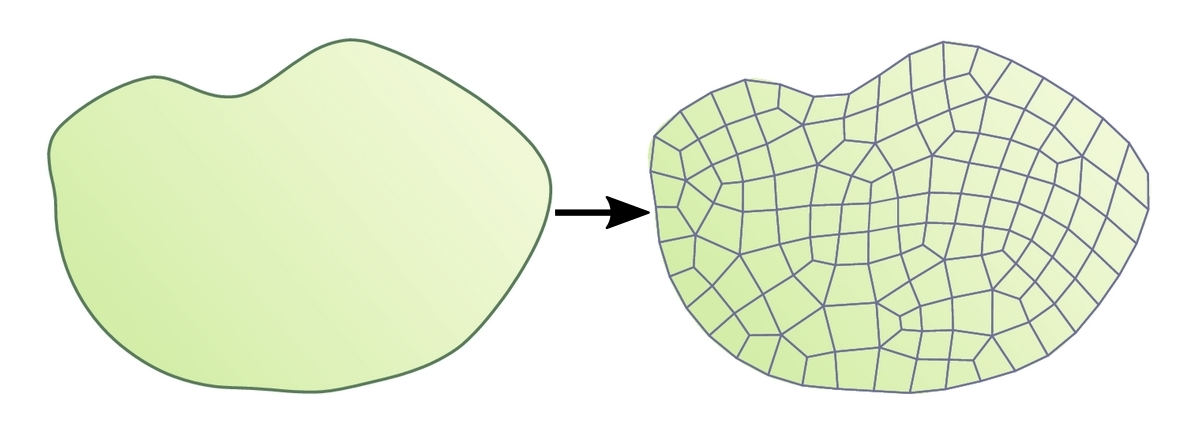
\includegraphics[scale=1.3]{figuras/dom.png}
  \label{fig:dom}
  \legend{Fonte: \cite{Theler2013b}}
\end{figure}

A análise por CFD envolve, geralmente, quatro etapas distintas:

\begin{itemize}
\item Geração da malha (ou preprocessamento): A partir da geometria do sistema, que equivale ao
  domínio contínuo, é necessário gerar uma malha. Essa malha pode ser refinada
  em pontos estratégicos, ser estruturada ou não-estruturada e possuir elementos
  de diferentes formatos. A malha utilizada na solução de um problema tem impacto
  direto no tempo de simulação, na qualidade da solução e até mesmo no alcance
  da solução. Em um projeto de CFD, aproximadamente 50\% do tempo é dedicado a geração
  da geometria e da malha \cite{Versteeg2007}.
\item Modelagem matemática: Equivale a definir, com base no conhecimento
  físico do problema, as hipóteses válidas, eventuais simplificações e
  seus impactos na solução final. A partir das definições, é necessário
  descrever as condições iniciais e de contorno de problema, as propriedades
  termo-físicas, químicas, fenômenos modelados e quaisquer outras características
  necessárias à solução do problema.
\item Solução: Nesta etapa são resolvidos os sistemas lineares obtidos pela
  discretização do domínio. Um dos métodos de discretização mais utilizados
  em problemas envolvendo comportamento de fluidos é o de volumes finitos. Além dos
  métodos de discretização, há diversos métodos para a solução dos sistemas
  lineares resultantes da discretização, com melhor ou pior desempenho de
  acordo com características do sistema linear a ser resolvido \cite{Barrett1994}.
\item Análise dos resultados (ou pós-processamento): Após a finalização
  com sucesso da simulação, os usuário deve tratar a grande quantidade de
  dados obtidos. Esta etapa consiste em extrair os resultados qualitativos
  e quantitativos, através do uso de ferramentas de visualização, estatística,
  matemáticas dentre outras \cite{Maric2014}.
\end{itemize}

Nos cálculos por CFD são resolvidas as equações fundamentais de transporte de massa (Equação \ref{eq:massa}),
momento (Equação \ref{eq:momento}) e energia (Equação \ref{eq:energia}), apresentadas abaixo em notação tensorial compacta \cite{dosSantos2012}.

\begin{equation}
%  \centering
  \label{eq:massa}
  \frac{\partial \rho}{\partial t}+\frac{\partial}{\partial x_j}(\rho u_j)=0
\end{equation}

\begin{equation}
%  \centering
  \label{eq:momento}
  \frac{\partial \rho u_i}{\partial t}+\frac{\partial}{\partial x_j}(\rho u_i u_j)=
  -\frac{\partial p}{\partial x_i} + \frac{\partial}{\partial x_j}\bigg[ \mu \bigg( \frac{\partial u_i}{\partial x_j} + \frac{\partial u_j}{\partial x_i}\bigg)\bigg]+S_{Mi}
\end{equation}

\begin{equation}
%  \centering
  \label{eq:energia}
  \frac{\partial \rho h_{tot}}{\partial t}-\frac{\partial \rho}{\partial t}+\frac{\partial}{\partial x_j}(\rho u_i h_{tot})=
  \frac{\partial p}{\partial x_j}\bigg( \lambda \frac{\partial T}{\partial x_i}\bigg) + \frac{\partial}{\partial x_j}\bigg[ u_i\mu \bigg( \frac{\partial u_i}{\partial x_j} + \frac{\partial u_j}{\partial x_i}\bigg)\bigg]+S_{E}
\end{equation}

Sendo $h_{tot} = h_{(T,p)} + \frac{u_i^{2}}{2}$ a entalpia total e $S_{Mi}$ e $S_E$, respectivamente, os termos
fonte das equações de momento e energia.

De acordo com a natureza do processo a ser simulado, alguns termos podem ser omitidos. Para o
caso de um cálculo estacionário, os termos relacionados à variações no tempo são
considerados nulos. Geralmente, tais simplificações levam consequentemente a
simplificações nos cálculos.

%Nesta seção serão apresentadas
%as equações utilizadas na modelagem de um sistema termo-hidráulico monofásico e
%estacionário.

% **********************************************
%\subsection{Equações governantes}
%\label{subsec:eq}


% **********************************************
%\subsubsection{Fluidos}
%\label{ssubsec:fluid}

% **********************************************
%\subsection{Turbulência}
%\label{subsec:turb}

%A modelagem da turbulência 
% **********************************************
%\subsection{Modelo termo-hidráulico discretizado}
%\label{subsec:modeloth}


% **********************************************
%\subsubsection{Sólidos}
%\label{ssubsec:solid}

% **********************************************
\section{Neutrônica}
\label{sec:neutronica}

Neutrônica pode ser definida como o estudo do movimento e interações dos nêutrons
com a matéria. O conhecimento de neutrônica é fundamental para determinar o
comportamento de um reator nuclear ou outros elementos que utilizem nêutrons
em feixes. A neutrônica é, em última instância, o estudo do transporte de nêutrons.

A probabilidade de interação entre um nêutron incidente e um núcleo alvo é caracterizada
pela seção de choque microscópica (unidade \textit{barn}, símbolo $\sigma$ e
equivalente a $10^{-24} cm^2$), que depende do núcleo alvo, do tipo de interação e da
energia do nêutron incidente. Essa dependência pode ser complicada devido a diversos fatores,
como a ordem de grandeza das energias envolvidas, levando a variações súbitas nas probabilidades
de interação. Estas variações são chamadas ressonâncias. A seção de choque macroscópica nada mais
é do que a seção de choque microscópica multiplicada pela densidade nuclear. Ela dá as probabilidades
médias de reação entre nêutrons de determinada energia com o material presente considerando a massa
do material. Sua unidade é dada em $cm^{-1}$.

%No escopo desta tese, é suficiente afirmar que as seções de choque são elementos fundamentais
%na descrição e, portanto, no cálculo neutrônico. 

% **********************************************
\subsection{Dados nucleares}
\label{subsec:dn}

% Do Hebért
A colisão entre um nêutron e um núcleo pode produzir reações nucleares de diferentes
tipos. Em um caso simples, o nêutron é simplesmente desviado, numa colisão elástica.
Em outros casos, esta interação pode produzir um núcleo composto, quando o nêutron é
absorvido pelo núcleo alvo. Neste caso, a energia do nêutron incidente é transmita para
o núcleo alvo que se torna instável. As formas de liberação dessa energia podem ser desde
a liberação de raios gama até a fissão deste núcleo.

O conceito de seção de choque \cite{Hebert2009} é usado para descrever a probabilidade
de cada tipo de reação nuclear e é baseado em propriedades fundamentais que caracterizam
as interações nucleares com os nêutrons.

A seção de choque microscópica ($\sigma_x$) é um fator de proporcionalidade numa relação entre
a taxa de reações numa determinada superfície e o número de nêutrons vezes a velocidade
relativa dos nêutrons em relação ao alvo e a densidade de nêutrons no feixe incidente.
Sua unidade é a unidade de superfície, data usualmente em $barns$ ($b=10^{-24}cm^2$).

A seção de choque macroscópica é definida a partir da seção de choque microscópica ($\Sigma_x$)
multiplicada pela densidade do material (que pode ou não ser composto por diferentes elementos ou
isótopos). É dada em $cm^{-1}$ e representa a chance efetiva de interação de um nêutron incidente
com todos os núcleos em um dado volume.

Fundamental para os cálculos neutrônicos, a obtenção de seções de choque representativas para
o sistema que se pretende calcular é usualmente feita a partir de bibliotecas de seções de choques
contínuas. Estas bibliotecas são utilizadas como entrada para códigos capazes de processar
as seções de choques contínuas, como o WIMS \cite{Halsall1986},
em bibliotecas de seções de choque isotópicas colapsadas em grupos.
Estas seções de choque processadas são então utilizadas tanto em cálculos por métodos
estocásticos quanto determinísticos.


% **********************************************
\subsection{Métodos estocásticos}
\label{subsec:mc}

Uma das formas de se modelar a interação de partículas, no presente caso nêutrons,
com a matéria, que por sua vez pode ser um fluido, gás ou sólido, é através de
métodos estocásticos (ou probabilísticos). As técnicas baseadas em números
aleatórios são chamadas de Monte Carlo devido ao famoso cassino com este nome
localizado em Mônaco.

As técnicas de Monte Carlo, ou especificamente chamado método de Monte Carlo
nas ciências nucleares, se baseiam na probabilidade de que determinados eventos,
quanto testados um número suficiente de vezes, possam ser representados
com acurácia por probabilidades

Na neutrônica, uma das formas de se representar o transporte
e colisões entre nêutrons é através do
uso do método de Monte Carlo \cite{Hutchinson2015}.

%Na Figura \ref{fig:random_walk}
%são mostradas algumas interações possíveis de um nêutron, desde seu surgimento
%até sua absorção.

%\begin{figure}[htb]
%  \caption{Exemplo de interações de um nêutron com a matéria.}
%  \centering\includegraphics[scale=0.5]{figuras/random_walk.png}
%  \label{fig:random_walk}
%  \legend{Fonte: autor}
%\end{figure}

O objetivo principal das simulações por Monte Carlo é, geralmente, determinar
o valor médio de algum parâmetro relativo ao comportamento das partículas simuladas, como o fluxo de
nêutrons em função de sua posição, por exemplo. Cabe lembrar que, por depender
de um grande número de eventos para ser estatisticamente válida, uma única
simulação por Monte Carlo pode extremamente custosa do ponto de vista computacional.
Ainda assim, o método é cada vez mais utilizado e, com o aumento de poder
computacional atual, mais viável para problemas complexos.

Uma breve introdução às técnicas de Monte Carlo, com ênfase no uso para
transporte de radiação e em nível de estudantes, pode ser encontrado
no livro de Hutchinson \cite{Hutchinson2015}.

% Falar de random walk
% Colisão e o que acontece
% Iteração com outras partículas
% Tracking e talling
% Incerteza

% **********************************************
\subsection{Métodos determinísticos: a aproximação por difusão}
\label{subsec:det}

A assim chamada aproximação por difusão é usualmente utilizada para cálculos
do fluxo neutrônico no núcleo de reatores, normalmente utilizando a teoria
de difusão para poucos grupos de nêutrons \cite{Hebert2009}.

A equação de difusão é obtida pela substituição da Lei de Fick na equação de
transporte integrada em todo o volume de cálculo, além de assumir
diversas simplificações \cite{Theler2013b}. A Lei de Fick funciona como
uma relação heurística entre entre o fluxo e a corrente de nêutrons.
Esta relação, entretanto, impõe algumas limitações nos problemas a serem
resolvidos. A Lei de Fick não é válida próxima a regiões
de descontinuidade, na proximidade de pontos de fuga ou termos-fonte, quanto
a anisotropia é suficientemente alta (quando a seção de choque
de absorção e da mesma ordem de grandeza da seção de choque total), em
meios altamente absorvedores, na proximidade de interfaces e quando há variação
rápida do fluxo (não é o caso em casos estacionários).
Algumas destas limitações, porém, podem ser corrigidas
em vários casos. A equação da difusão consiste
num conjunto de equações diferenciais parciais de segunda ordem resolvidas
em coordenadas espaciais.

A equação de difusão para multi-grupos é dada pela equação \ref{eq:dif} \cite{Demaziere2014}:

\begin{equation}
  \label{eq:dif}
  %    \begin{split}
  -\nabla.[D_g(\mathbf{r})]\nabla \phi_g(\mathbf{r})+ \Sigma_{(T,g)}(\mathbf{r})\phi_g(\mathbf{r}) =
  \sum_{g'=1}^{G} \Sigma_{s0,g'\rightarrow g}(\mathbf{r})\phi_{g'}(\mathbf{r}) +
  \frac{\chi_g}{k}\sum_{g'=1}^{G}\nu_{g'}\Sigma_{f,g'}(\mathbf{r})\phi_{g'}(\mathbf{r})
  %\end{split}
\end{equation}

% Tabelar os termos

A equação de difusão pode ser resolvida analiticamente para casos simples, em geral em
casos didáticos, ou utilizando técnicas padrão de análise numérica, como o método de
elementos finitos ou volumes finitos.

Apesar de aparentemente grosseira devido às simplificações para sua obtenção, a equação
de difusão dá resultados próximos aos obtidos por métodos mais elaborados \cite{Theler2013b}.

É importante ressaltar que a Equação \ref{eq:dif} é um problema de \textit{autovalor}, cuja
solução existe para distintos autovalores $k$. O maior autovalor absoluto corresponde à
solução fundamental do problema de autovalor e é igual ao fator de multiplicação
efetivo ($k_{eff}$) do reator. Apenas a solução fundamental tem significado físico.

A compacta apresentação dada neste texto para as equações de Navier-Stokes e para a
equação de difusão visa apenas introduzir
as bases fundamentais dos problemas que são resolvidos pelos sistemas acoplados nesta tese.

% **********************************************
%\subsubsection{Equação de Transporte}
%\label{ssubsec:transp}

% **********************************************
% \subsubsection{Aproximação por Difusão}
% \label{ssubsec:difusao}

% **********************************************
%\subsection{Modelo neutrônico discretizado}
%\label{subsec:modelon}



% ----------------------------------------------------------
% Metodologia
% ----------------------------------------------------------
% ----------------------------------------------------------
% Metodologia
% ----------------------------------------------------------
\chapter{Metodologia}
\label{chap:metodologia}

O trabalho de tese em questão trata do desenvolvimento e teste
de um sistema de \textit{software}. Desse modo, a metodologia utilizada no desenvolvimento
deste sistema e, portanto, na solução do problema proposto,
é construída com base nos seguintes aspectos:

\begin{itemize}
\item Adequação das ferramentas utilizadas para alcançar o objetivo de um sistema de cálculos acoplados;
\item As restrições impostas pelas ferramentas escolhidas devido à sua estrutura intrínseca.
\end{itemize}

Desse modo, é desejável, do ponto de vista de clareza, descrever a metodologia utilizada no trabalho
apresentando as características das ferramentas utilizadas, suas limitações e seus possíveis impactos
no resultado final, de modo a então descrever a solução acoplada. Por sua vez, na descrição da solução
acoplada, são apresentadas as modificações implementadas nas ferramentas e as formas de utilização
de dois programas de computador independentes de forma conjunta.


\section{Visão Geral}

O sistema de \textit{software} desenvolvido tem algumas peculiaridades relativas à sua
implementação. Isso se deve às particularidades do problema que se pretende resolver e ao
fato não-usual de envolver duas peças de \textit{software} independentes para resolver
um problema complexo, já apresentado como um problema multi-física.

A Figura \ref{metodoetapas} apresenta uma representação gráfica do funcionamento do sistema
acoplado desenvolvido.

\begin{figure}[htb]
  \caption{Metodologia: o sistema acoplado.}
  \centering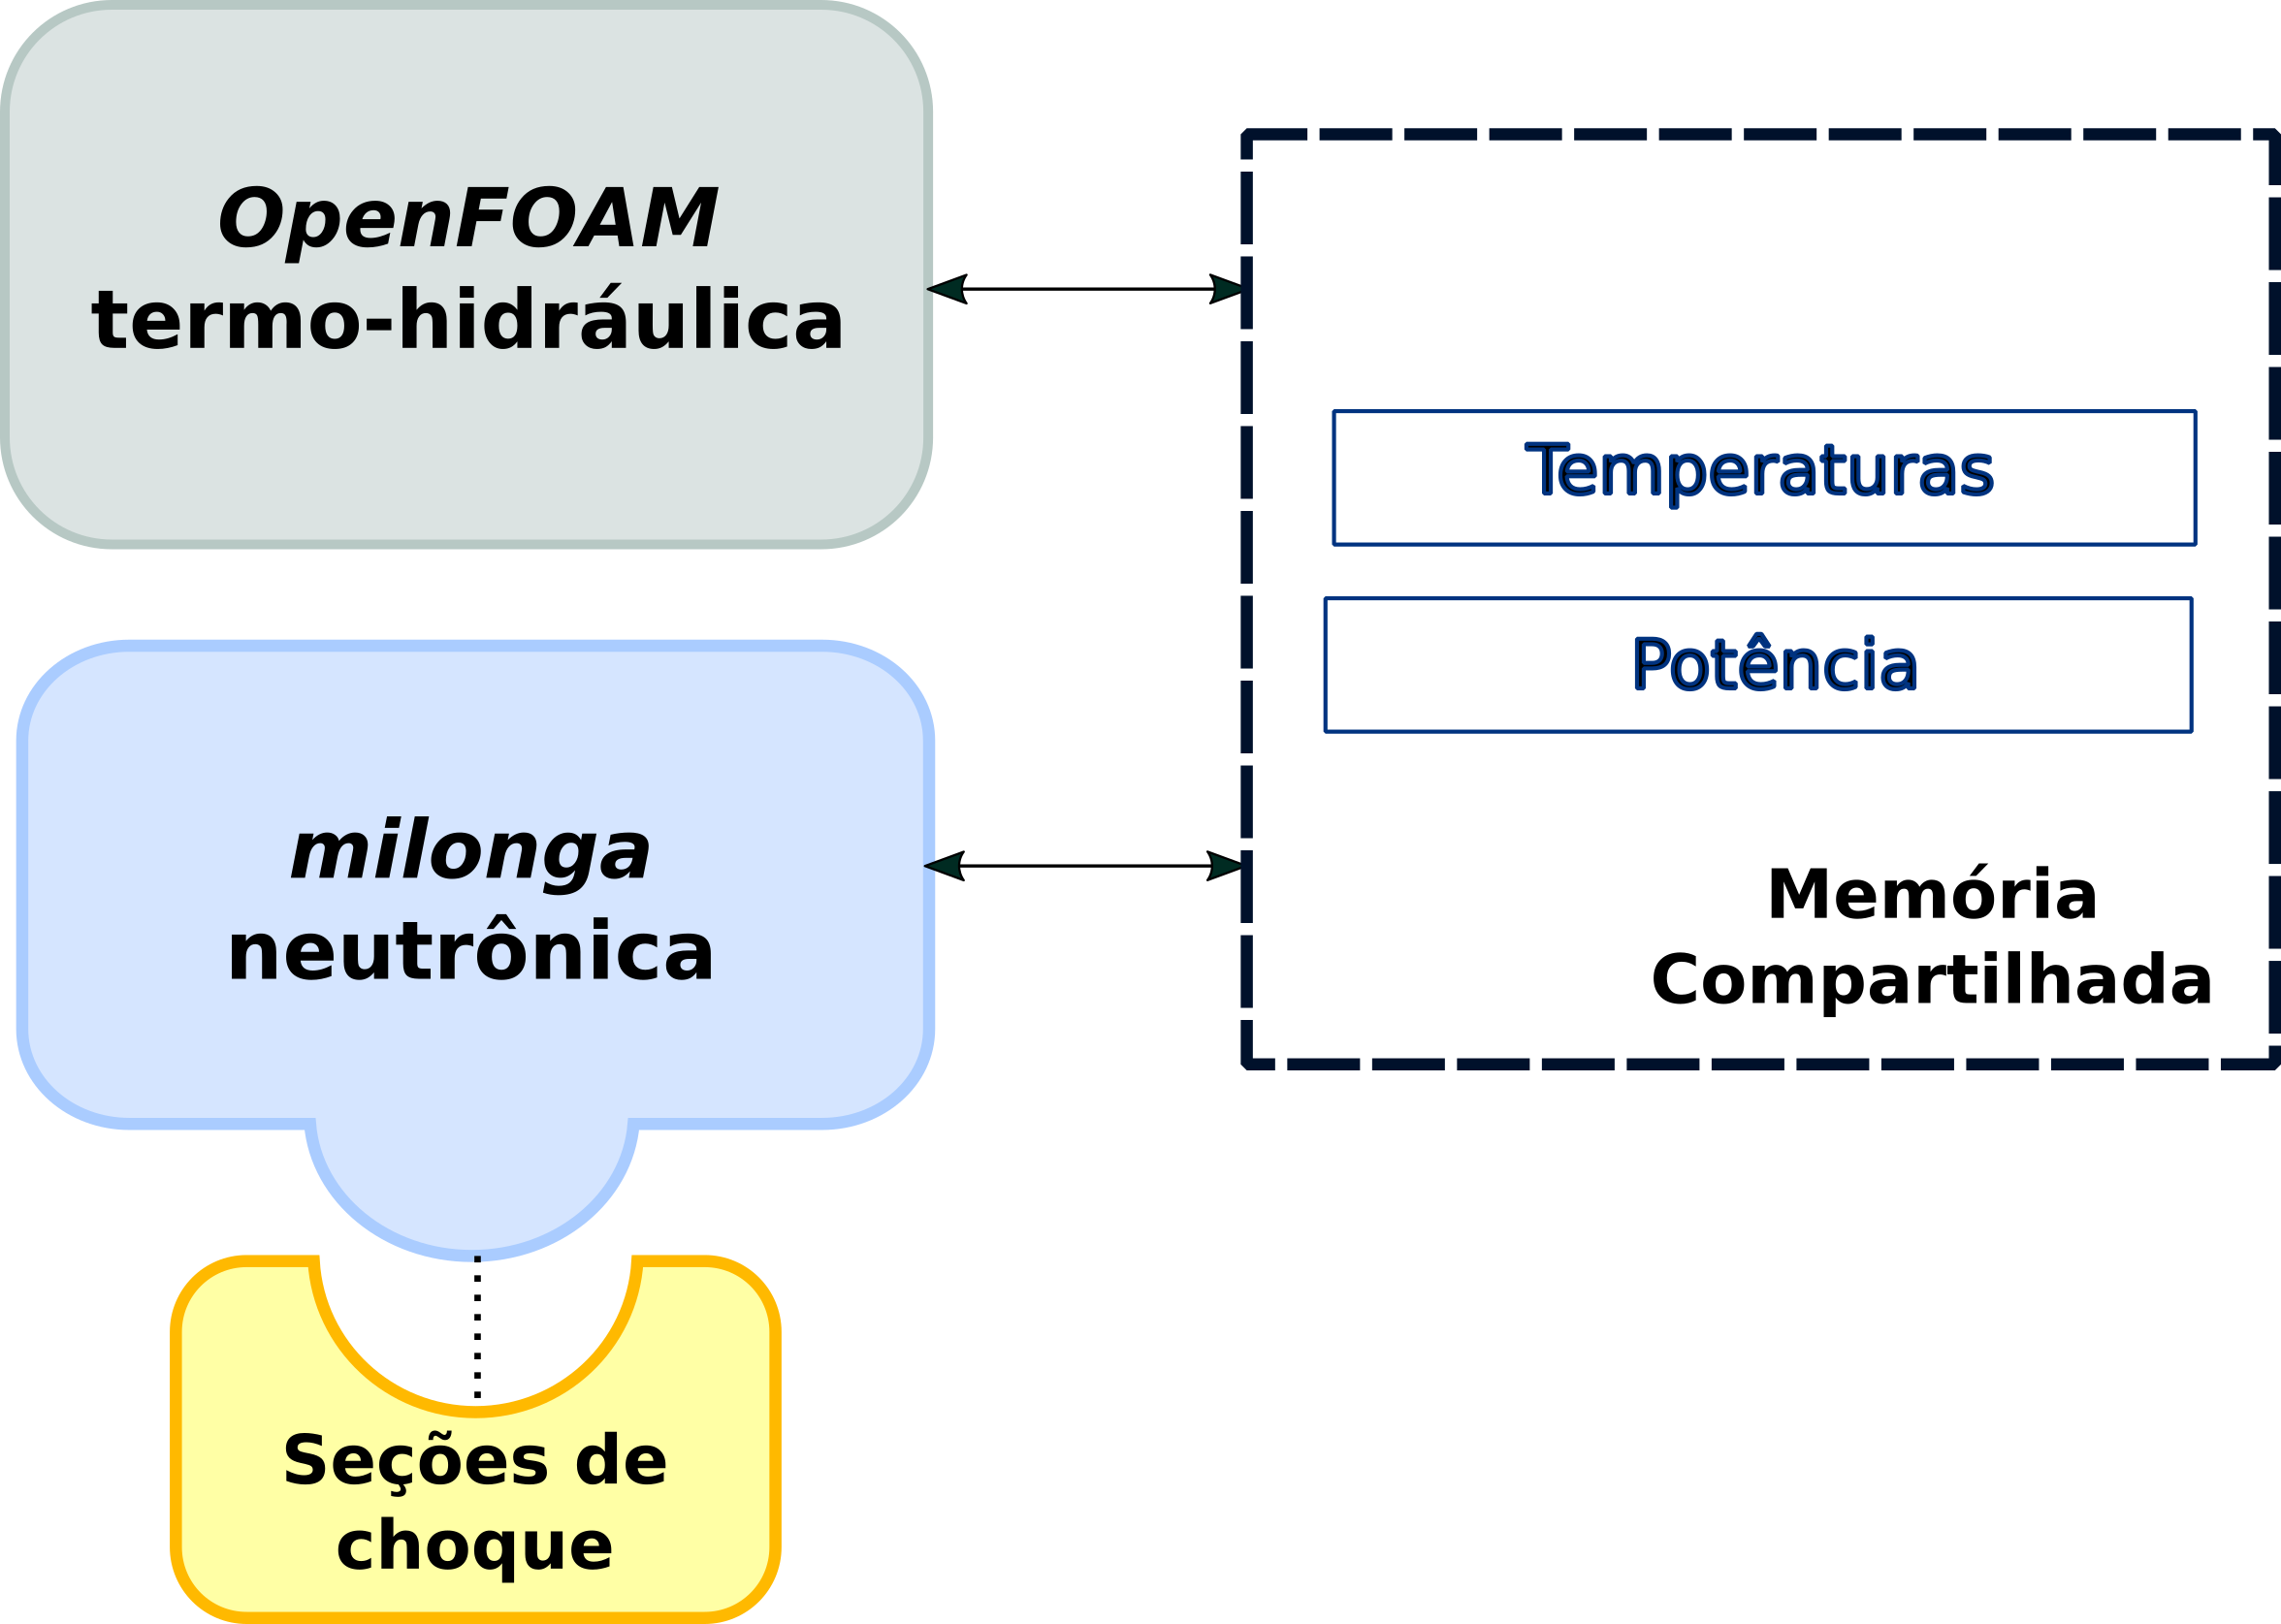
\includegraphics[scale=0.6]{figuras/metodologia2.png}
  \label{metodoetapas}
%  \legend{Fonte: autor}
\end{figure}

Como apresentado no capítulo \ref{chap:rev}, acoplamento, no contexto desta dessa tese, é a execução
de cálculos termo-hidráulicos utilizando a potência obtida pelo código de neutrônica que, por sua vez,
utiliza as temperaturas dos materiais calculadas pela termo-hidráulica para re-calcular seções de choque
e outros parâmetros neutrônicos de modo a calcular o fluxo de nêutrons e potência no combustível.

As características não-usuais desse sistema são listadas abaixo:

\begin{itemize}
\item Dois \textit{softwares} independentes interligados;
\item Uso de memória compartilhada para comunicação entre dois diferentes códigos;
\item Natureza aberta das licenças de utilização de ambos os programas (item fundamental para
  o acesso, modificação e utilização do código-fonte de ambos);
  \item Uso da mesma malha por ambos os códigos.
\end{itemize}

Nas próximas seções serão apresentadas em seus detalhes cada uma destas características que
permitiram o desenvolvimento de um sistema multi-física.

\section{Conceitos}
\label{sec:conc}

O sistema acoplado, ou multi-física, apresentado nesta tese possui algumas características
particulares já citadas. Nesta seção, serão brevemente apresentados os conceitos sobre os quais
foi possível desenhar e construir um sistema multi-física inovador com tais características.

\subsection{Multi-tarefa}
\label{subsec:mt}

Multi-tarefa é a capacidade dos sistemas operacionais de executar distintas tarefas ao mesmo tempo.
Talvez possa parecer corriqueira tal observação nos dias de hoje. Entretanto, há pouco mais de vinte
anos, a maioria dos sistemas operacionais usados em computadores pessoais não ofereciam esta
possibilidade. Em alguns casos, o que se chamou de multi-tarefa preemptiva, o usuário era capaz de
carregas distintas tarefas em memória. Contudo, apenas uma era executada por vez.

Nos sistemas computacionais atuais, em especial no sistema Linux, utilizado para o desenvolvimento
do sistema multi-física desta tese, é possível executar diversas tarefas ao mesmo tempo. Não só isso,
como há um sistema padrão de execução que permite a comunicação entre programas distintos. Diferente
de um sistema de \textit{threads} \cite{Walli1995},
em que todos os programas lançados enxergam a mesma
porção de memória, no sistema Linux cada programa tem acesso exclusivo à memória alocada para si.
Tudo isso acontece sob gerenciamento do sistema operacional.

A metodologia utilizada neste acoplamento, prevê a execução separada dos programas de termo-hidráulica
e neutrônica. Os detalhes e os algoritmos desta comunicação serão apresentados em detalhes oportunamente.
Por agora, é suficiente saber que os programas são lançados separadamente, cada qual utilizando a memória
alocada para si separadamente, sem que outros programas possam acessá-la. Dessa forma, era necessário
desenvolver um sistema ou forma de comunicação entre os códigos de neutrônica e termo-hidráulica.

\subsection{Memória compartilhada}
\label{subsec:mc}

Memória compartilhada (ou \textit{Shared-memory}) é a memória de computadores que pode ser
acessada simultaneamente por múltiplos programas em executados em diferentes
espaços de usuários com o objetivo de oferecer comunicação entre
eles evitando cópias redundantes \cite{Robbins2003}. É, ainda, uma forma eficiente
de troca de dados entre programas ou processos. A interface POSIX
(\textit{Portable Operating System Interface}) \cite{Walli1995} é um
padrão especificado pela \textit{IEEE Computer Society} para garantir
a compatibilidade entre diferentes sistemas operacionais na implementação
das formas de utilização da memória compartilhada. Para isso, é definida
uma API (\textit{Application programming interface}) que explicita as funções
e métodos de utilização da memória compartilhada. O padrão e a API disponibilizada
garatem a compatibilidade no uso dos recursos entre diferentes programas ou \textit{threads}
\cite{Atlidakis2016}.

Com mais de um programa acessando uma mesma área de memória, é necessário garantir a atomicidade
das operações por cada programa. Por atomicidade, entenda-se que uma operação iniciada por um
programa ou \textit{thread} deve ser completamente encerrada antes que outro programa ou
\textit{thread} acesse esta memória. À possibilidade de acesso concorrente ao mesmo recurso
de memória, dá-se o nome de condição de corrida.

Há diferentes técnicas para evitar condições do corrida. Dentre elas, uma das mais simples e
largamente empregada, é o uso de semáforos, inclusive usada nesta tese.
Um programa ou \textit{thread}, antes de acessar a memória
verifica se esta está livre para ser acessada. Se sim, altera o valor do semáforo enquanto opera na
memória, voltando a alterá-lo para ``livre'' ao terminar. Caso outro programa ou \textit{thread}
necessite acessar a mesma porção de memória, encontrará o semáforo em condição negativa e aguardará
um determinado tempo (definido pelo sistema operacional ou pelo próprio usuário) até tentar novamente.
Com isso, fica garantida a não-corrupção dos dados.

Deve-se dizer que há implicações negativas no uso de semáforos para controle de acesso à memória,
como por exemplo, queda de desempenho dos sistemas, em especial quando há um número grande
de programas acessando a memória compartilhada. Entretanto, a análise da possível degradação
de desempenho causada por controle de concorrência entre programas não é escopo desta tese.

\subsection{\textit{Software} livre}
\label{subsec:sl}

Muito já se disse sobre \textit{software} livre, suas características e suas licenças, como na
seção \ref{sec:intsl}. Nesta sub-seção, o objetivo se restringe às vantagens do acesso ao
código-fonte.

Ambos os códigos usados no sistema acoplado, possuem a capacidade de serem acoplados sem alterações
em seus códigos-fonte. O \textit{milonga}, em especial, já foi desenvolvido com a possibilidade
de acoplamento em mente. Portanto, oferece mais de uma forma de comunicação de dados, como por exemplo:
arquivos texto, arquivos binários e, inclusive, de forma nativa, uso de memória compartilhada.

O \textit{OpenFOAM}, entretanto, em um cenário de código fechado, só ofereceria uma forma de
acoplamento. De acordo com sua implementação, um termo-fonte só pode ser lido a cada início de
simulação. Seria, portanto necessário fazer com que o \textit{mionga} lesse os dados de temperatura
da saída do \textit{OpenFOAM}, escrevesse uma distribuição de potências em formato de entrada
para o \textit{OpenFOAM} e que este fosse novamente executado do zero. Todo esse processo, deveria
ser controlado por um \textit{script} de execução.

Apesar de soar rudimentar, está é a forma de acoplamento mais comumente empregada.
Mesmo com severo comprometimento de desempenho se comparada ao compartilhamento de
memória, técnica usada nesta tese, muitas vezes essa é a única forma de acoplamento
quando o código-fonte não está disponível \cite{Hummel2016}.

\subsection{Discretização do domínio}
\label{subsec:dd}

A formulação utilizada para a solução da equações diferenciais que modelam o problema multi-física desta
tese é a de volumes finitos. Uma característica básica desta técnica é a utilização de pequenos volumes
de modo que as equações diferencias possam ser resolvidas como equações algébricas. A forma de obtenção
destes pequenos volumes a partir de um domínio contínuo é o que se chama \textbf{discretização de domínio}. 

A discretização do domínio significa, na prática, gerar uma malha que represente o domínio contínuo original
mantendo a conexão entre os pequenos volumes gerados. Se o domínio for tridimensional, será, geralmente,
discretizado por uma malha volumétrica. Um dos diferenciais do acoplamento apresentado está exatamente na
utilização da mesma malha para os cálculos neutrônicos, realizados pelo \textit{milonga} e termo-hidráulicos,
realizados pelo \textit{solver OpenFOAM}. Com ambos os programas utilizando a mesma malha, a relação é de um
pra um. Uma célula na neutrônica é representada exatamente pela mesma célula na termo-hidráulica.

Como mencionado anteriormente, a utilização da mesma malha para neutrônica e
termo-hidráulica é uma característica
particular do acoplamento proposto. São raros os acoplamentos com essa característica
encontrados na literatura \cite{Jareteg2014} e suas vantagens são, principalmente:

\begin{itemize}
\item Solução multi-física no mesmo nível de detalhes\footnote{Neste trabalho, se considera ``nível de detalhes'' o
  mesmo grau de discretização para ambos os problemas. O conceito pode ser estendido se for
  considerado o erro relativo dos cálculos em cada problema. Não é este o caso.};
\item Evita-se o mapeamento entre malhas que, no caso de malhas não-estruturadas, além de ser um problema de
  geometria computacional não-trivial , eventuais soluções podem acrescentar
  erros entre células \cite{Kraevoy2004}.
\end{itemize}

\subsection{Limitações}
\label{subsec:lim}

O sistema multi-física construído tem limitações, principalmente devido à limitação intrínseca de um ou de ambos
os programas usados no acoplamento. As restrições, como foram assim chamadas no início do capítulo
\ref{chap:metodologia}, são apresentadas
em forma de lista:

\begin{itemize}
\item \textbf{Sistema Operacional}: Ambos \textit{OpenFOAM} e \textit{milonga}, apesar de livremente disponíveis e,
  portanto, passíveis de utilização em diferentes sistemas operacionais são fornecidos especificamente
  para sistemas Linux. Alguns esforços recentes mostram eventuais aplicações do primeiro em sistemas
  Windows. Já para o \textit{milonga}, não há qualquer previsão de uso em outros sistemas operacionais;
\item \textbf{Execução em Paralelo}: O \textit{OpenFOAM} oferece de forma nativa a possibilidade de execução em
  paralelo. O \textit{solver} \texttt{thesisCoupledFoam} foi, inclusive, implementado de modo a funcionar em paralelo.
  Entretanto, dada a limitação do \textit{milonga}, até sua versão 0.4.65, em executar em paralelo, o sistema
  de comunicação do acoplamento está limitado a execução sequencial.
\item \textbf{Seções de choque}: a geração de seções de choque deve ser feita por algum código externo. Os
  principais códigos empregados para geração de seções de choque são fechados ou, como no
  caso do \textit{Serpent} aberto mas restrito. Entretanto, neste campo também há uma recente
  atividade no que diz respeito a \textit{software} livre. O conjunto de ferramentas \textit{PyNE},
  oferecido sob licença BSD (aberto e gratuito), tem como uma de suas propostas, a geração de seções
  de choque para aplicações de ciências nucleares e engenharia nuclear \cite{Slaybaugh20014}.:
\item \textbf{Memória}: O \textit{milonga} oferece, além da formulação de solução pela equação de difusão,
  algumas variações do método de ordenadas discretas. Entretanto, o consumo de memória e tempo de execução
  nestas formulações foi proibitivo no \textit{hardware} disponível no momento de desenvolvimento desta tese.
\end{itemize}

Apresentadas as limitações, cabe ressaltar que tais limitações, apesar de implicarem no uso,
execução e até na qualidade dos resultados dos cálculos, não são definitivas.
A quase totalidade das limitações e restrições apresentadas na lista
acima podem ser resolvidas com moderado investimento de tempo. Especificamente, tempo empregado em implementação
de novas funcionalidades como, por exemplo, a execução em paralelo do código de neutrônica ou a compilação
das ferramentas para outro sistema operacional.

Isto posto, é possível perceber que no mundo do \textit{software} limitações podem ser temporárias, de modo que um
conceito bem estabelecido pode passar antes do que se imagina, a uma ferramenta de utilização ampla.

\section{Ferramentas}
\label{sec:ferr}

Na seção anterior, foram brevemente descritos os conceitos sobre os quais foi construído
o sistema acoplado desenvolvido nesta tese. Este
sistema utiliza dois diferentes programas de computador. Cada um deles
realiza um conjunto de cálculos separadamente e compartilham os dados necessários aos cálculos do outro.

Apesar de desenvolvidos separadamente e com objetivos diferentes, algumas características comuns - além
do fato de serem ambos \textit{software} livre - permitiram seu uso acoplado. Ambos possuem a capacidade de lidar
com um mesmo formato aberto de arquivos de descrição de malhas, por exemplo.

%São dedicadas subseções a cada característica deste acoplamento definida anteriormente como não-usual.

As próximas sub-seções exploram as características destes programas que permitiram desenvolver
a metodologia neste acoplamento. São também apresentados os principais desenvolvimentos técnicos
relacionados a metodologia desenvolvida.

\subsection{Termo-hidráulica: \textbf{OpenFOAM}}
\label{subsection:openfoam}

O \textit{OpenFOAM} é um pacote para simulação numérica de Mecânica
do contínuo desenvolvido com base em orientação a objetos em linguagem $C++$ .
Do ponto de vista de Engenharia de Software, sua modularidade e flexibilidade são vantagens
em relação a outros códigos monolíticos  \cite{Jasak2007}. Sua implementação em componentes para manipulação de malhas, suporte
à solução de sistemas lineares, operadores de discretização e modelos físicos em forma de bibliotecas o tornam
um sistema CFD completo, aberto e gratuito. É utilizado em uma grande variedade
de aplicações, desde a solução de escoamentos complexos envolvendo reações químicas, turbulência e
transferência de calor até acústica, mecânica dos sólidos e eletromagnetismo. 

\textit{OpenFOAM} implementa um manipulador de malhas poliédrico, no qual células são descritas a partir
de um conjunto de faces fechando um volume. As faces, por sua vez, são formadas por uma lista de pontos
em suas coordenadas cartesianas e armazenados como vetores. Esta implementação é independente da discretização
usada \cite{Jasak2009}. Entretanto, as principais classes que herdam as funcionalidades das malhas implementam o método de
volumes finitos. Sendo assim, pode-se dizer que o \textit{OpenFOAM} é um sistema de CFD baseado em volumes
finitos.

Além dos componentes dedicados a operações sobre o domínio, o \textit{OpenFOAM} oferece um conjunto variado
de programas independentes chamados \textit{solvers}. Estes \textit{solvers} são dedicados à solução de
problemas físicos específicos. Para isto, utilizam outros elementos disponíveis no conjunto do
\textit{OpenFOAM}. O problema físico a ser resolvido nesta tese, especificamente do ponto de vista
termo-hidráulico, é o da solução de troca de calor conjugada entre sólidos e
fluidos distintos. Um dos \textit{solvers} que o \textit{OpenFOAM} possui com esse propósito é o
\texttt{chtMultiRegionSimpleFoam} \cite{OpenFOAM2015}.

Este \textit{solver} funciona para problemas em estado estacionário e para
fluidos compressíveis. A modularidade do \textit{OpenFOAM}
fica clara na forma como o \textit{solver} interage com os outros módulos: para regiões sólidas,
são utilizados modulos de propriedades termo-físicas específicos para sólidos. Por sua vez, para
fluidos são oferecidos outros módulos com implementações relativas a propriedades de fluidos.
Outro exemplo é a utilização de turbulência: caso o usuário estabeleça que seu escoamento é laminar,
o módulo para escoamentos laminares é utilizado. Caso o escoamento seja turbulento, o usuário pode
escolher entre implementações de diferentes modelos de turbulência.

O \textit{solver} utilizado permite escolher entre energia interna e entalpia para a solução
da equação da energia, de acordo com o módulo termodinâmico escolhido. Na implementação do
problema acoplado, foi usada entalpia. O modelo de turbulência utilizado foi o $\kappa-\epsilon$
\cite{Launder1974}.

%Mais detalhes as características do escoamento simulado e do modelo de turbulência serão
%discutidos no capítulo \ref{chap:aplicacao} e sub-seção \ref{subsec:turb}, respectivamente.

O \textit{OpenFOAM} é capaz de importar malhas no formato aberto \textbf{gmsh} \cite{Geuzane2009}. Este
formato é o mesmo utilizado pelo \textit{milonga} para leitura de malhas não-estruturadas.



% -----------------------------------------------------------------------------------------------------

\subsection{Neutrônica: \textbf{milonga}}
\label{subs:milonga}

O \textit{milonga} é um \textit{software} aberto e livre para cálculo de física de reatores
liberado sob licença to tipo GNU \cite{gplv3}. Ele é construído utilizando-se de bibliotecas
conhecidas como a \textit{GNU Scientific Library} \cite{Galassi2009}, a biblioteca
PETSc \cite{Balay2016} e na biblioteca para solução de problemas da autovalores e autovetores
SLEPc \cite{Hernandez2005}. A re-utilização de bibliotecas consagradas traz robustez para
o \textit{milonga} enquanto segue os princípios do desenvolvimento de \textit{software} livre.

O \textit{milonga} resolve a equação de transporte de nêutrons multi-grupos em estado estacionário,
utilizando a aproximação por difusão ou o método de ordenadas discretas. Oferece dois esquemas
de discretização, elementos e volumes finitos. A capacidade de utilizar volumes finitos em malhas
não-estruturadas permite sua utilização de forma acoplada com o \textit{ÒpenFOAM}. O formato
de leitura de malhas não-estruturados utilizado pelo \textit{milonga} é o \textbf{gmsh}, formato
este que o \textit{OpenFOAM} é capaz de importar, como mencionado anteriormente.

Dentre as distintas formas de resolver a equação de transporte oferecidas pelo \textit{milonga},
optou-se por utilizar a aproximação por difusão. Apesar de resultados inacurados e das limitações
na sua utilização em algumas circunstâncias \cite{Trahan2014}, a aproximação por difusão
foi o modelo escolhido devido à sua execução mais rápida e menor consumo de memória.
A aproximação por difusão é apresentada na equação \ref{eq:difusao} já na sua forma discretizada
para $G$ grupos:

\begin{equation}
  \label{eq:difusao}
  \begin{split}
  & 0 = \nabla . \big[D_g({\bar{x}}) \nabla \phi_g(\bar{x})\big] 
- \Sigma_{tg}(\bar{x}).\phi(\bar{x}) \\
& + \sum_{g'=1}^{G} \Sigma_{sg'\rightarrow g}(\bar{x}) . \phi_{g'}(\bar{x})
+ \chi(g)  \sum_{g'=1}^{G} \frac{\nu \Sigma_{fg'}(\bar{x})}{k_{eff}} . \phi_{g'}(\bar{x}) \\
  \end{split}
  \end{equation}

(Inserir a tabela de grandezas)

A dependência das seções de choque da temperatura pode ser considerada linear uma vez que
os coeficientes são mantidos constantes durantes cada passo do cálculo iterativo utilizado
pelo \textit{milonga}

De forma padrão, o \textit{milonga} funciona lendo um arquivo de entrada que modela o
problema a ser resolvido. Um dos casos mais simples em que se resolve o fluxo de nêutrons
num sistema crítico, com seções de choque constantes, é apresentado na figura \ref{fig:inputmilonga}.
Além dos comandos apresentados, o \textit{milonga} possui um vasto conjunto de comandos e primitivas
que vão desde pré-processamento da malha até primitivas de saída para visualização gráfica da
solução.

\begin{figure}[htb]
  \caption{Arquivo de entrada básico do milonga. A definição da formulação,
    esquema de solução e número de grupos é apresentada na linha 7. Os coeficientes
    da equação de difusão para um material são apresentadas nas linhas 10-16.
    Condições de contorno baseadas na malha estão definidas nas linhas 19-21 e na linha 24
  está o comando utilizado para iniciar os cálculos.}
  \centering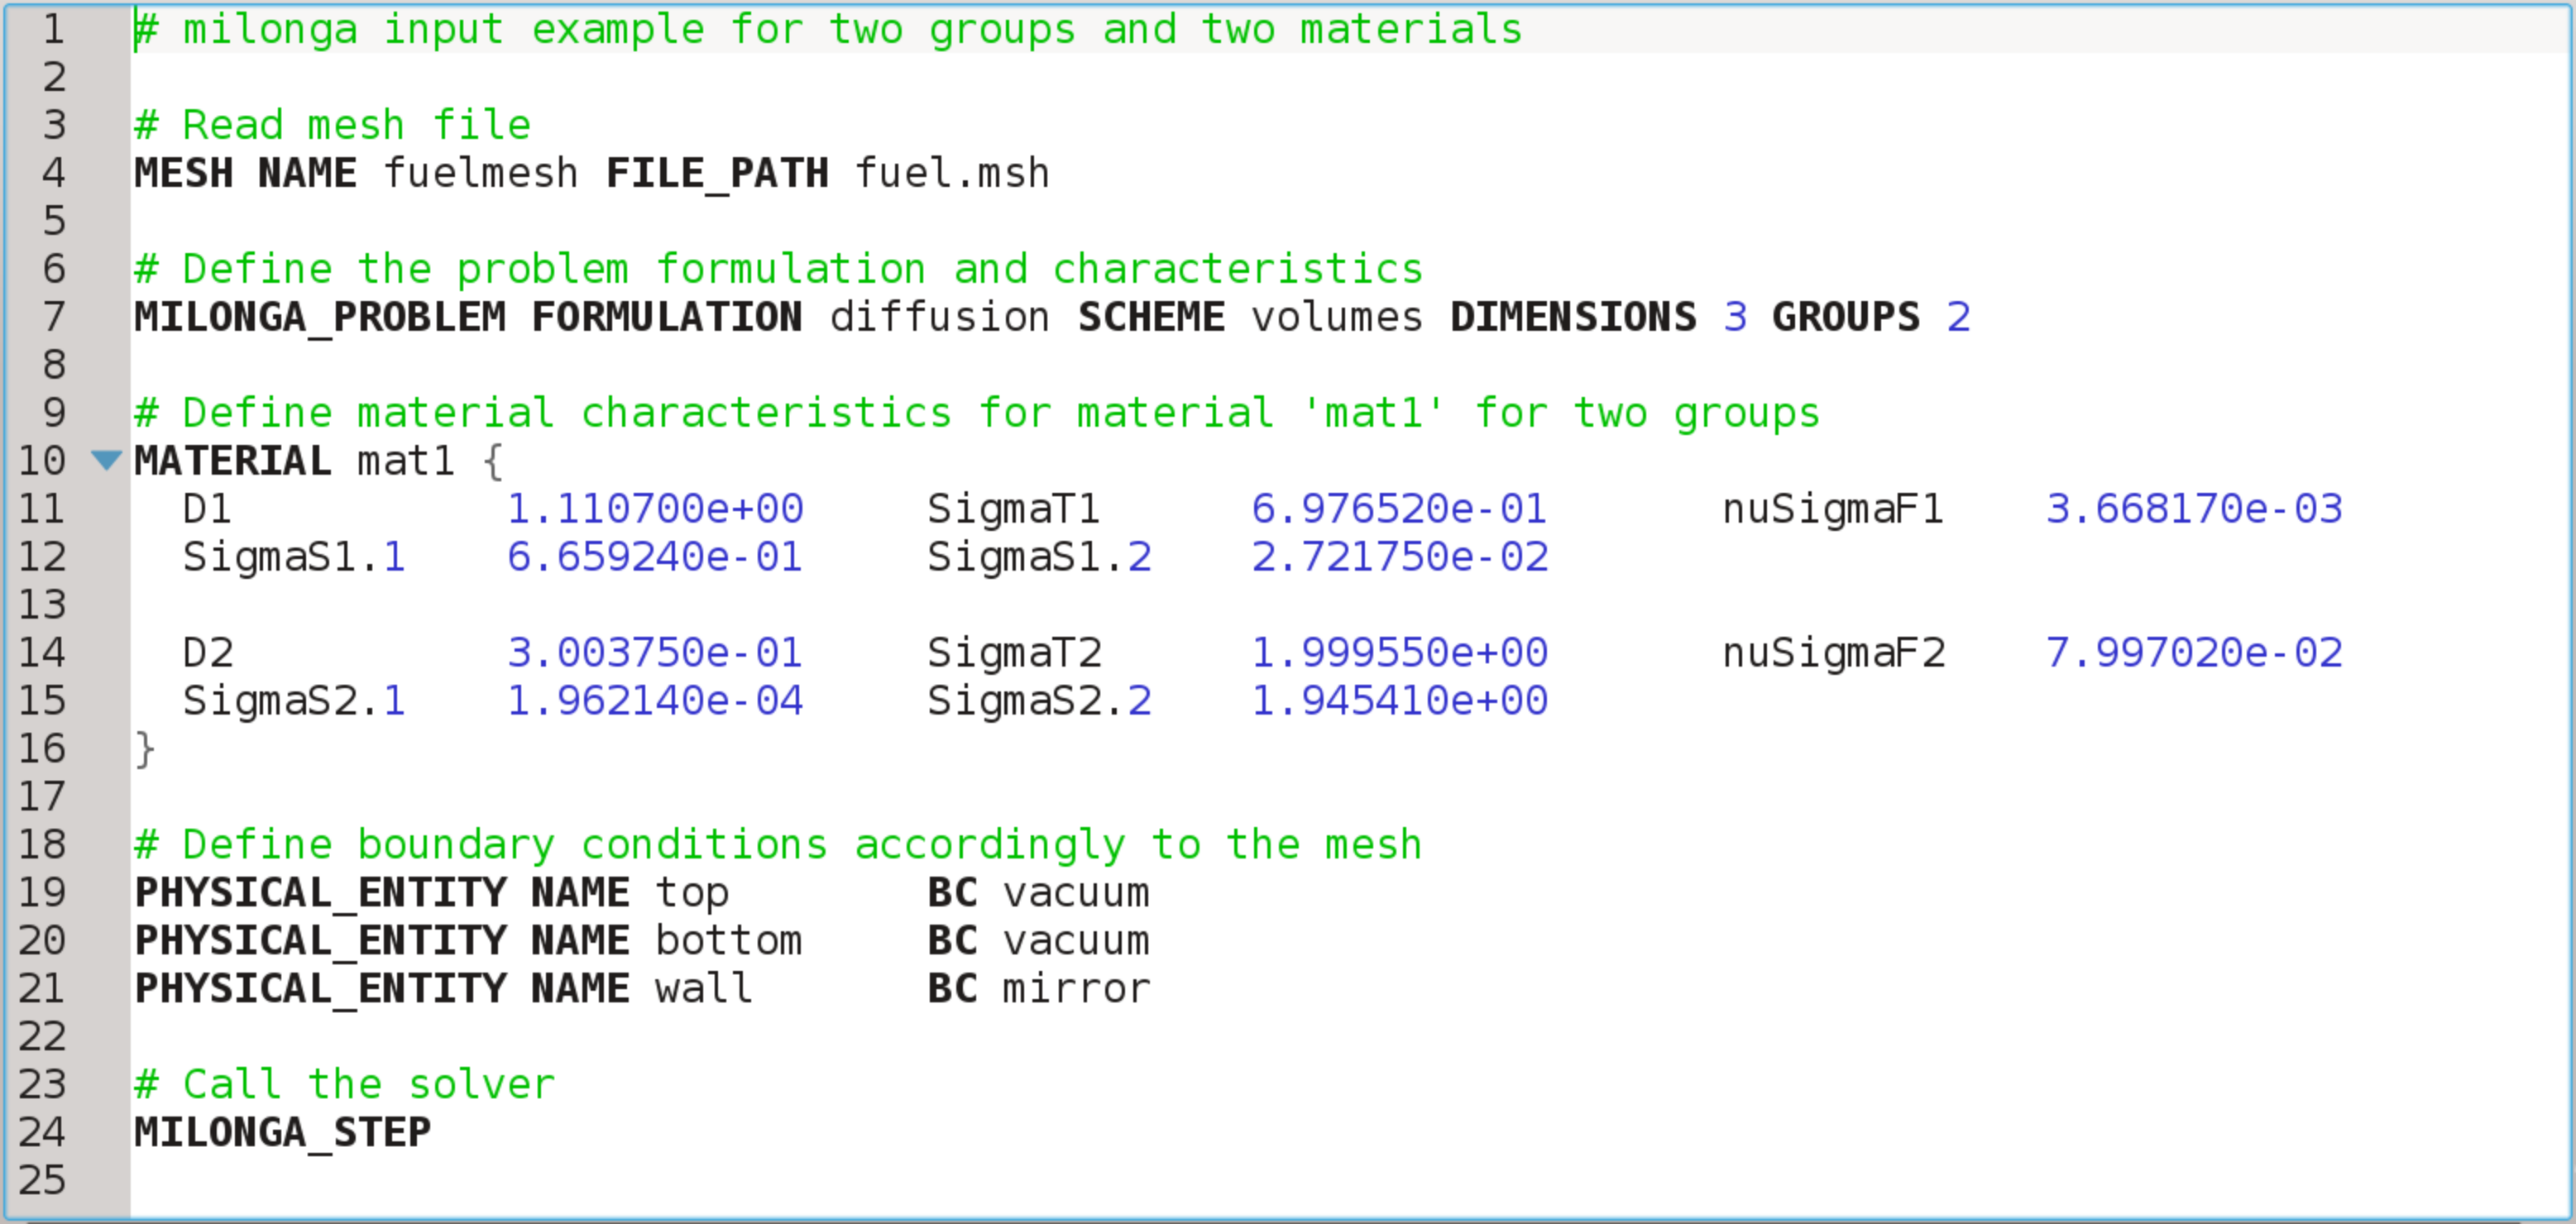
\includegraphics[scale=0.19]{figuras/milonga_example2.png}
  \label{fig:inputmilonga}
%  \legend{Fonte: autor}
\end{figure}

Uma funcionalidade fundamental do \textit{milonga} para o acoplamento neutrônico
e termo-hidráulico é a possibilidade de definir as seções de choque como expressões
algébricas de $x$, $y$ e $z$, como funções definidas geometricamente em $x$, $y$ e $z$
ou como combinação de ambos os métodos. Para o acoplamento, em especial, a definição
de funções geometricamente permite estabelecer valores para os coeficientes de
acordo com a posição da célula na malha. A aplicação é ainda mais extensa, já que
uma vez que é possível utilizar expressões pela posição na malha, é também
possível definir concetração de veneno ou fração de vazio por elemento da malha.

Além disso, o \textit{milonga} pode ser dados em tempo de execução de arquivos de
entrada, arquivos binários e, em especial no contexto desta tese, de memória compartilhada.
Esta é uma funcionalidade deste \textit{software} que o torna preparado para uso de
forma acoplada.


\section{Acoplamento}
\label{sec:acoplamento}

Sabe-se, neste ponto, que os dois programas, \textit{milonga} e \textit{OpenFOAM} funcionam
independentemente e utilizam uma parte da memória do computador de forma compartilhada.
Nesta seção, são apresentados os detalhes algoritmicos desta comunicação entre neutrônica e
termo-hidráulica.

Como funcionam separadamente, é necessário estabelecer, além dos dados a serem compartilhados
como ambos os códigos irão se comportar. A opção utilizada - e aqui cabe um comentário: há diversas
formas de definir as bases de execução dos dois programas. Neste trabalho, optou-se por utilizar,
dentre as propostas, a mais simples. Esta solução consiste em executar o \textit{milonga}, que aguarda
o a inicialização do \textit{OpenFOAM}. Os programas podem ser lançados em diferentes janelas ou
na mesma janela em \textit{background}, já que o funcionamento da memória compartilhada é independente,
inclusive, do usuário que lançou o programa.

As próximas seções apresentam o algoritmo de acoplagem para cada código separadamente.



\subsection{Algoritmo termo-hidráulica}
\label{subsec:th}

O algoritmo de acoplamento do \textit{solver} \texttt{thesisCoupledFoam} está implementado
via código-fonte. Apesar de ser possível utilizar de referências ao código-fonte para
apresentar o algoritmo, como feito para a implementação do termo-fonte na seção \ref{subsec:detth},
esta forma é um pouco árida. Sendo assim, os algoritmos de acoplamento, para ambos os códigos,
serão descritos por meio de pseudo-código.

A figura \ref{fig:algo_th} apresenta o algoritmo de acoplamento para o \textit{OpenFOAM}. Nela é
possível notar três principais divisões:

\begin{figure}[htb]
  \caption{Algoritmo termo-hidráulica. As expressões em azul escuro mostram as instruções relativas
    ao uso de memória compartilhada, enquanto em vermelho estão as instruções relativas ao
  controle de acesso aos dados (semáforos).}
  \centering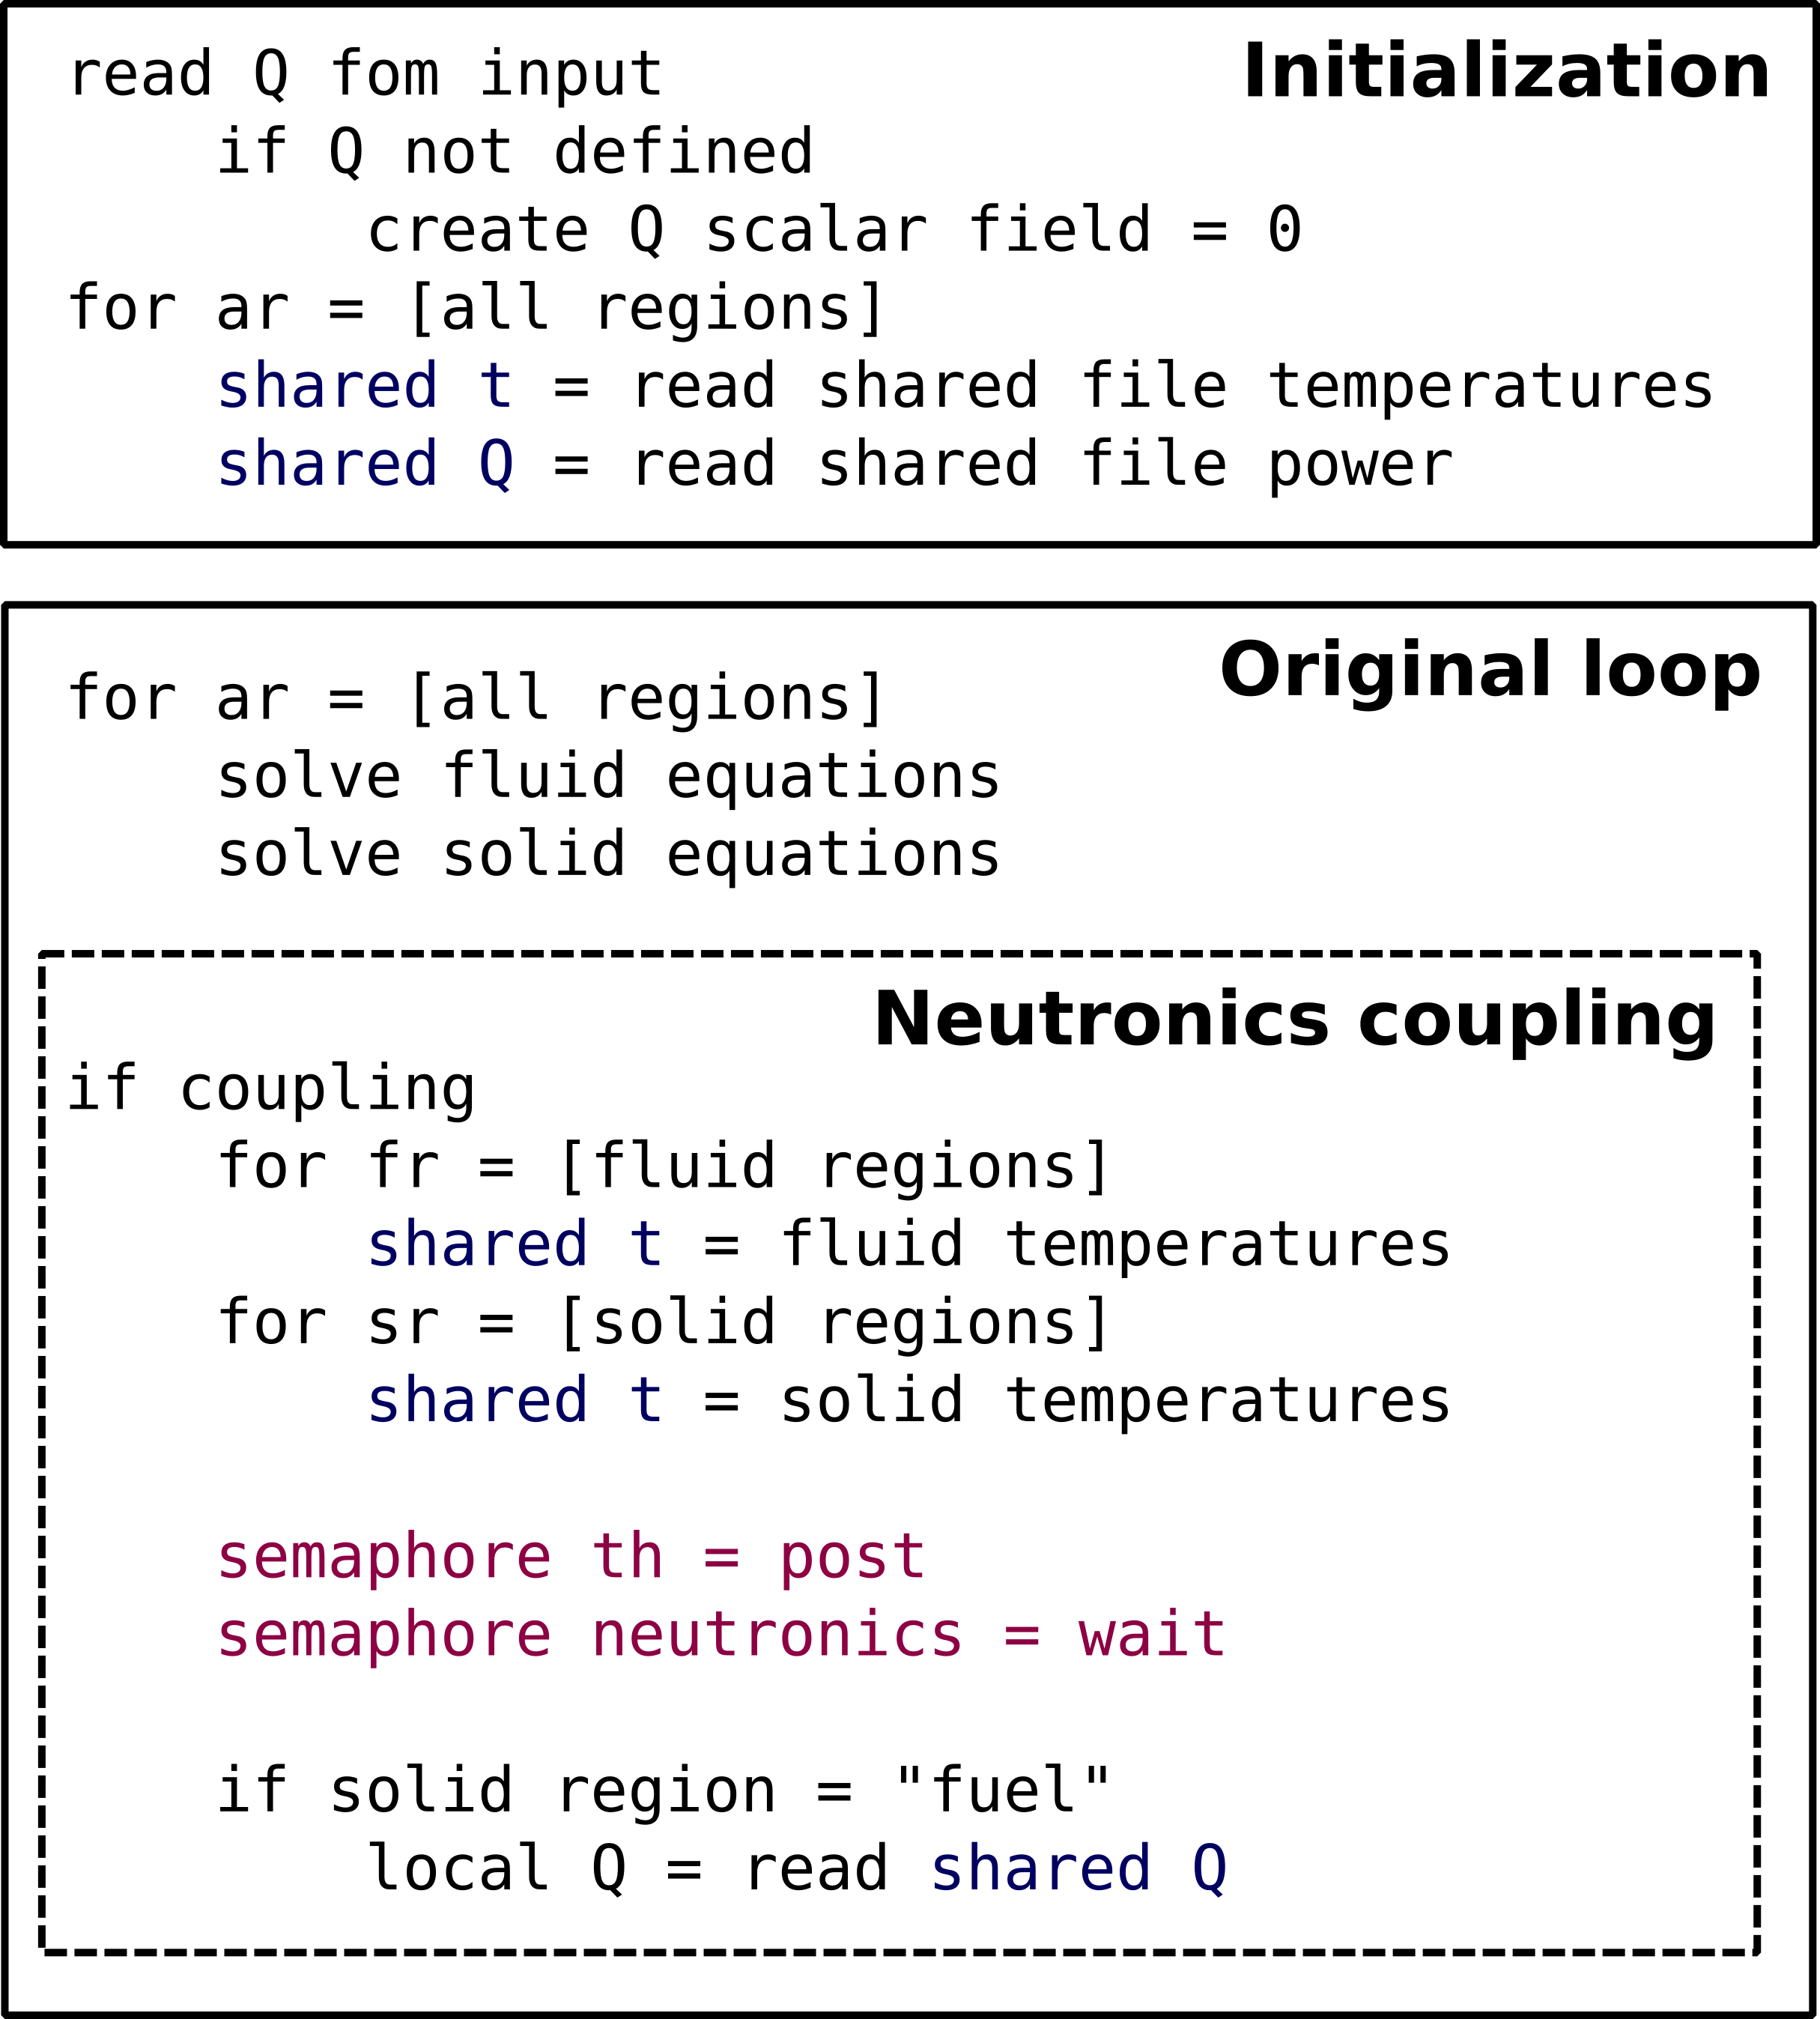
\includegraphics[scale=0.5]{figuras/algoritmo_openfoam.png}
  \label{fig:algo_th}
%  \legend{Fonte: autor}
\end{figure}

\begin{itemize}
\item \textbf{Inicialização:} Na inicialização do \textit{OpenFOAM}, é lido o valor inicial da potência para
  a simulação caso o arquivo de definição de potência esteja disponível. Caso contrário, a potência é inicializado
  com zero. Os espaços em memória compartilhada são verificados. Caso não estejam corretamente alocados, o sistema
  assume que o sistema executará de forma não-acoplada. Cabe lembrar, como dito no início da seção \ref{sec:acoplamento},
  o \textit{milonga} é iniciado antes do \textit{OpenFOAM} e, conforme será descrito no algoritmo da neutrônica, é
  ele o encarregado da alocação da memória compartilhada.

\item \textbf{Laço original:} Este é o laço do \textit{solver} original na sua execução do algoritmo SIMPLE. Este
  trecho não foi alterado em relação ao original e nesta etapa são resolvidas as respectivas equações
  para as regiões fluidas e sólidas. Ao fim
  deste laço, os valores de temperatura de cada célula de cada região estão calculados e disponíveis.

\item \textbf{Acoplamento com a neutrônica:} Caso seja o momento de troca de dados (a implementação atual
  executa uma chamada acoplada para cada 100 iterações da termo-hidráulica), para as regiões fluidas são copiados os valores
  de temperaturas para a memória compartilhada nas posições relativas às células das regiões fluidas. Em seguida, o mesmo
  é feito para as regiões sólidas. Com os valores calculados disponíveis na memória compartilhada, o \textit{OpenFOAM}
  avisa (post) no semáforo relativo à termo-hidráulica (th) que a memória compartilhada está liberada para uso. No próximo
  passo o \textit{OpenFOAM} lê o semáforo da neutrônica que, neste instante, indica que o \textit{OpenFOAM} aguarde. Quando
  receber o aviso (post) de liberação, o \textit{OpenFOAM} continua e, apenas para a região nomeada como combustível (fuel),
  lê os dados de potência disponíveis na memória compartilhada para sua estrutura de dados local, um campo escalar volumétrico
  de potências.
\end{itemize}

Ao fim da execução da etapa relativa ao acoplamento, o controle de execução volta ao laço original. A inicialização é
feita uma única vez para todos os passos de simulação.

\subsection{Algoritmo neutrônica}

\begin{figure}[htb]
  \caption{Algoritmo neutrônica.}
  \centering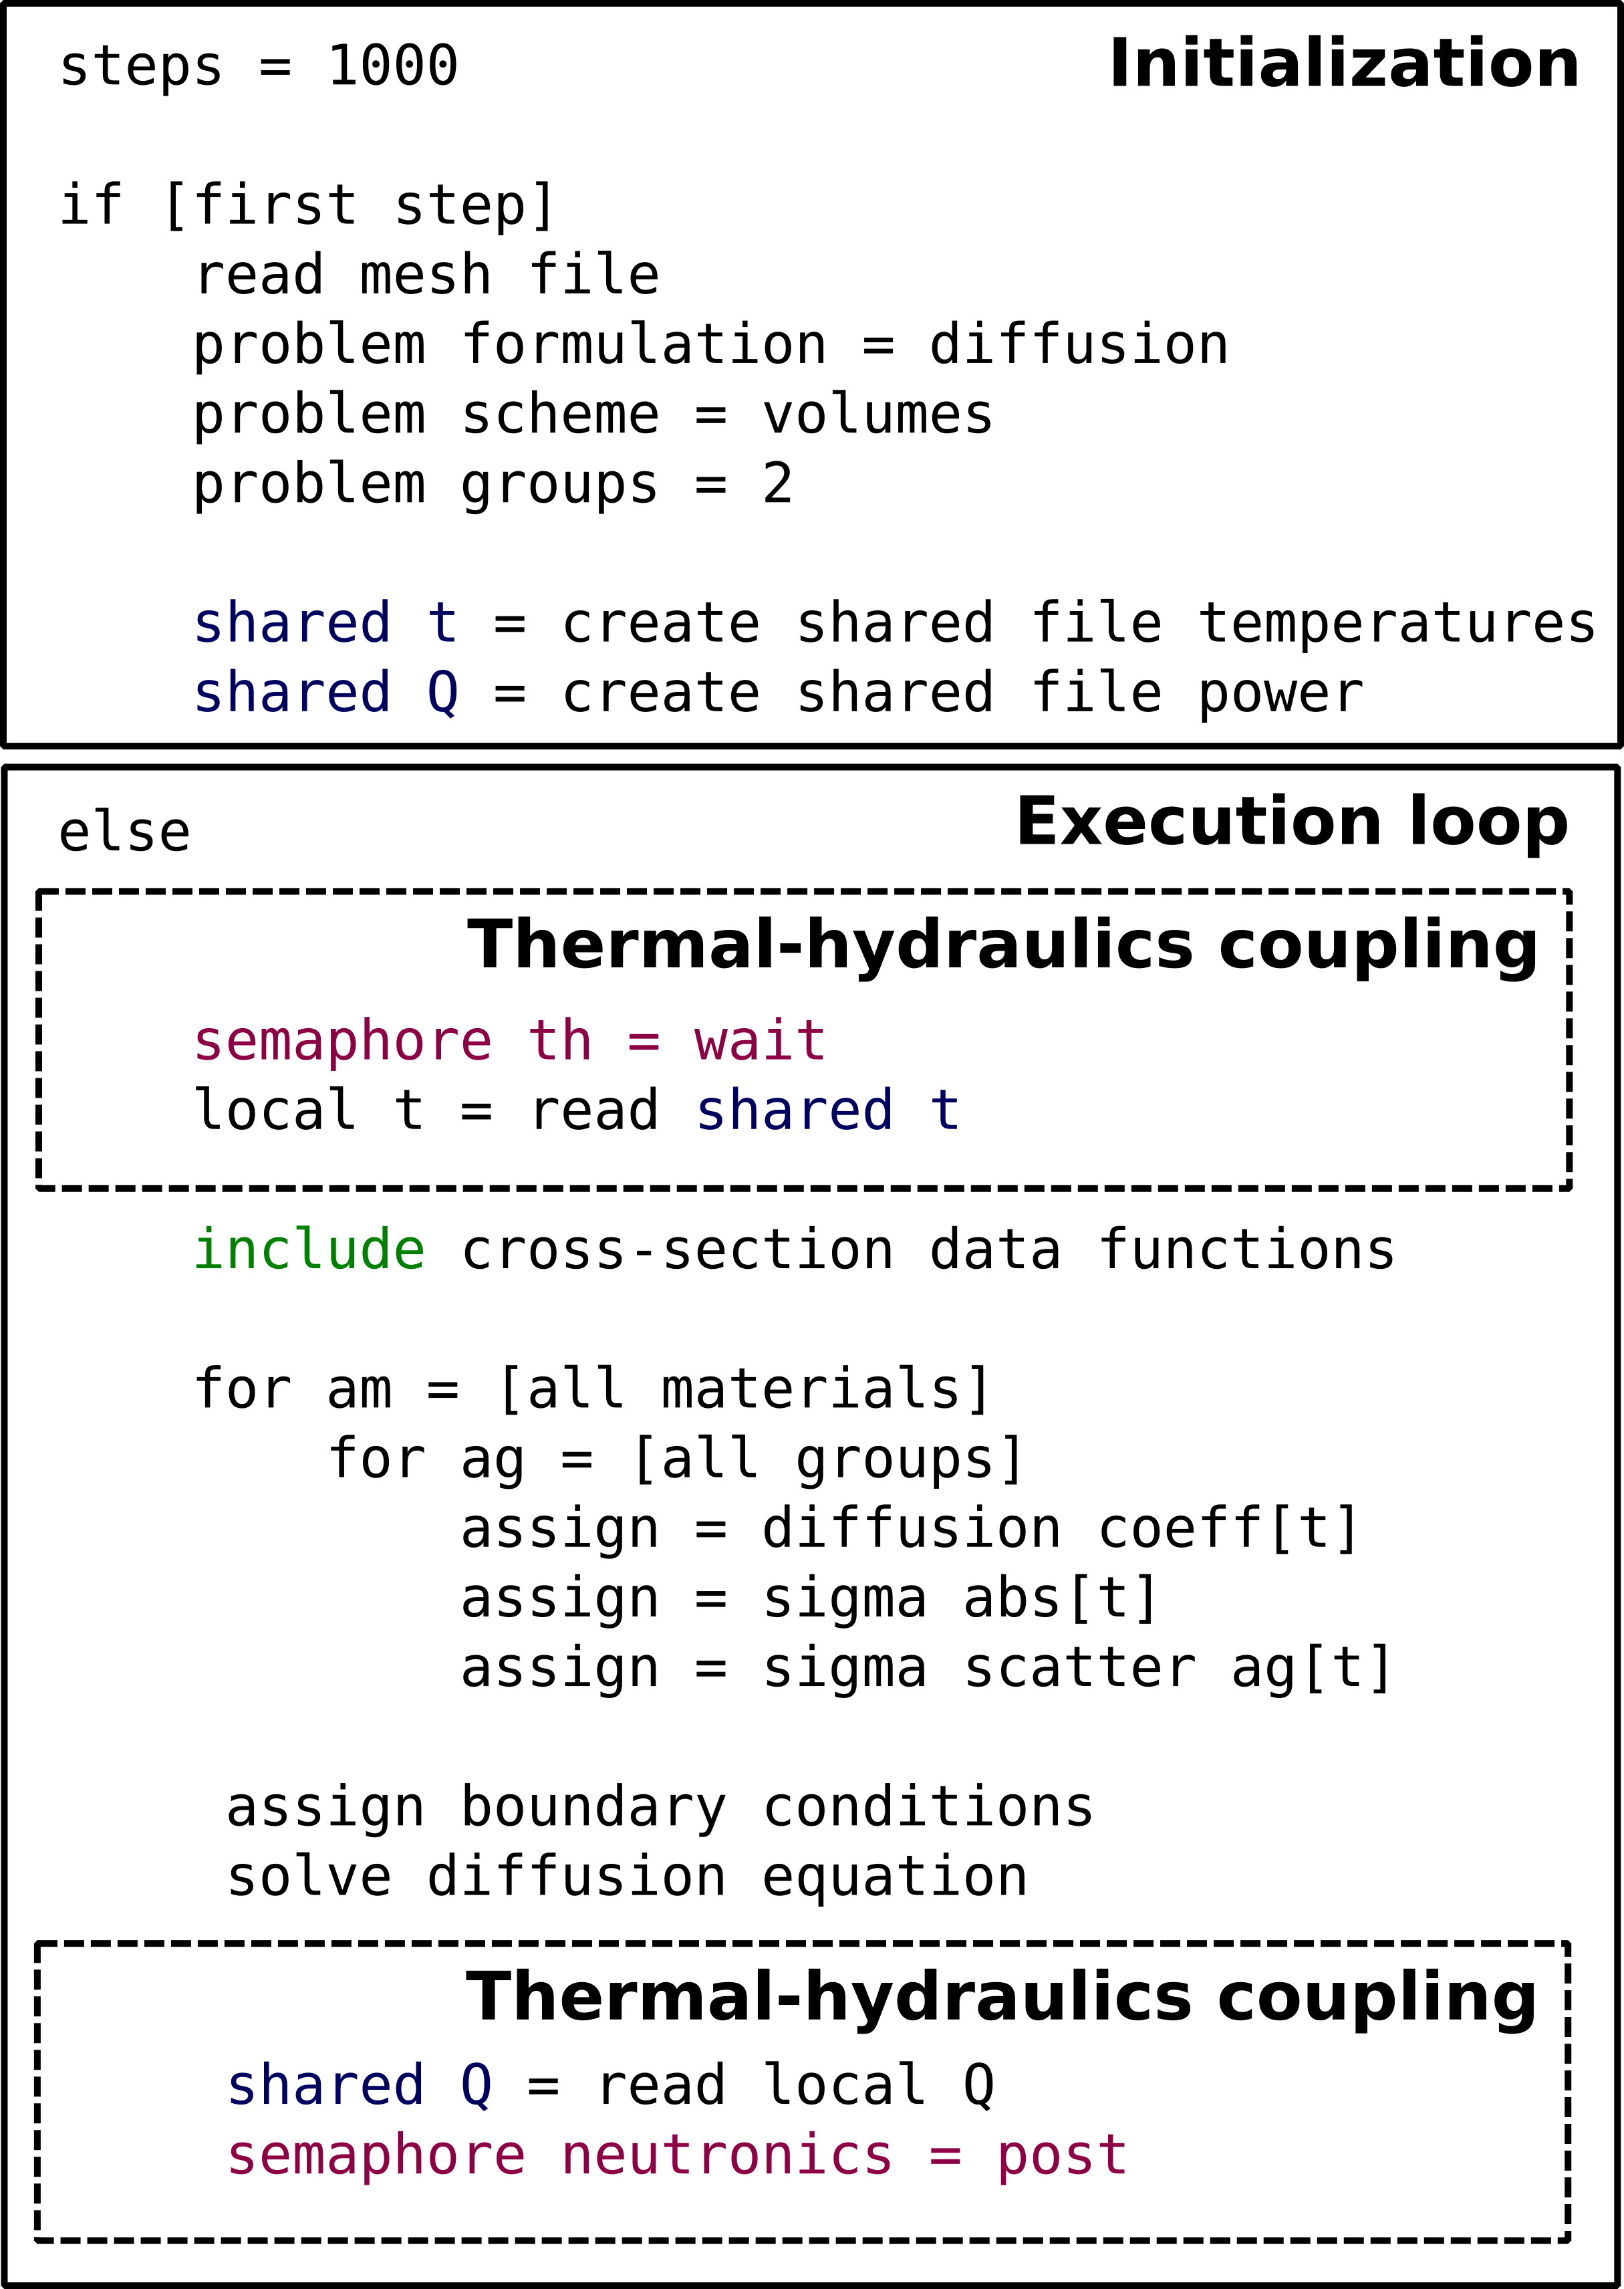
\includegraphics[scale=0.5]{figuras/algoritmos_milonga.png}
  \label{fig:algo_neutronica}
%  \legend{Fonte: autor}
\end{figure}





% -------------------------------------------------------------------------------------------------------
\subsection{Implementação: uma olhada no código-fonte.}
\label{subsec:detth}
Na seção \ref{sec:th} foram apresentadas as bases teóricas do problema termo-hidráulico.
Nesta sub-seção, são
descritas as alterações diversas promovidas no \textit{solver} original do \textit{OpenFOAM}
que foi chamado \texttt{thesisCoupledFoam}.

A principal alteração feita no \textit{solver} originalmente implementado foi a adição de um termo-fonte.
Esta alteração permite a geração de calor no sólido, útil tanto no problema acoplado
quanto numa eventual simulação isolada em que se deseje geração de
calor\footnote{A partir da versão 2.2, o \textit{OpenFOAM} introduziu em alguns dos seus
\textit{solvers}, incluindo o \texttt{chtMultiRegionSimpleFoam} a possibilidade de definição
de termo-fonte via \texttt{fvOptions}. Isso permite alteração da física do problema em
tempo de execução. Infelizmente, a forma de implementação desta funcionalidade não atendia uma
utilização do \textit{solver} de forma acoplada.}. Isso foi feito acrescentando-se uma estrutura
do tipo campo escalar volumétrico, estrutura de dados utilizada pelo \textit{OpenFOAM},
para armazenar os valores de potência a serem usados. Sendo assim, na sua inicialização,
o \textit{solver} modificado busca, além dos arquivos padrão para as grandezas calculadas, um
arquivo chamado \texttt{Q} que deve conter o campo volumétrico de potências em $W/m^3$. Caso
este arquivo não seja encontrado, é inicializado com valores nulos para o termo-fonte.

O trecho de código em que a leitura do campo volumétrico para a potência é feita
é apresentado na listagem \ref{lst:Q}.

\begin{lstlisting}[caption={Leitura/criação do campo volumétrico de potências.}\label{lst:Q}]
  PtrList<volScalarField> qVol(solidRegions.size());

  // Read Q if it exists. If not, create a null (zero) volScalarField
  IOobject Qfile("Q", runTime.timeName(), solidRegions[i],
                 IOobject::READ_IF_PRESENT, IOobject::AUTO_WRITE);

  // Must check it before creating the field
  if(Qfile.headerOk())
  {
    // Create a qvol field from dictionary
    qVol.set(i, new volScalarField (Qfile, solidRegions[i]));
  }
  else
  {
    // If file is not there, create a new IOobject
    // setting the dimensions of the field
    qVol.set(i,
    new volScalarField(IOobject
                          ("Q", runTime.path(), solidRegions[i], IOobject::NO_READ,
                              IOobject::AUTO_WRITE), solidRegions[i], dimensionedScalar
                          ("2", dimensionSet(1, -1, -3, 0, 0), scalar(0.0))
                          )
                      );
  }
\end{lstlisting}

Na linha $1$, é criada uma lista de ponteiros para campos escalares volumétricos. Essa estrutura
retém as referências para os campos volumétricos de potencias de todas as regiões sólidas. Na
presente implementação, apenas a região com nome \textbf{``fuel''} pode ter um valor não nulo
para o campo de potências. Na linha $4$ cria-se um objeto de entrada e saída de acordo com o
arquivo \textbf{``Q''}. Se o
objeto criado tiver o cabeçalho correto (linha $8$) é criada uma entrada na lista de referências com os
dados do arquivo (linha $11$). Caso contrário, se um arquivo mal-formado for encontrado ou
não for encontrado o arquivo, é criado um campo volumétrico escalar com valores nulos nas dimensões
esperadas (linhas $17$ a $23$). A partir deste ponto, o campo escalar volumétrico \textbf{``Q''}
está disponível para ser usado.

A criação do campo escalar volumétrico de potências é feito na inicialização dos campos dos materiais
sólidos, anterior ao algoritmo de solução. O algoritmo de solução usado é o SIMPLE
\textit{(Semi-Implicit Method for Pressur-Linked Equations}). Este algoritmo funciona
estimando um valor inicial para o cálculo da pressão e então fazendo correções no valor
estimado \cite{Versteeg2007}. Esse procedimento é repetido até que se chegue a um valor
aceitável dentro das condições de parada. Lembrando que este procedimento é feito para
a solução do escoamento. O \textit{solver} resolve separadamente cada região de acordo com seu
tipo, fluida ou sólida, tudo isso dentro da iteração do algoritmo SIMPLE.

Um fragmento do laço de iterações do algortimo SIMPLE é apresentado na listagem \ref{lst:simple}.

\begin{lstlisting}[caption={Fragmento do laço do algoritmo SIMPLE.}\label{lst:simple}]
  while (runTime.loop())
  {
    nIterations++;

    forAll(fluidRegions, i)
    {
      // Fluid regions loop: removed for the sake of clarity
    }
    
    forAll(solidRegions, i)
    {
      #include "setRegionSolidFields.H"
      #include "readSolidMultiRegionSIMPLEControls.H"
      #include "solveSolid.H"
      
      runTime.write();
    }
\end{lstlisting}

O controle da simulação é feito pelo objeto \texttt{runTime}, responsável por avaliar resíduos
e outras condições de parada. As regiões definidas como fluidas são resolvidas num laço (linha $5$)
e então são resolvidas as equações para as regiões sólidas (linha $10$). O \textit{OpenFOAM} utiliza-se
de uma diretiva de inclusão (linhas $12$ a $14$) para adicionar ao código-fonte o conteúdo de outros
arquivos definidos pelos nomes. Isso é feito com o objetivo de deixar o código-fonte mais legível como
também de evitar re-escrita de código, já que muitos dos arquivos incluídos são comuns a outros
\textit{solvers}. Um desses arquivos (linha $14$) é o que contém as equações a serem resolvidas para
a região sólida. É nele que o campos escalar volumétrico \textbf{``Q''} é utilizado. Um fragmento
do arquivo de solução de sólidos é apresentado na listagem \ref{lst:solvesolid}.

\begin{lstlisting}[caption={Fragmento do laço do algoritmo SIMPLE.}\label{lst:solvesolid}]
  {
    for (int nonOrth=0; nonOrth<=nNonOrthCorr; nonOrth++)
    {
      fvScalarMatrix hEqn
      (
      - fvm::laplacian(betav*alpha, h, "laplacian(alpha,h)")

      // Source-term added to que equation
      - Q
      );

      hEqn.relax();
      hEqn.solve();
    }
  }
\end{lstlisting}

Dentro de um laço interno para correção de não-ortogonalidade, é definida a matriz de solução
referente a entalpia (linha $4$). Como argumentos do objeto matriz sendo criado, é adicionado
o termo-fonte \textbf{``Q''} (linha $9$). Estas são as principais
modificações no código-fonte do \textit{solver} para
acrescentar o termo-fonte à equação do calor no sólido.

Outra modificação importante é a adição de estruturas de dados capazes de fazer a comunicação
por memória compartilhada.
***

ESCREVER

***

% ------------------------------------------------------------------------------------------------

% codigo e explicação de shared memory.

% -------------------------------------------------------------------------------------------------
Espera-se, ao apresentar algumas das implementações feitas em fragmentos do código-fonte
do \textit{OpenFOAM}, familiarizar o leitor com o formato interno do \textit{OpenFOAM}
e alguns detalhes de como se deu, na prática, a parte da metodologia de acoplamento
desenvolvida nesta tese em relação às alterações no código-fonte do \textit{OpenFOAM}.

Ao leitor interessado em aprofundar-se nos detalhes técnicos da implementação, fica o
convite a examinar livremente código-fonte do \textit{solver} \texttt{thesisCoupleFoam}, disponível
no repositório \texttt{https://github.com/vitorvas/thesisChtMultiRegionFoam}.




































%Modelada uma geometria idêntica à representada na malha utilizada pelo \textit{OpenFOAM},
%foram feitas simulações da neutrônica pelo Serpent com objetivo de obter as seções
%de choque em dois grupos a serem usadas na solução da aproximação por difusão dos nêutrons
%pelo \textit{milonga}.

%Na saída do Serpent são dados constantes de groups homogeneizadas (neste caso, com espectro
%corrigido para fugas pelo método B1 \textbf{CITAR}) e outros parâmetros de interesse para
%a modelagem por difusão como, por exemplo, os coeficientes de difusão para cada grupo já
%calculados.

%Como todos os elementos do desenvolvimento estão relacionados entre si, sempre que
%julgado oportuno para a clareza do entendimento, os conceitos desenvolvidos em cada
%seção poderão ser apresentados conjuntamente. De fato, uma vez que o problema multifísica
%(ou acoplamento) nada mais é do que a solução conjunta de dois problemas que são,
%usualmente, resolvidos separadamente, é natural como definir, modelar e resolver os
%dois problemas separadamente.

%De acordo com as definições de problemas acoplados apresentadas
%no capítulo \ref{chap:rev}, ao resolver os problemas neutrônico e termo-hidráulico
%separadamente, o acoplamento ainda pode ser considerado implícito de acordo com, já que a troca de informações entre os problemas ocorre ao nível de termos completos,
%e não em condições de contorno. É importante dizer que essa nomeclatura para as formas
%de acoplamento não é unânime na literatura \cite{Ivanov2007}.

%Deve estar claro que a metodologia a ser descrita trata do ciclo de desenvolvimento
%do \textit{software} acoplado. Apesar de ser possível considerar as simulações e
%os processos de pré-processamento e pós-processamento, tanto termo-hidráulicos quanto
%neutrônicos, optou-se por tratar destas etapas exclusivamente na seção de validação e,
%quando pertinente, nos resultados obtidos.


%Na figura \ref{metodoetapas} são apresentadas as relações entre os diferentes elementos
%do sistema acoplado.







% ----------------------------------------------------------
% Aplicação
% ----------------------------------------------------------
% ----------------------------------------------------------
% Aplicação
% ----------------------------------------------------------
\chapter{Aplicação}
\label{chap:aplicacao}


\section{Modelo}

%\begin{figure}[htb]
%  \caption{Aplicação: o sistema acoplado.}
%  \centering\includegraphics[scale=0.7]{figuras/aplicacao1.png}
%  \label{metodoetapas}
%  \legend{Fonte: autor}
%\end{figure}

\section{Geração de seções de choque}

Descrever o trabalho da Patrícia citando \cite{Reis2015}.

% Quatro tabelas para as quatro temperaturas
% Usa o package {multirow}

% Tabela para os valores
\begin{tabular}{ l | c | r}
  \hline
  \multicolumn{3}{ c }{Coeficientes Mnemônicos} \\
  \hline
  \multirow{4}{*}{Grupo 1: > 0,625 MeV} & Diffusion coefficient & $D1$\\
& Absorption cross-section & $\Sigma A1$\\
& Scattering cross-section & $\Sigma S1.2$\\
  & Neutrons per fission * Fission cross-section & $\nu \Sigma F1$\\
  \hline
\multirow{3}{*}{Grupo 2: < 0,625 MeV} & Diffusion coefficient & $D2$\\
& Absorption cross-section & $\Sigma A2$\\
& Neutrons per fission * Fission cross-section & $\nu \Sigma F2$ \\
\hline
\end{tabular}


\begin{tabular}{r l l l l}
  \multicolumn{5}{c}{Fuel} \\
  \hline
  Parâmetro & $300K$ & $400K$ & $500K$ & $600K$ \\
  \hline
  $D1$ & & & & \\
  $\Sigma A1$ & & & & \\
  $\Sigma S1.2$ & & & & \\
  $\nu \Sigma F1$ & & & & \\
  \hline
  $D2$ & & & & \\
  $\Sigma A2$ & & & & \\
  $\nu \Sigma F2$ & & & & \\
  \hline
\end{tabular}

\begin{tabular}{r l l l l}
  \multicolumn{5}{c}{Cladding} \\
  \hline
  Parâmetro & $300K$ & $400K$ & $500K$ & $600K$ \\
  \hline
  $D1$ & & & & \\
  $\Sigma A1$ & & & & \\
  $\Sigma S1.2$ & & & & \\
  $\nu \Sigma F1$ & & & & \\
  \hline
  $D2$ & & & & \\
  $\Sigma A2$ & & & & \\
  $\nu \Sigma F2$ & & & & \\
  \hline
\end{tabular}

\begin{tabular}{r l l l l}
  \multicolumn{5}{c}{Coolant} \\
  \hline
  Parâmetro & $300K$ & $400K$ & $500K$ & $600K$ \\
  \hline
  $D1$ & & & & \\
  $\Sigma A1$ & & & & \\
  $\Sigma S1.2$ & & & & \\
  $\nu \Sigma F1$ & & & & \\
  \hline
  $D2$ & & & & \\
  $\Sigma A2$ & & & & \\
  $\nu \Sigma F2$ & & & & \\
  \hline
\end{tabular}


% ----------------------------------------------------------
% Resultados
% ----------------------------------------------------------
% ----------------------------------------------------------
% Resultados
% ----------------------------------------------------------
\chapter{Resultados (ou Prova do Conceito)}
\label{chap:resultados}

%Temos nesta tese o desenvolvimento de um sistema de cálculos neutrônicos
%e termo-hidráulicos acoplados. Dentre as várias etapas de garantia de seu
%funcionamento, a primeira e imediata consiste e verificar\footnote{Existe
%  uma variedade de significados da palavra verificar em diferentes ramos
%  da Engenharia e na Computação. Nesta tese, verificar significa apenas
%  garantir que o sistema proposto faz o que foi projetado para fazer.} se
%os os dados são corretamente trocados entre os sitemas acoplados, se
%os cálculos em ambos convergem numericamente e se o modelo de teste
%se comporta da forma fisicamente esperada.

A utilização da expressão ``prova de conceito''\footnote{Do inglês ``proof of concept''. Definição do dicionário
  \textit{Oxford:[mass noun] Evidence, typically deriving from an experiment or pilot project, which demonstrates that a design concept,
    business proposal, etc. is feasible:‘In academia, he says, a narrowly focused solution is acceptable as a proof of concept.’}}
no título deste capítulo não é arbitraria.
Muito pelo contrário. ``prova de conceito'' significa a execução (ou implementação) de
certa ideia ou método de forma a demonstrar que tal ideia ou método funcionam. Melhor dizendo,
é a demonstração de um princípio com o objetivo de verificar seu potencial prático.

Sendo assim, de forma a testar a implementação desenvolvida, foram feitos dois conjuntos
separados de simulações, seguindo as modelagens físicas e numéricas apresentadas no Capítulo \ref{chap:aplicacao}
desta tese. De modo a capturar os efeitos da variação da temperatura dos distintos materiais
no fluxo neutrônico e, consequentemente, na potência gerada, foram feitas simulações
para três diferentes potências nominais. Estas simulações, foram feitas para dois casos
distintos: um sistema não-acoplado e para o sistema acoplado desenvolvido, totalizando seis
simulações. Na tabela
\ref{tab:setup} estão classificados os conjuntos de simulações realizados.

\begin{table}[htb]
  \centering
\caption[Casos e potências simuladas.]{Casos e potências simuladas}
\label{tab:setup}
\begin{tabular}{cccc}
Caso         & \multicolumn{3}{c}{\begin{tabular}[c]{@{}c@{}}Potências\\ (equivalente núcleo)\end{tabular}}                                                                                                                             \\ \hline
Não-acoplado & \begin{tabular}[c]{@{}c@{}}1.98 kW\\ (50 kW)\end{tabular}              & \begin{tabular}[c]{@{}c@{}}3.97 kW\\ (100 kW)\end{tabular} & \begin{tabular}[c]{@{}c@{}}7.93 kW\\ (200 kW)\end{tabular} \\ \hline
Acoplado     & \begin{tabular}[c]{@{}c@{}}1.98 kW\\  (50 kW)\end{tabular} & \begin{tabular}[c]{@{}c@{}}3.97 kW\\ (100 kW)\end{tabular} & \begin{tabular}[c]{@{}c@{}}7.93 kW\\ (200 kW)\end{tabular}
\end{tabular}
\end{table}
Cabe lembrar que para esta prova de conceito, foi utilizada apenas uma única malha para todos os casos.

% ------------------------------------------------------------------------------------------------------------
\section{Caso não-acoplado}
\label{sec:non-cp}

O conjunto de simulações realizadas para este caso foi feito de modo a ser referência para o outro conjunto
de simulações. Apesar de chamado ``não-acoplado'', pode ser considerado um caso ``inicialmente acoplado''.
Esta afirmação ficará mais clara observando a lista de etapas para a geração da condição inicial de potência
para o sistema:

\begin{enumerate}
\item Execução do \textit{OpenFOAM} com temperaturas iniciais homogêneas (temperatura ambiente) e distribuição nominal de potência homogênea;
\item Pós-processamento destas simulações para obtenção da temperatura média em cada material; %\ref{tab:temp-keff};
\item Obtenção das seções de choque para as temperaturas médias a partir da função de interpolação de temperaturas
  de referência (Tabela \ref{tab:temp} do Capítulo \ref{chap:aplicacao});
\item Execução do \textit{milonga} com as seções de choque correspondentes a cada temperatura média;
\item Pós-processamento destas simulações para adaptação das distribuições de potência obtidas pelo \textit{milonga}
  para condição inicial do problema no \textit{OpenFOAM};
\end{enumerate}

As temperaturas médias utilizadas e os fatores de multiplicação obtidos na geração da distribuição inicial
de potências são apresentados na tabela \ref{tab:temp-keff}.

\begin{table}[htb]
  \centering
\caption{Temperaturas e fator de multiplicação efetivo: cálculo não-acoplado.}
\label{tab:temp-keff}
\begin{tabular}{ccccc}
\multicolumn{1}{l}{}         & \multicolumn{3}{c}{Temperaturas [K]}                                                                      & \multicolumn{1}{l}{}     \\ \cline{2-4}
\multicolumn{1}{c}{Potência [kW]} & \multicolumn{1}{c}{Refrigerante} & \multicolumn{1}{c}{Revestimento} & \multicolumn{1}{c}{Combustível} & \multicolumn{1}{c}{$k_{eff}$} \\ \hline
1.98                      & 303,56                         & 327,20                         & 339,80                        & 1,15289                  \\ \hline
3.97                      & 307,15                         & 354,54                         & 379,77                        & 1,15117                  \\ \hline
7,93                      & 310,09                         & 375,42                         & 422,94                        & 1,14829                 
\end{tabular}
\end{table}

O caso não-acoplado nada mais é do que uma simulação termo-hidráulica utilizando como distribuição de potência
inicial o resultado obtido pelos cálculos neutrônicos com seções de choque constantes. Que por sua vez, foram
obtidas para temperaturas médias nos materiais calculadas pela termo-hidráulica com distribuição de potência
homogênea.

As distribuições de potências obtidas para os volumes de combustível podem ser vistas na Figura \ref{fig:pot-nc}.

\begin{figure}[htb]
  \caption[Distribuição de potência para os três casos simulados.]{Distribuição de potência para os três casos simulados.}
  \centering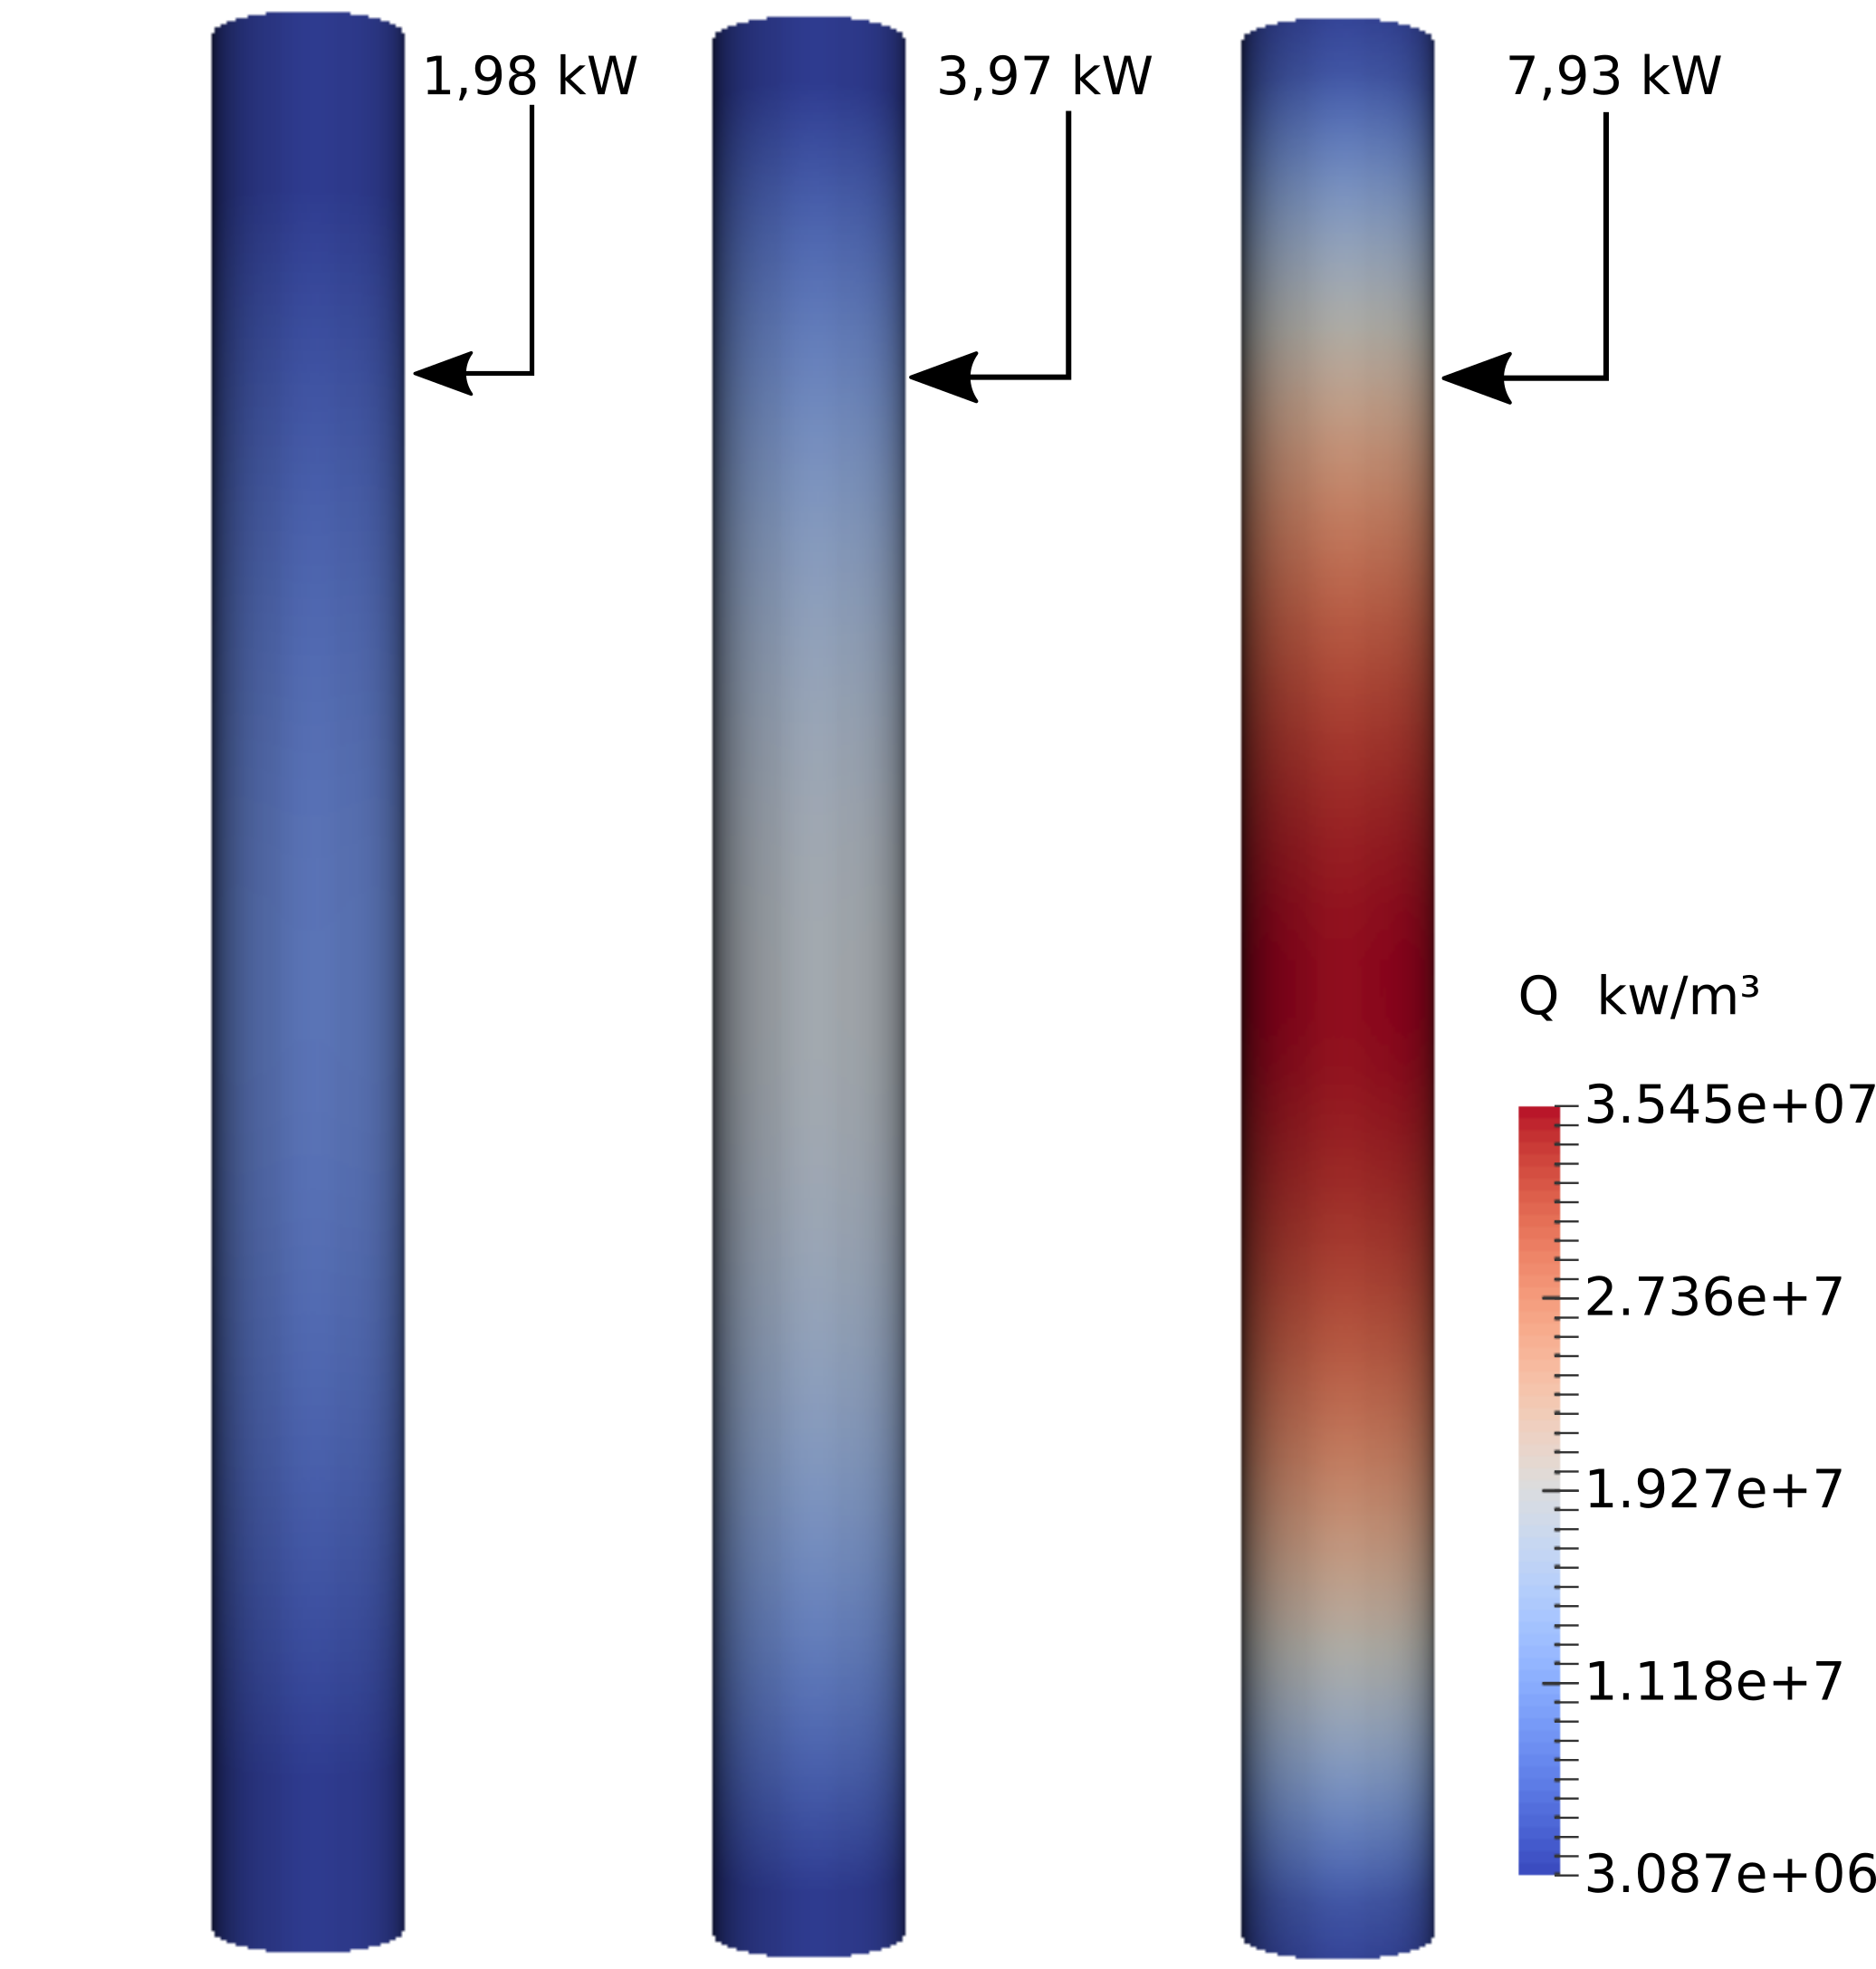
\includegraphics[scale=0.5]{figuras/Q_fuel_all_NC.png}
  \label{fig:pot-nc}
%  \legend{Fonte: autor}
\end{figure}

As distribuições de potência axial obedeceram, para os três casos, a perfis
cossenoidais, como pode ser visto na Figura \ref{fig:perf-nac-axial}. Estes são os perfis esperados para
os combustíveis modelados \cite{Veloso2005}. As distribuições de potência radiais -
obtidas do corte no ponto médio do modelo do combustível - possuem perfis diferentes, na Figura \ref{fig:perf-Q-nac-radial},
dos obtidos axialmente. A primeira e principal diferença está na abruta subida a partir da potência nula
no início e fim da curva. A razão para este comportamento é simples: apenas o combustível gera potência, sendo
zero para as regiões de revestimento e água (não apresentadas na curva). O achatamento na posição central
da curva em relação aos picos é devido ao menor fluxo térmico no centro do combustível. Nas regiões limite
entre o combustível e o revestimento, é maior o fluxo de nêutrons termalizados pela interação com o refrigerante (água).
Esse perfil é esperado em combustíveis do tipo TRIGA \cite{Ravnik1990}.

\begin{figure}[htb]
  \caption{Perfil de potência axial para os três casos simulados.}
  \centering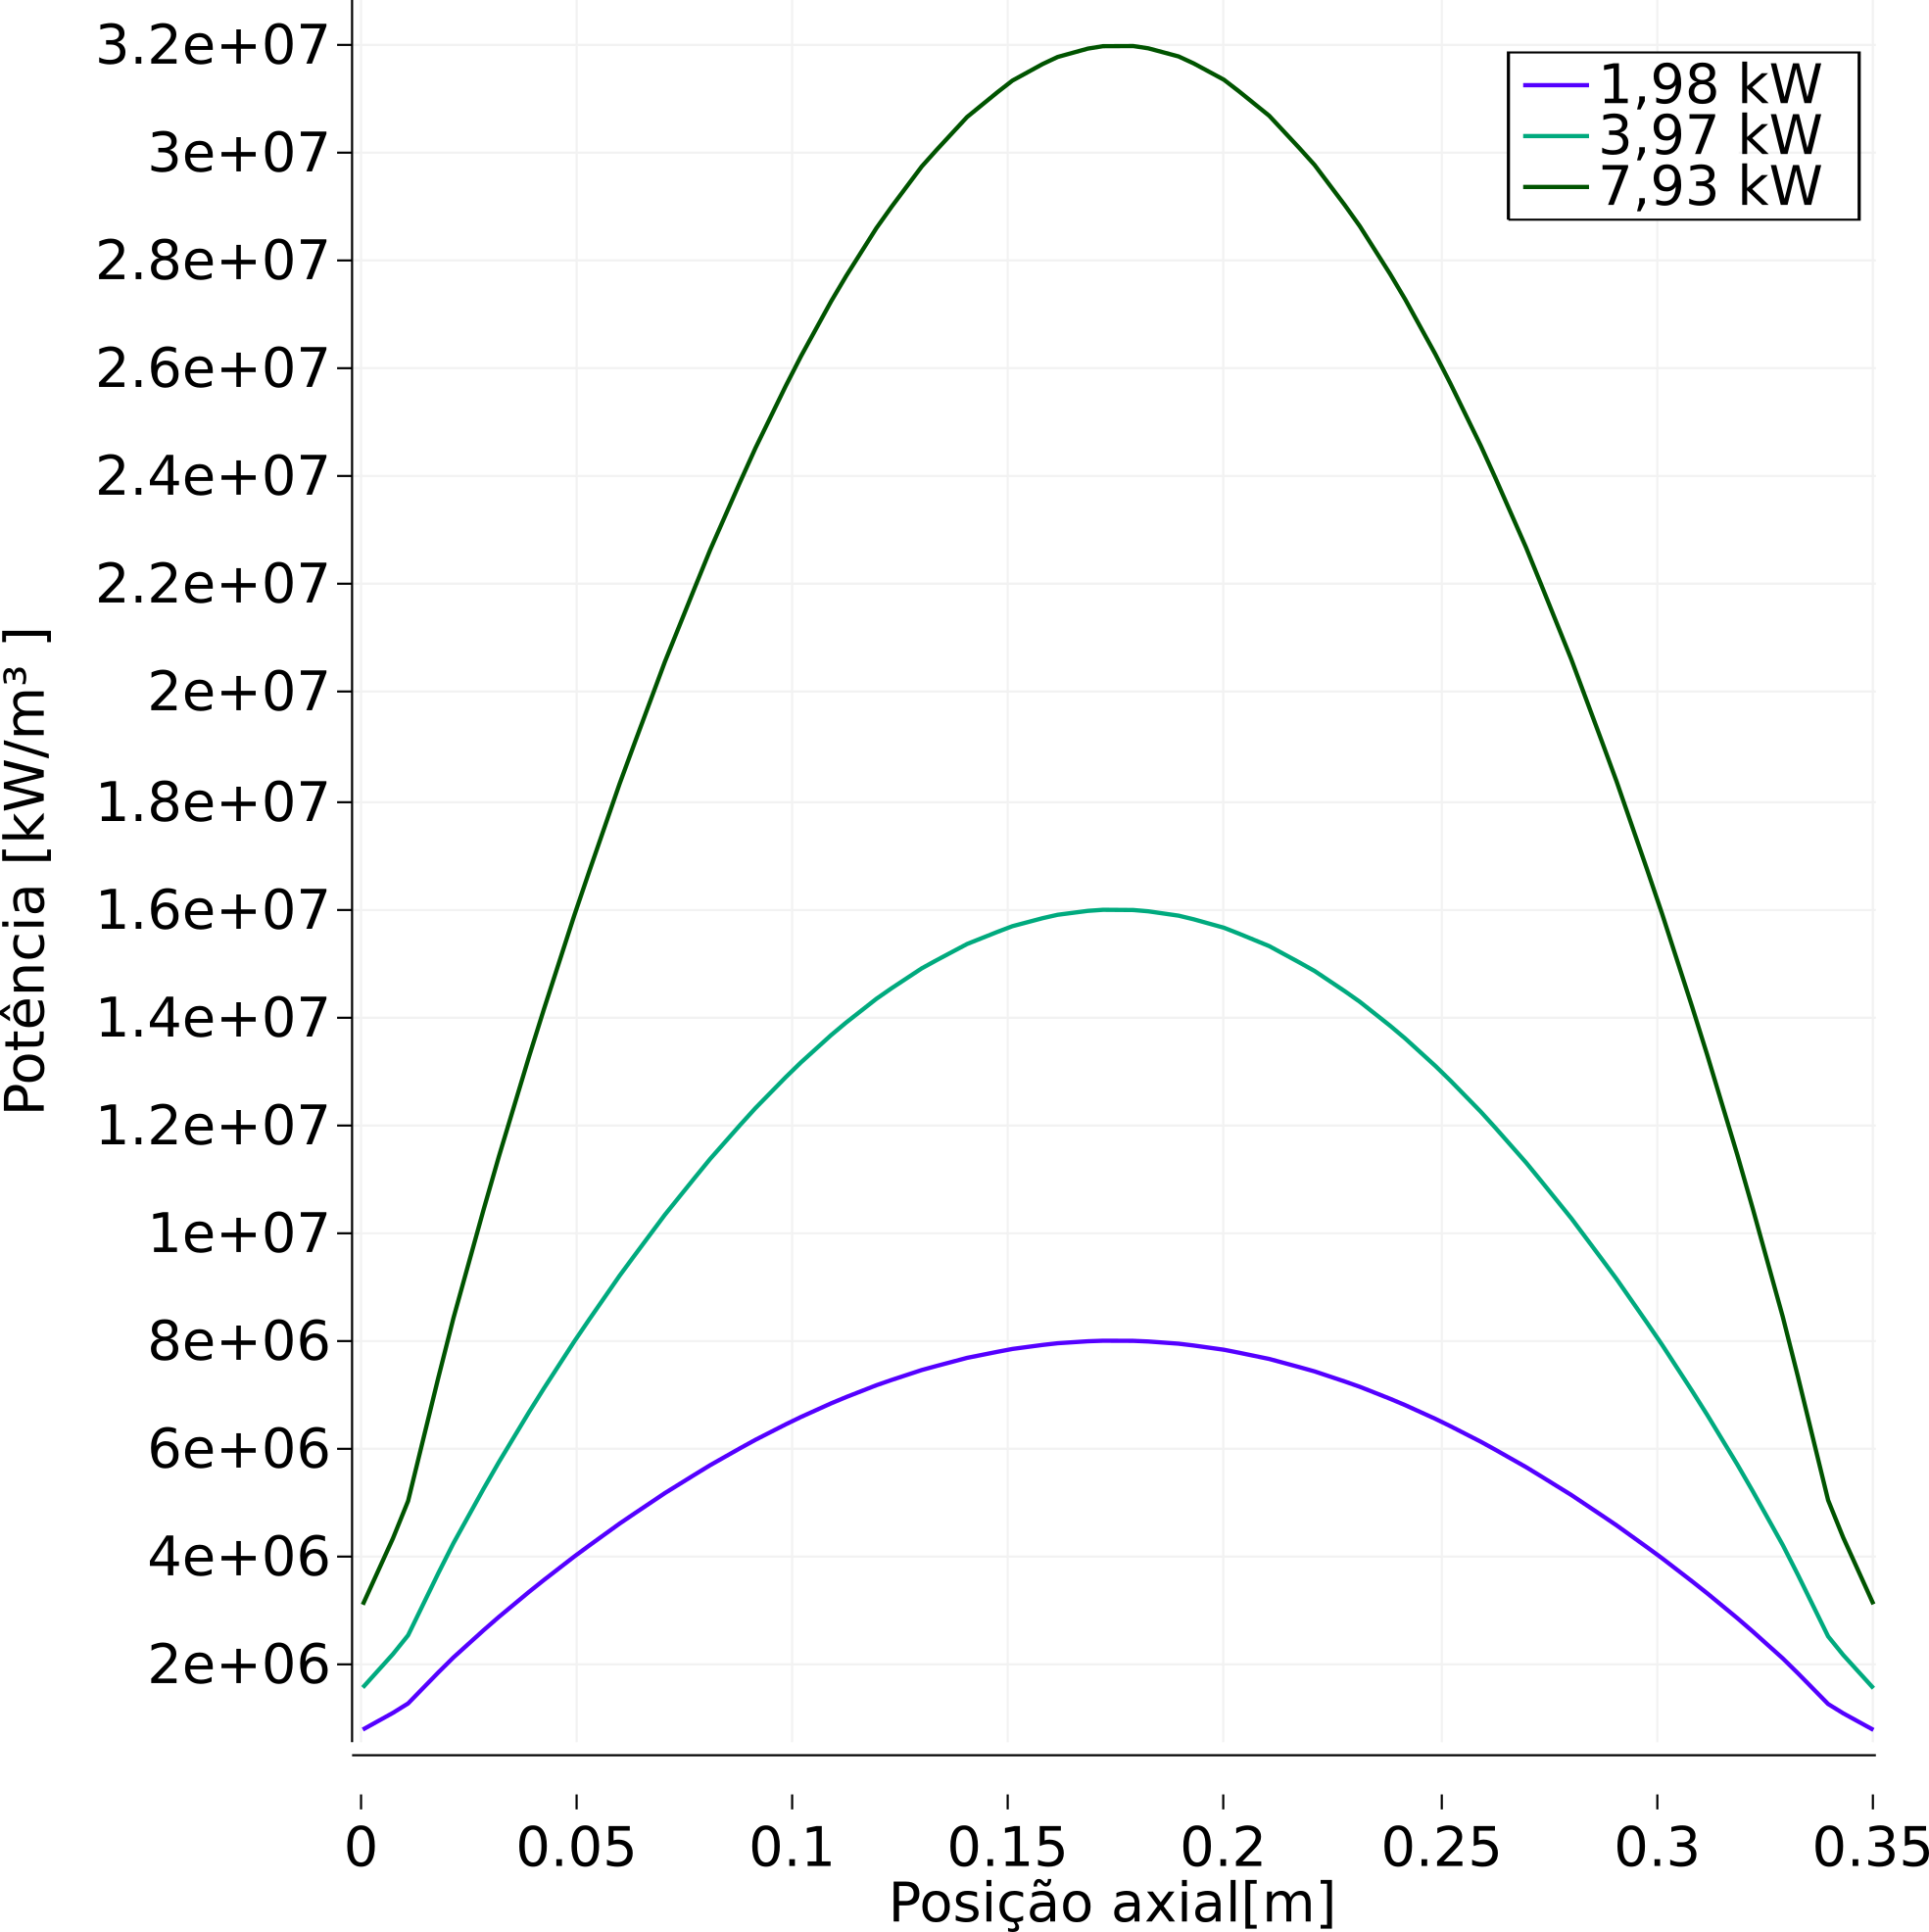
\includegraphics[scale=0.5]{figuras/Q_all_NC_port.png}
  \label{fig:perf-nac-axial}
%  \legend{Fonte: autor}
\end{figure}

\begin{figure}[htb]
  \caption[Perfil de potência radial para os três casos simulados.]{Perfil de potência radial para os três casos simulados.}
  \centering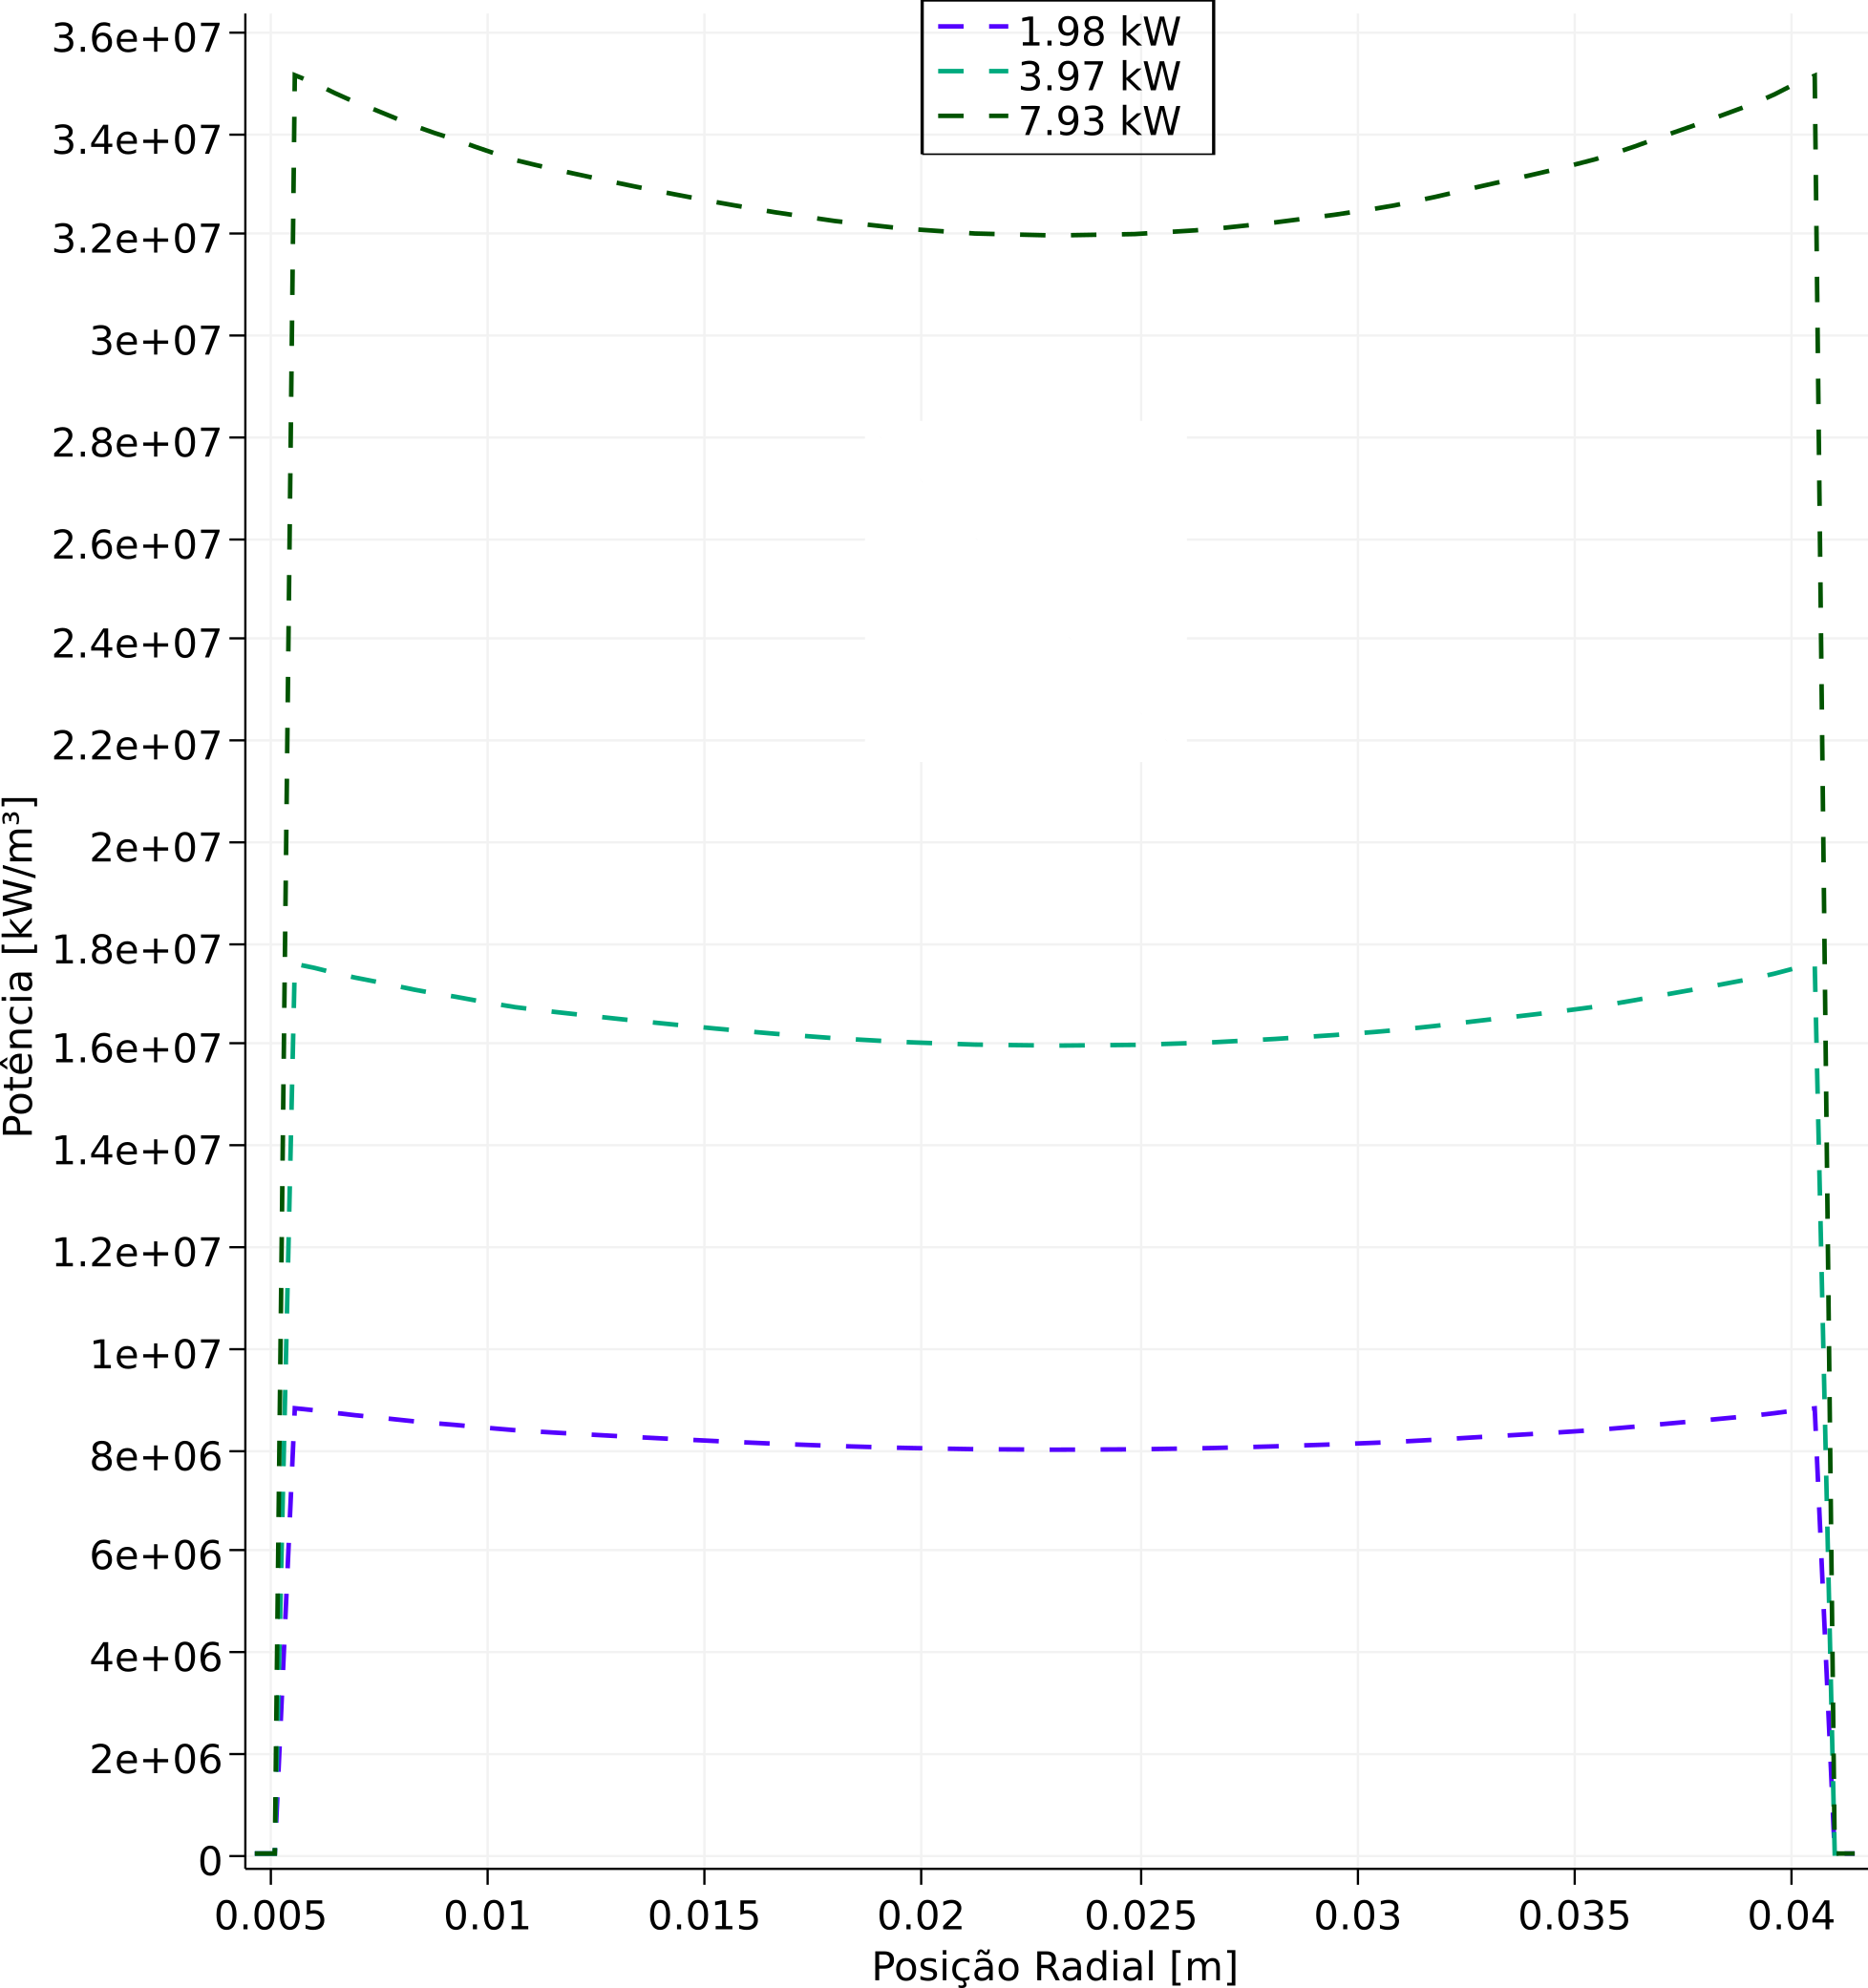
\includegraphics[scale=0.5]{figuras/Q_x_NC_square_port.png}
  \label{fig:perf-Q-nac-radial}
%  \legend{Fonte: autor}
\end{figure}

Os perfis de temperatura obtidos axialmente, Figura \ref{fig:perf-t-nac-axial},
apresentam, novamente para os três casos, uma diferença entre as extremidades
do combustível. Essa diferença é provocada pela escoamento do refrigerante (água) no
modelo. A água entra no sistema à temperatura constante de $300 K$ e, no seu trajeto,
absorve energia do sistema. Essa absorção é maior no na entrada (\textit{inlet}),
levando a uma maior resfriamento do sistema neste ponto do escoamento. Esse efeito
ocorre em todos os casos, apenas com diferença nas temperaturas de cada material.

\begin{figure}[htb]
  \caption{Perfil de temperaturas axial para os três casos simulados.}
  \centering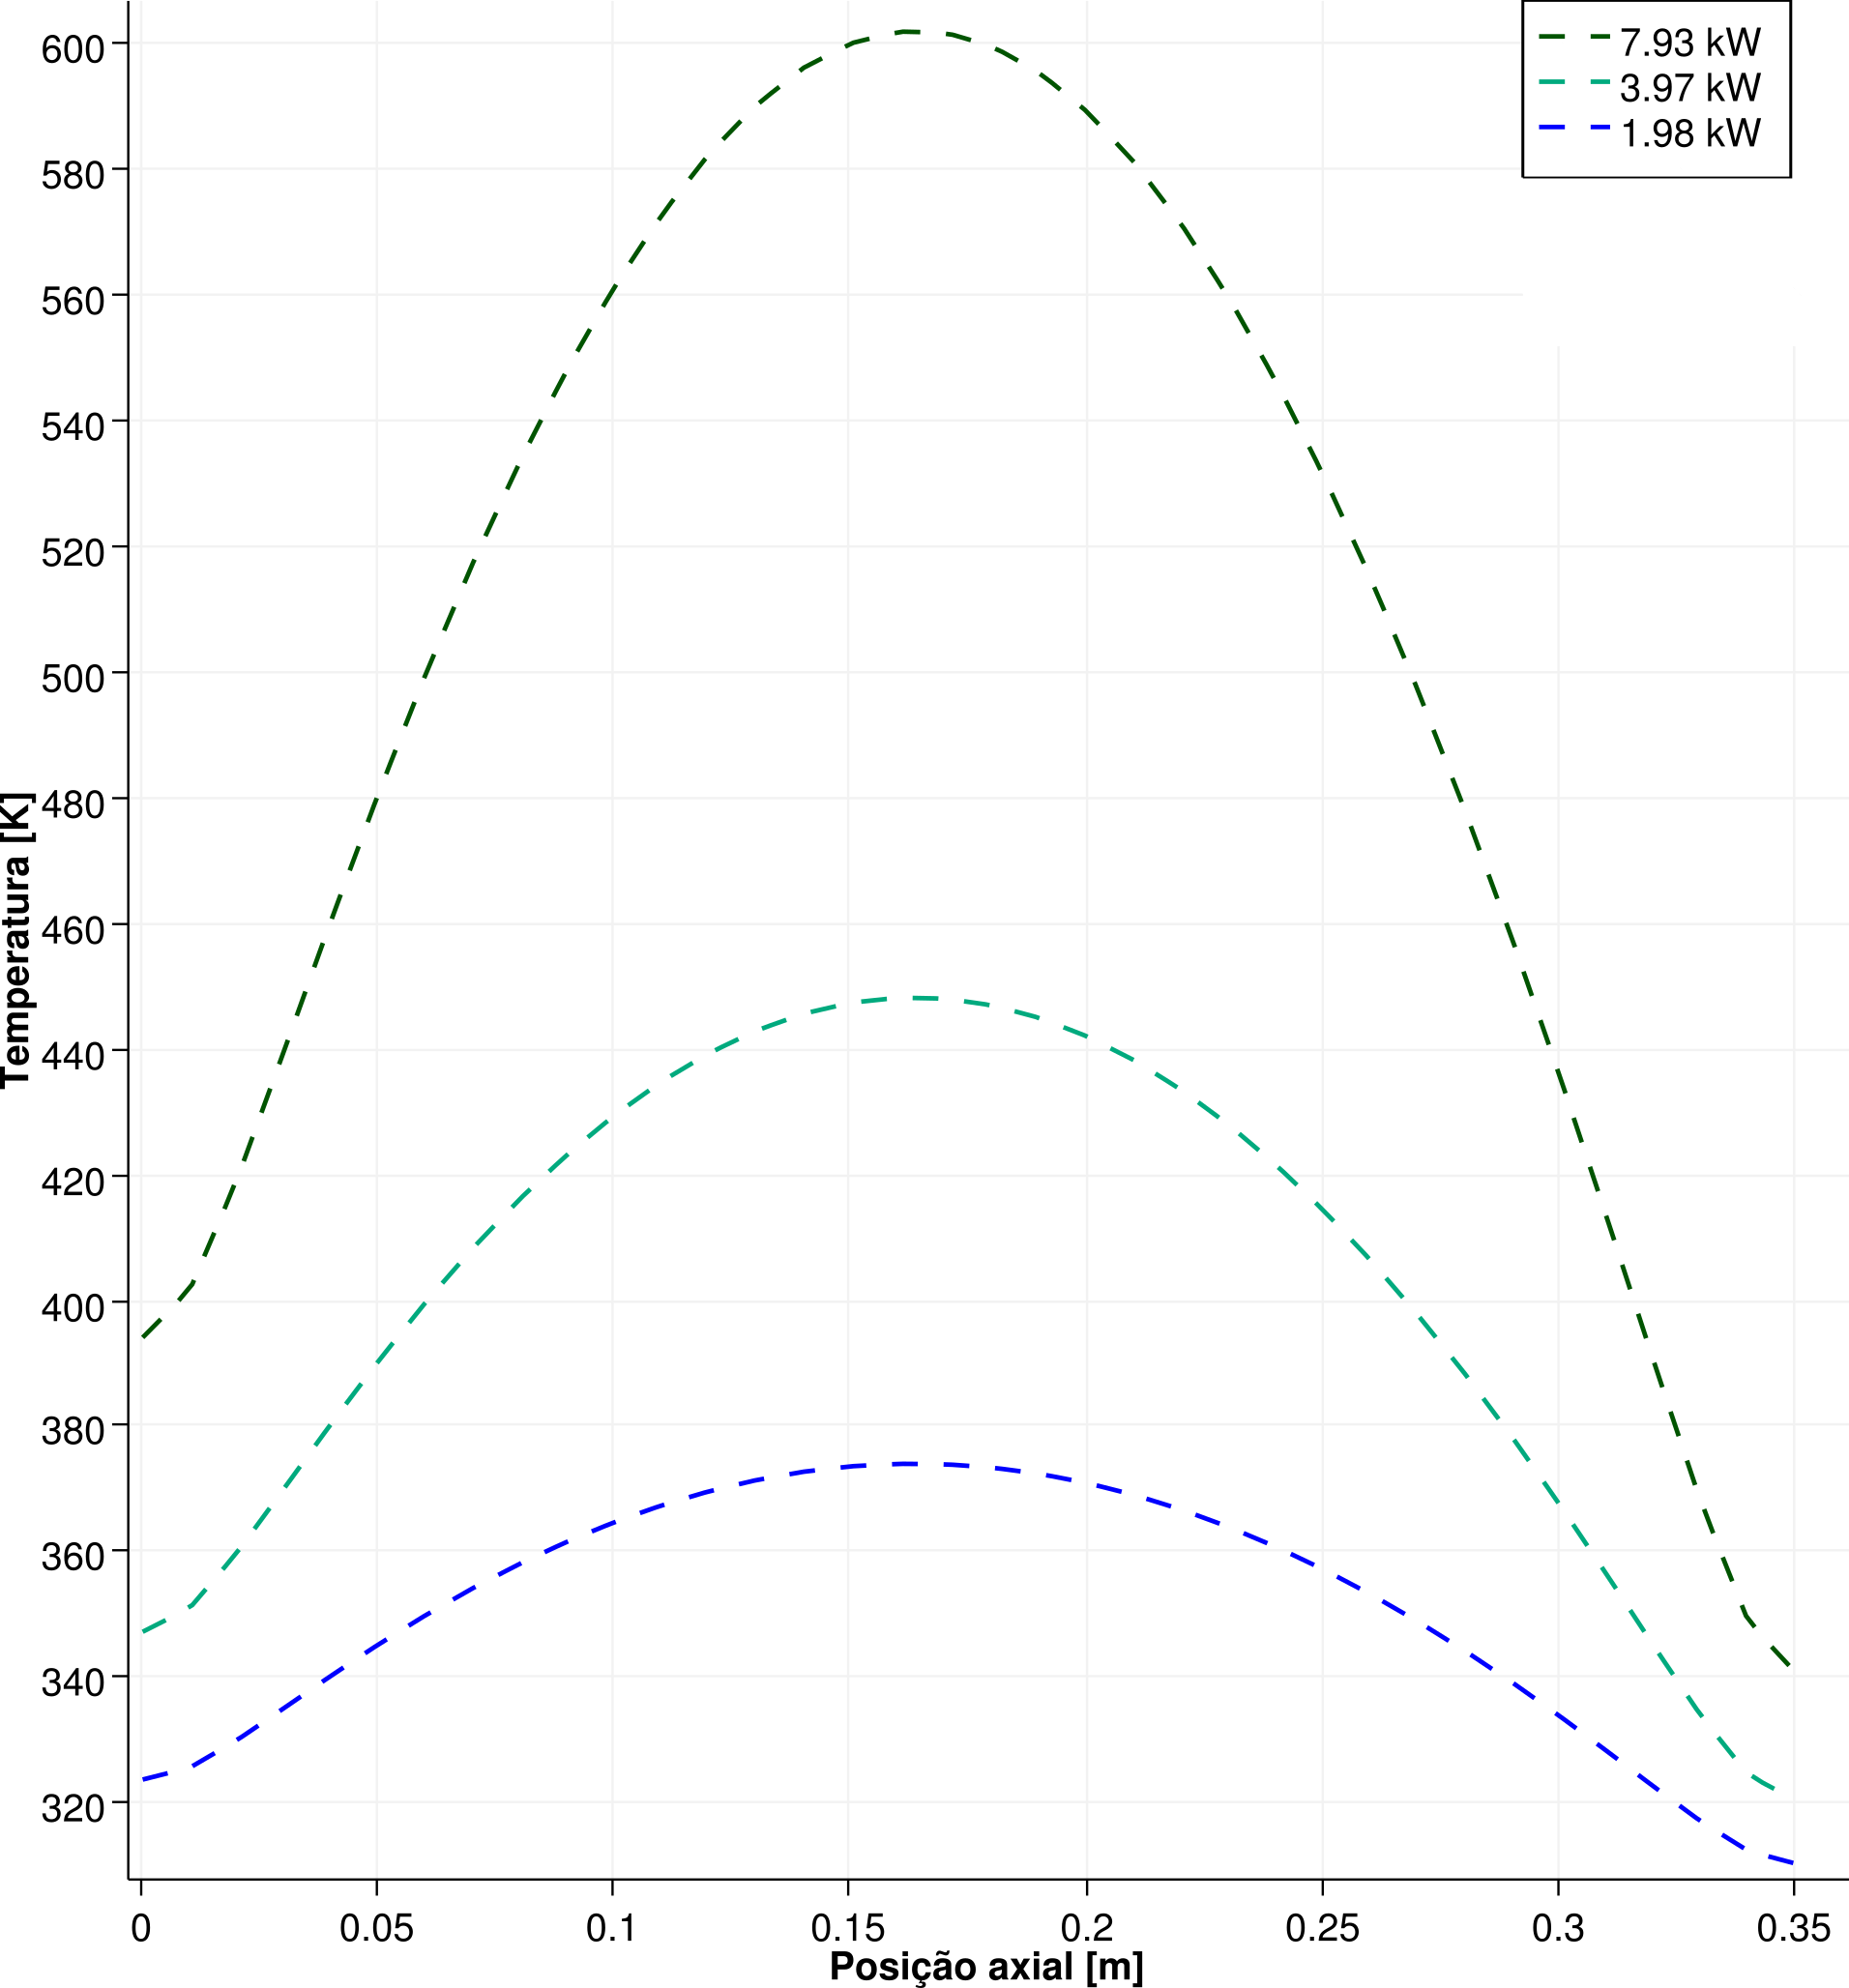
\includegraphics[scale=0.5]{figuras/T_z_NC_square_port.png}
  \label{fig:perf-t-nac-axial}
%  \legend{Fonte: autor}
\end{figure}

Radialmente, os perfis de temperatura, seguindo o mesmo padrão para os três casos simulados,
possuem descontinuidades, como pode ser visto na Figura \ref{fig:perf-t-nac-radial} (entre
$0 m$ e $0,005 m$ e $0,04 m$ e $0,045 m$). Estes degraus indicam mudança no gradiente de temperaturas na
interface entre diferentes materiais, devido às diferentes condutividades térmicas de cada um.
que ocorre no fluxo de calor entre dois materiais com propriedades físicas distintas.

Os resultados das simulações apresentadas para os três casos não-acoplados formam o conjunto de resultados
de referência. Eles servem de base de comparação para as simulações acopladas, com objetivo de verificar
se os resultados acoplados se diferenciam destes e em que medida ocorrem estas diferenças.

\begin{figure}[htb]
  \caption[Perfil de temperaturas radial para os três casos simulados.]
          {Perfil de temperaturas radial para os três casos simulados. No detalhe o perfil de temperatura nas interfaces entre os três materiais.}
  \centering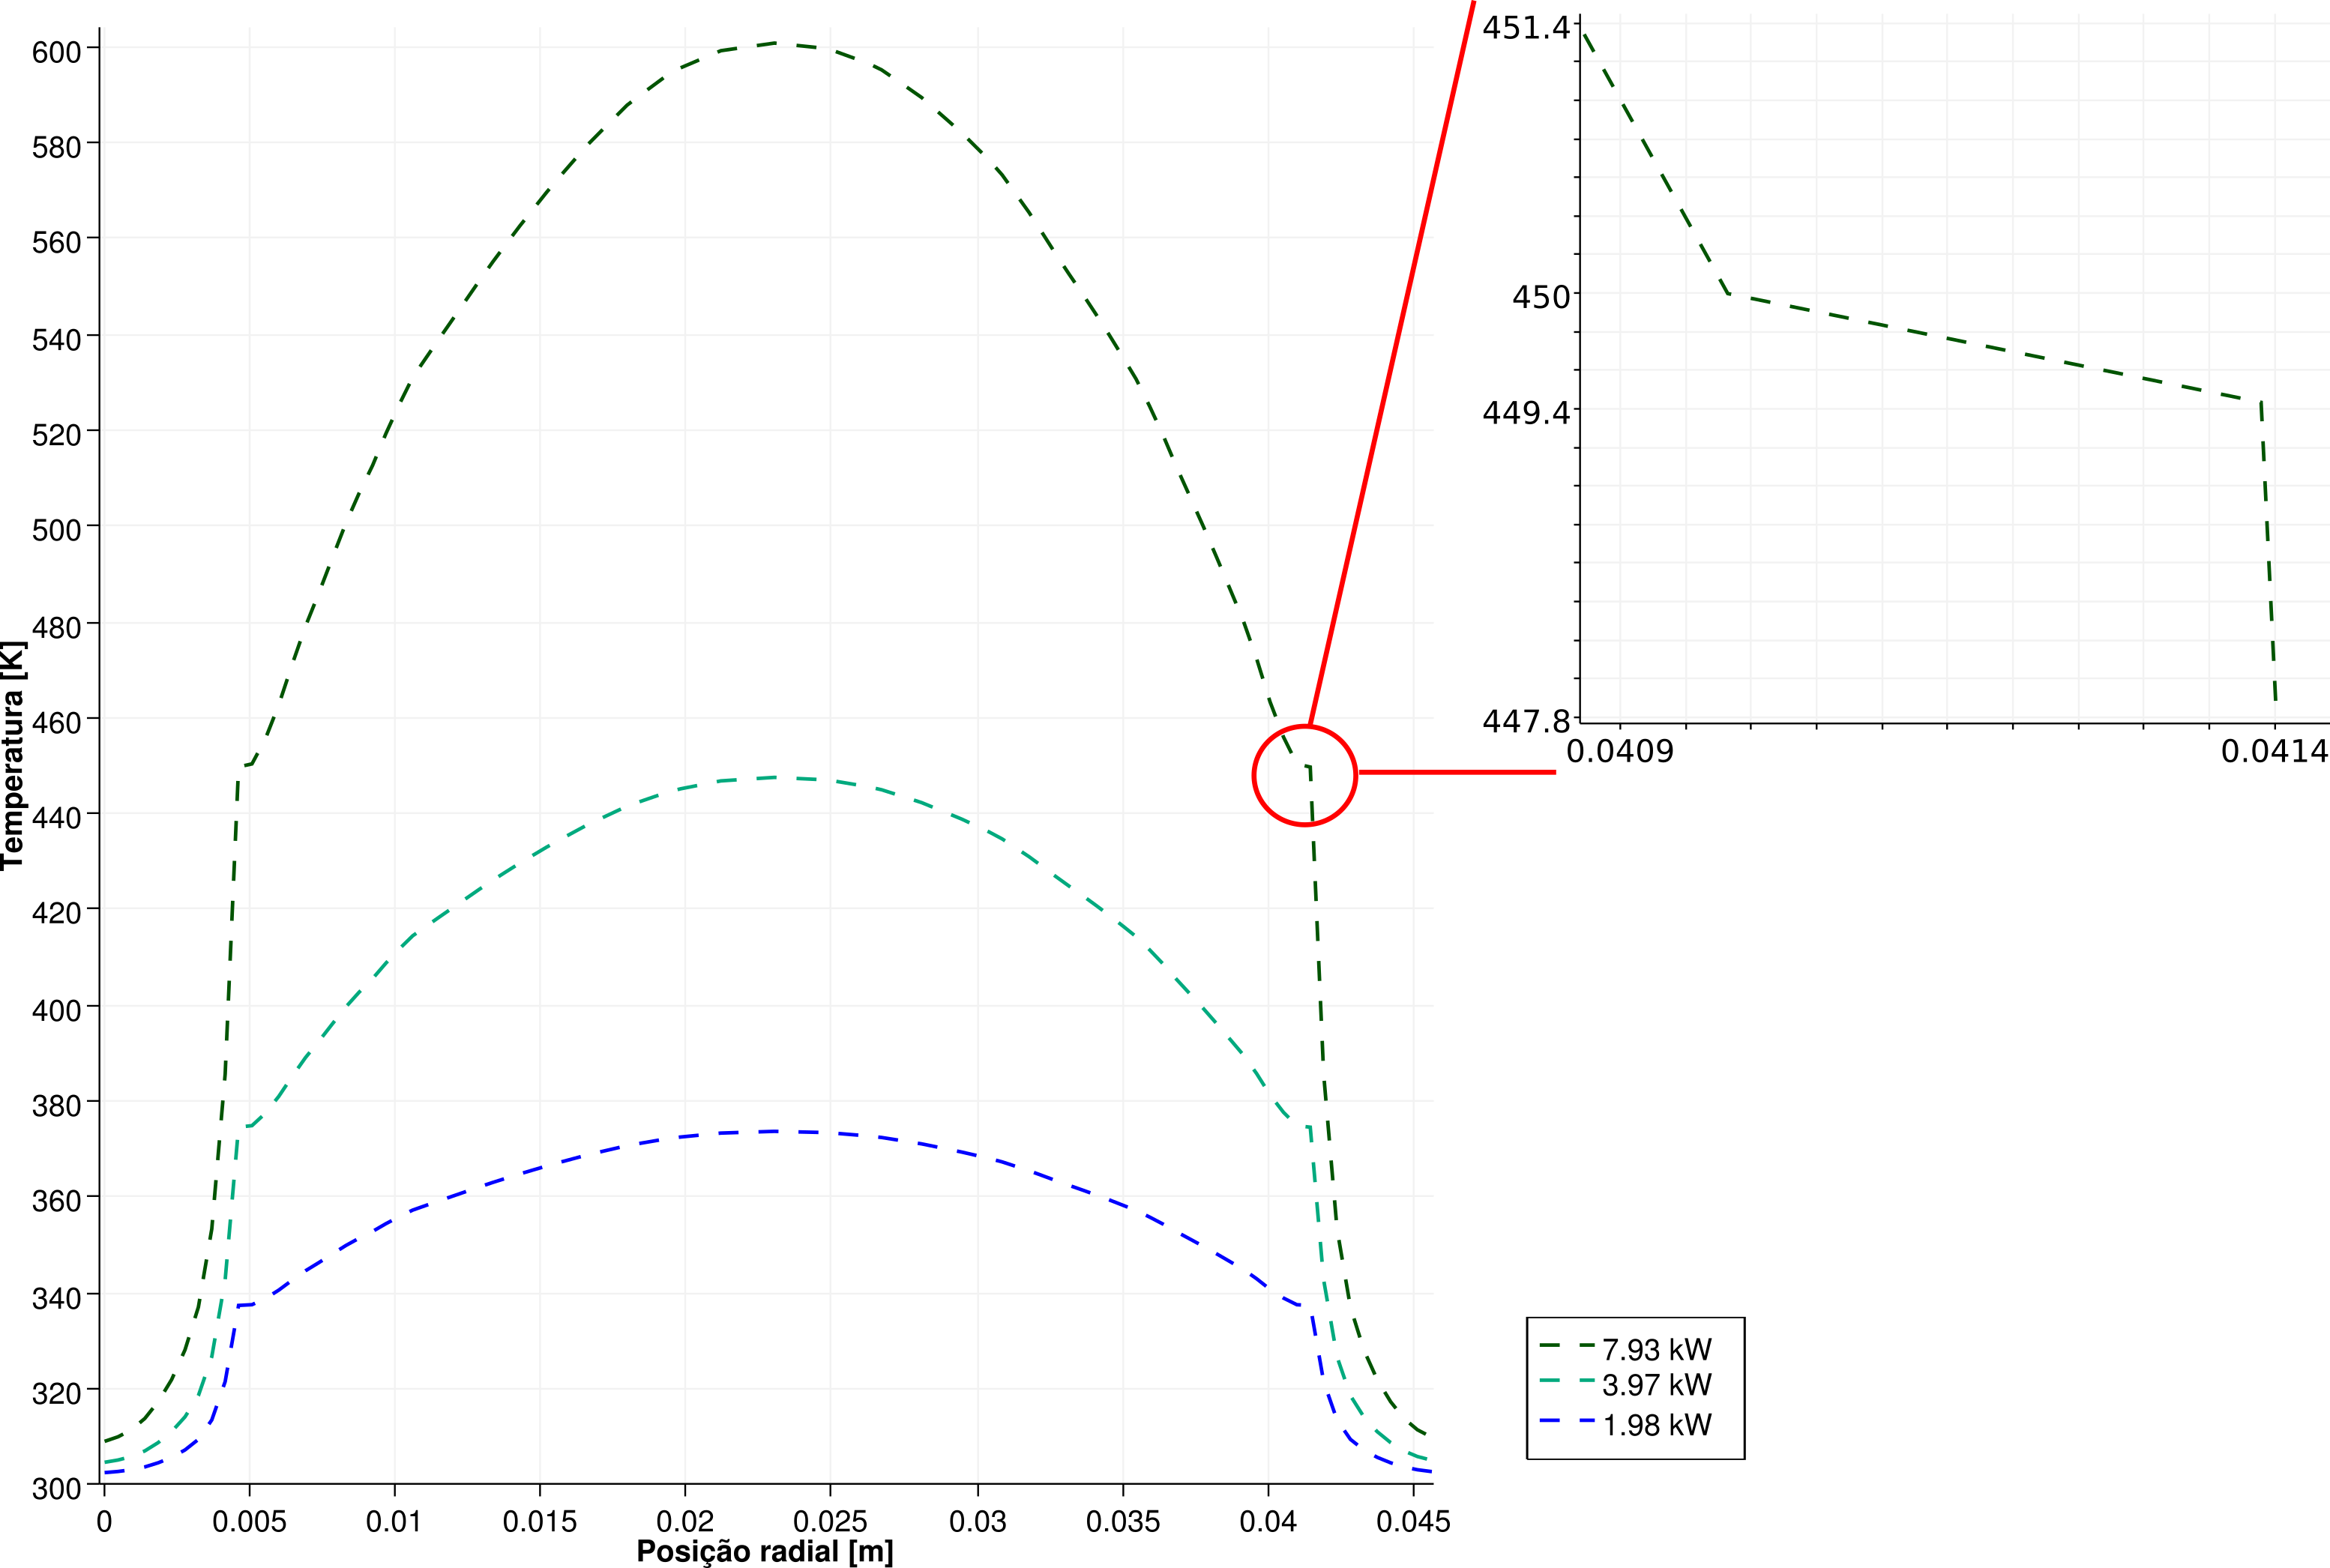
\includegraphics[scale=0.5]{figuras/T_x_NC_square_port_detalhado.png}
  \label{fig:perf-t-nac-radial}
%  \legend{Fonte: autor}
\end{figure}


% ------------------------------------------------------------------------------------------------------------
\section{Caso acoplado}
\label{sec:cp}

As simulações acopladas foram realizadas exatamente nas mesmas condições das suas homólogas não-acopladas.
Os resultados destas são apresentados em comparação com os resultados anteriores para visualização
das diferenças entre elas.

Diferentemente dos cálculos não-acoplados, na simulação acoplada ocorre a variação do fluxo neutrônico.
Essa variação, originada da variação de temperaturas no sistema, ocorre nos três casos acoplados, cada
um simulado numa potência.

Para as simulações a $1,98 kW$, as diferenças no fluxo são as mais sutis. Com potência mais baixa, há menor
diferença nas temperaturas entre o caso acoplado e o não-acoplado. Como as seções de choque variam de
acordo com a temperatura, é menor a diferença entre seções de choque. Por consequência, menor a diferença
no fluxo neutrônico. Outro fator que leva à similaridade entre os fluxos é a baixa granularidade
da malha na direção axial (apenas 35 camadas de elementos, como apresentado na Tabela \ref{tab:size_model}).

Na Figura \ref{fig:flux_z_50} são apresentados os fluxos axiais acoplados e não acoplados nas simulações
à potência mais baixa, de $1,98 kW$. A diferença entre os fluxos é melhor percebida no corte radial,
apresentado na Figura \ref{fig:flux_x_50}. Além de uma maior variação radial devido à moderação de nêutrons
nas paredes, e consequente aumento do fluxo térmico, a malha é radialmente mais refinada. Com isso, é possível
captar mais detalhes do fluxo neutrônico.

%Ver se dá pra colocar tempo e parâmetros de convergência.

\begin{figure}[htb]
  \caption{Fluxos relativos axiais entre simulação acoplada e não acoplada para
    potência de 1,98 kW.}
  \centering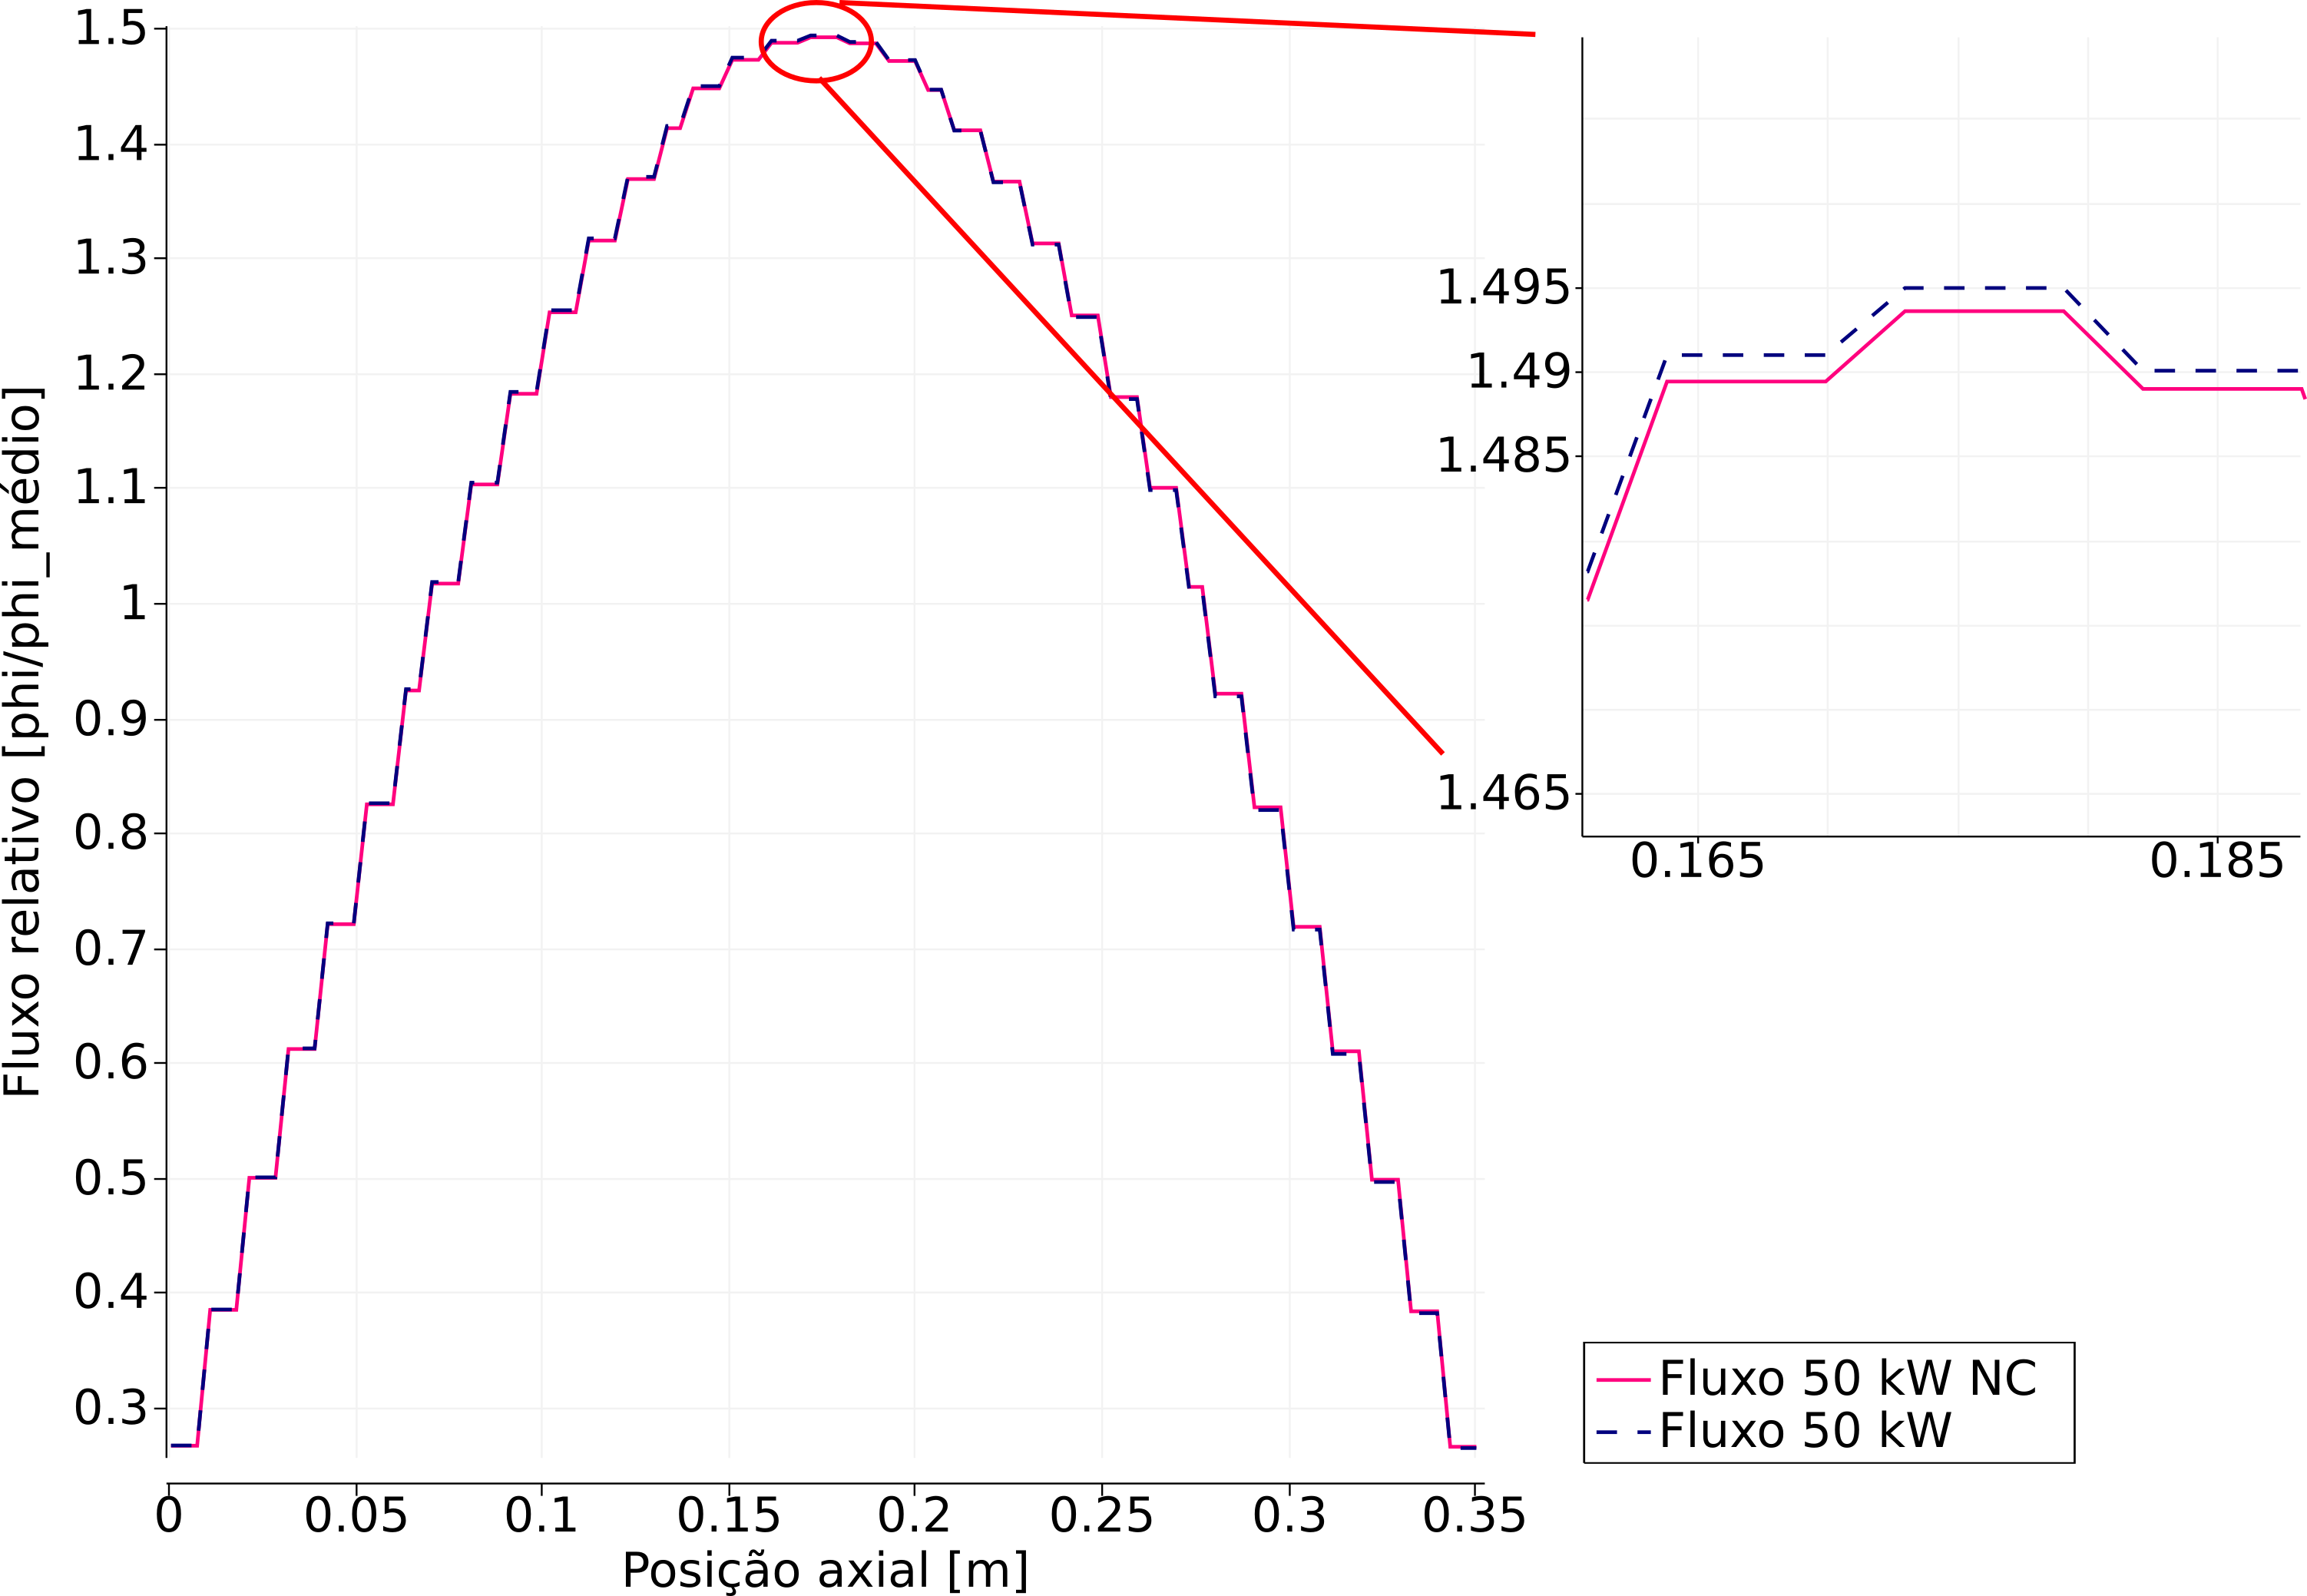
\includegraphics[scale=0.5]{figuras/Flux_rel_z_50_port_trabalhado.png}
  \label{fig:flux_z_50}
%  \legend{Fonte: autor}
\end{figure}

\begin{figure}[htb]
  \caption{Fluxos relativos radiais entre simulação acoplada e não acoplada para
    potência de 1,98 kW.}
  \centering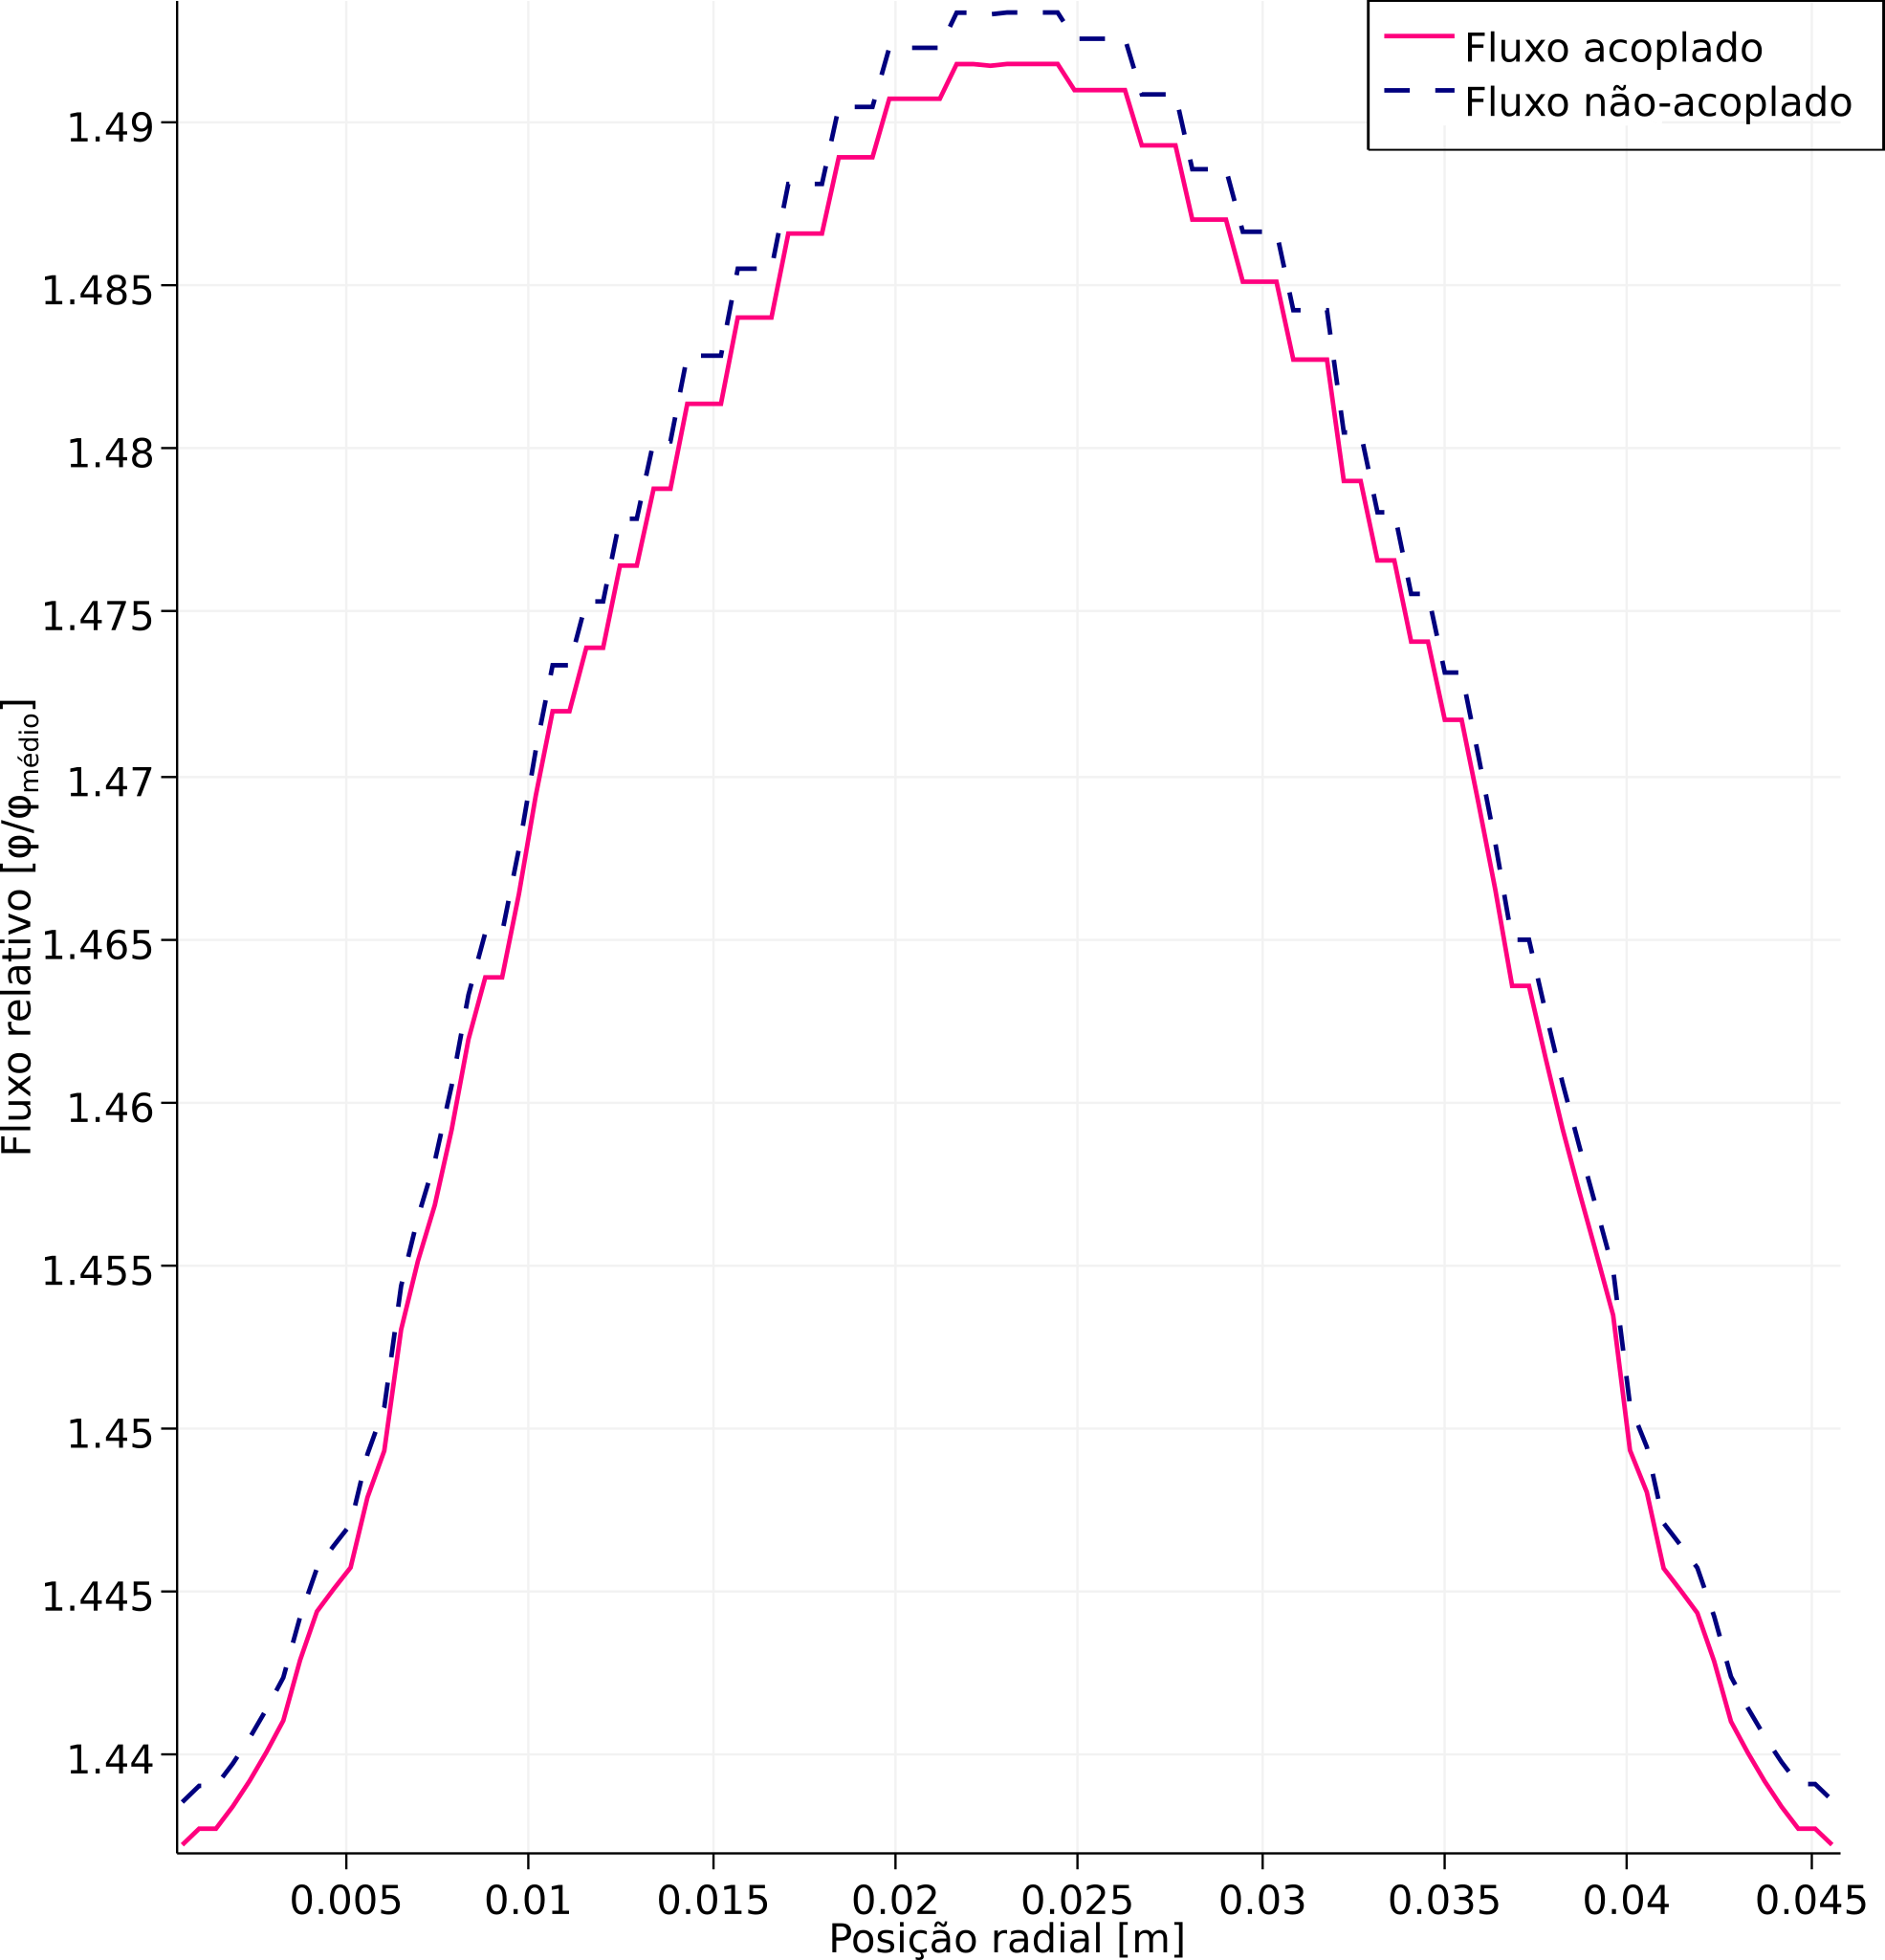
\includegraphics[scale=0.5]{figuras/Flux_rel_x_50_port.png}
  \label{fig:flux_x_50}
%  \legend{Fonte: autor}
\end{figure}

As mesmas observações feitas para os fluxos relativos na menor potência são válidas
para as simulações feitas à potência de $3,97 kW$. Novamente, as diferenças entre
os fluxos relativos são melhor observáveis no corte radial do que no corte axial.
Entretanto, as diferenças entre os fluxo começam a aumentar de acordo com o
aumento da potência. Os fluxos relativos axiais acoplados e não-acoplados para
potência de $3,97 kW$ podem ser observados na Figura \ref{fig:flux_z_100}, enquanto
os fluxos relativos radiais para a mesma potência podem ser observados na Figura \ref{fig:flux_x_100}.

\begin{figure}[htb]
  \caption{Fluxos relativos axiais entre simulação acoplada e não acoplada para
    potência de 3,97 kW.}
  \centering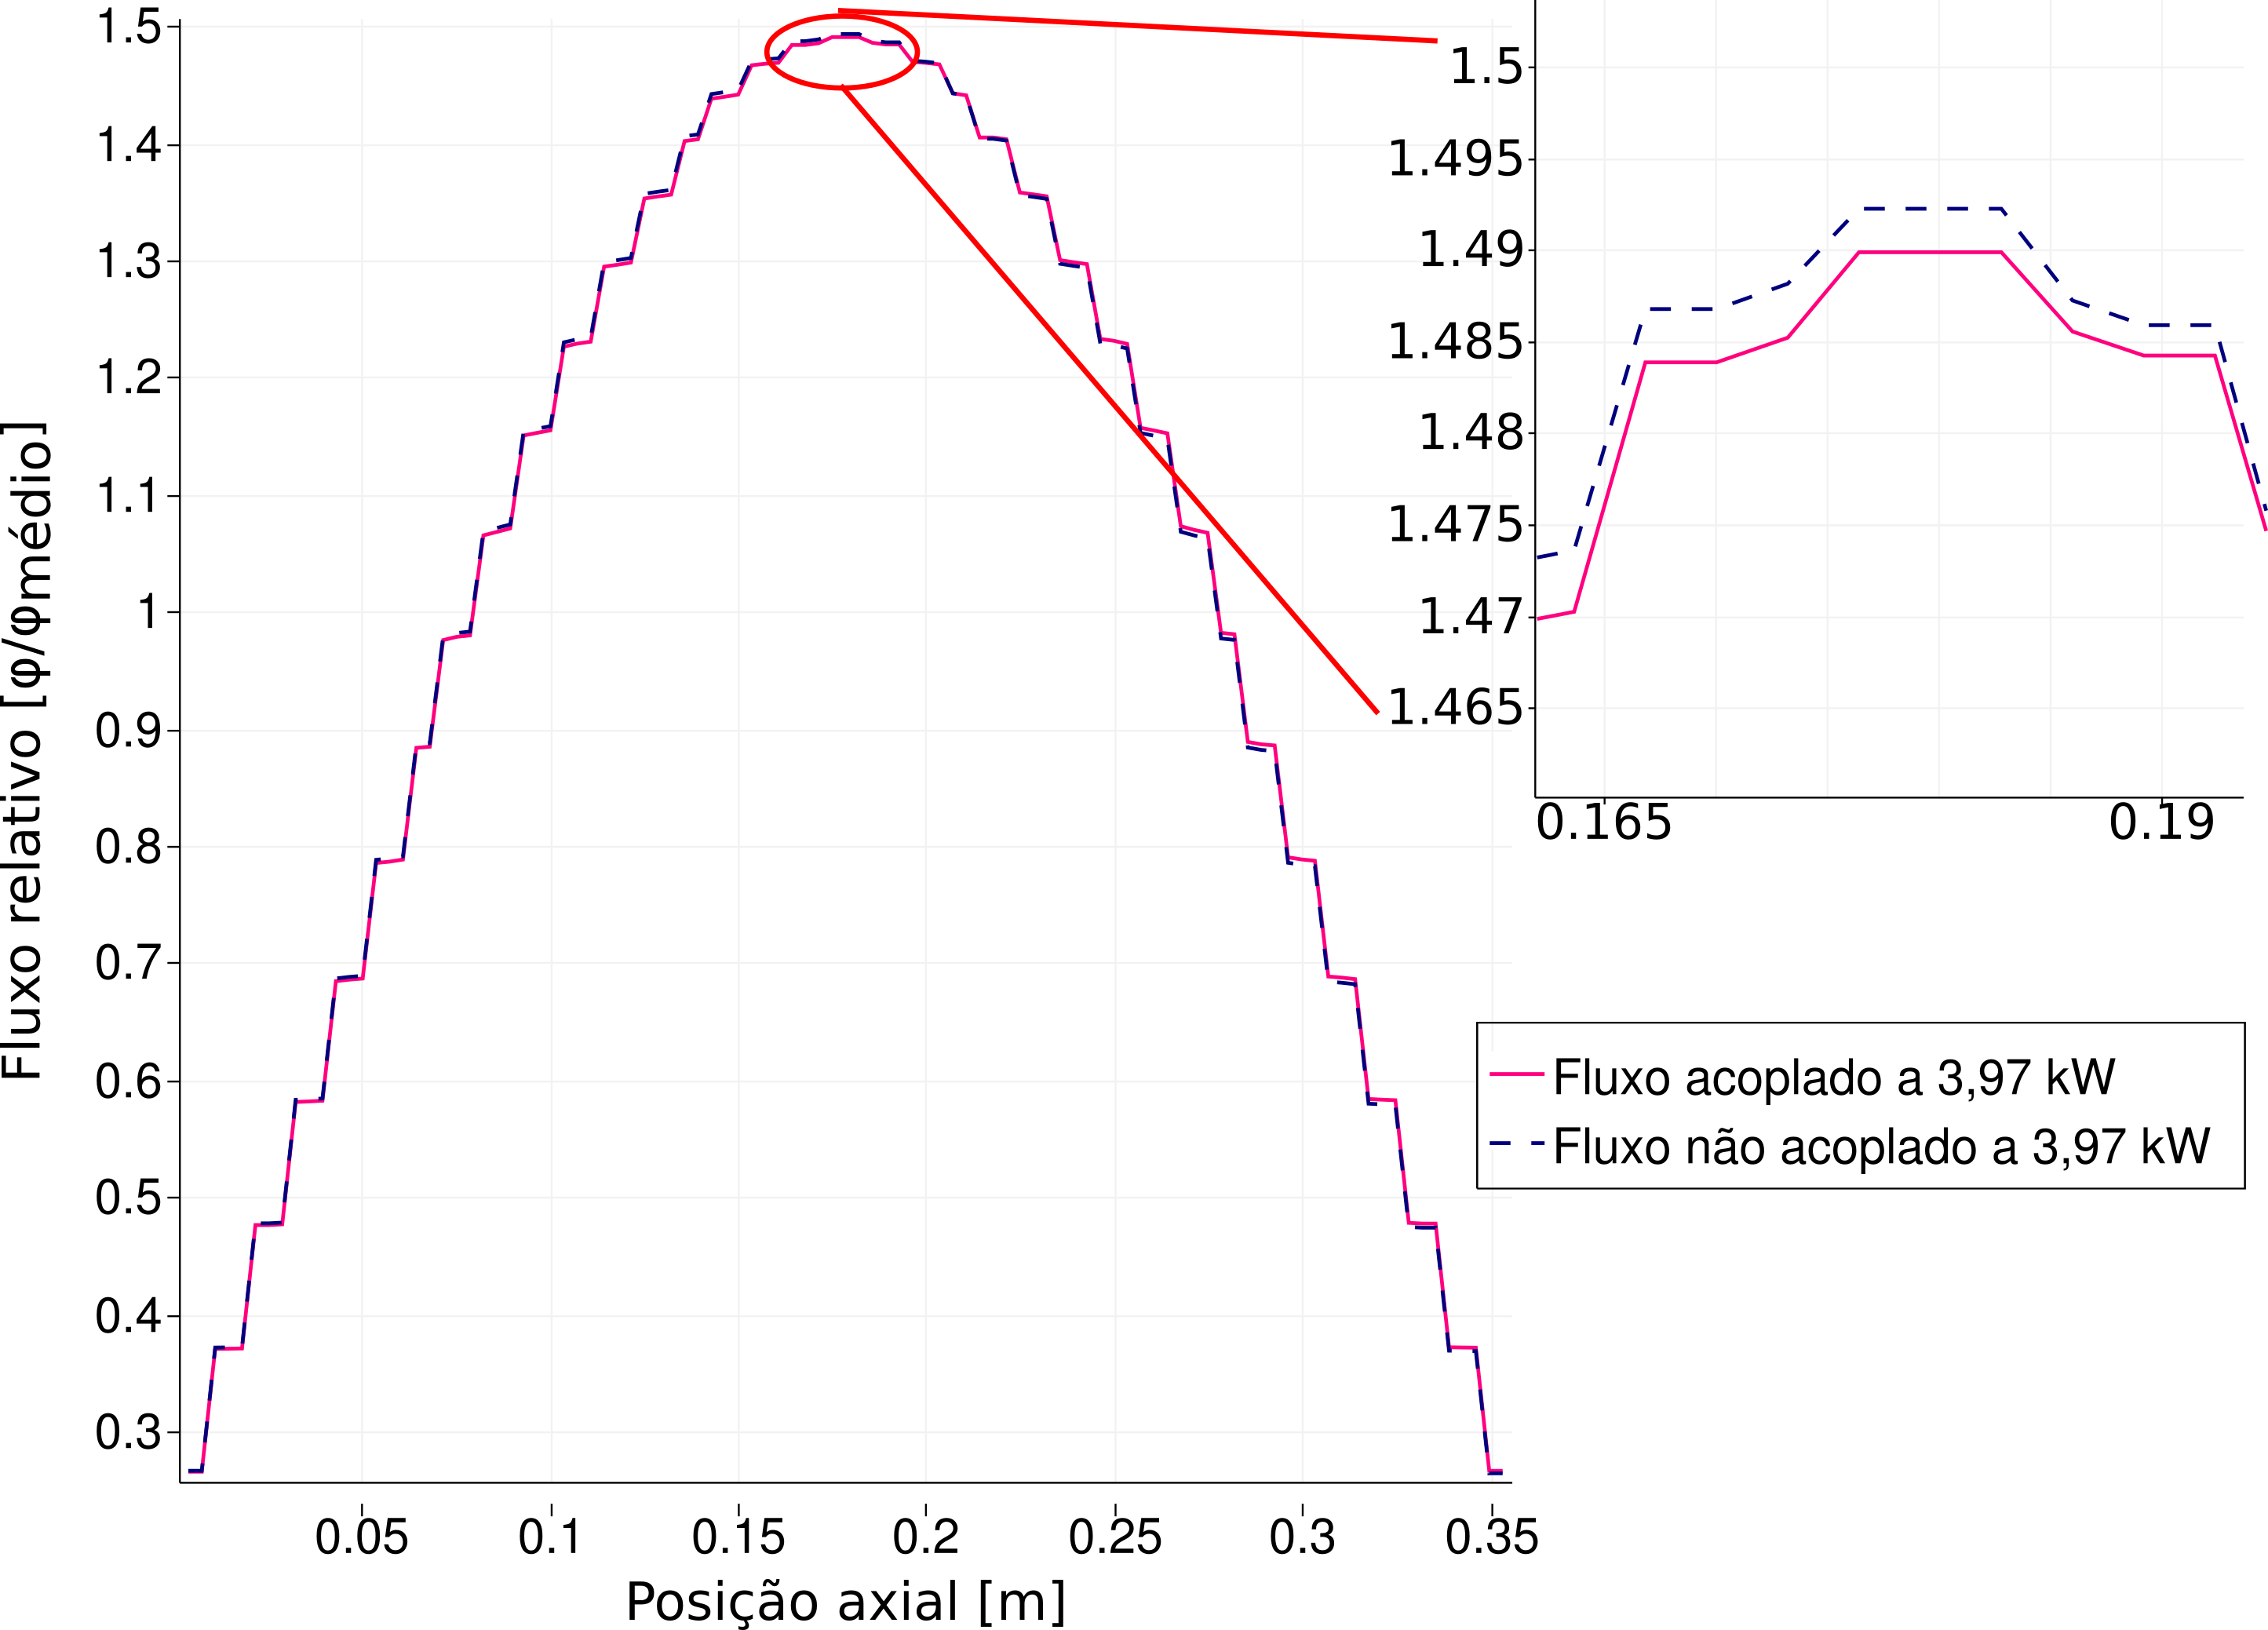
\includegraphics[scale=0.5]{figuras/Flux_rel_z_100_port_trabalhado.png}
  \label{fig:flux_z_100}
%  \legend{Fonte: autor}
\end{figure}

\begin{figure}[htb]
  \caption{Fluxos relativos radiais entre simulação acoplada e não acoplada para
    potência de 3,97 kW.}
  \centering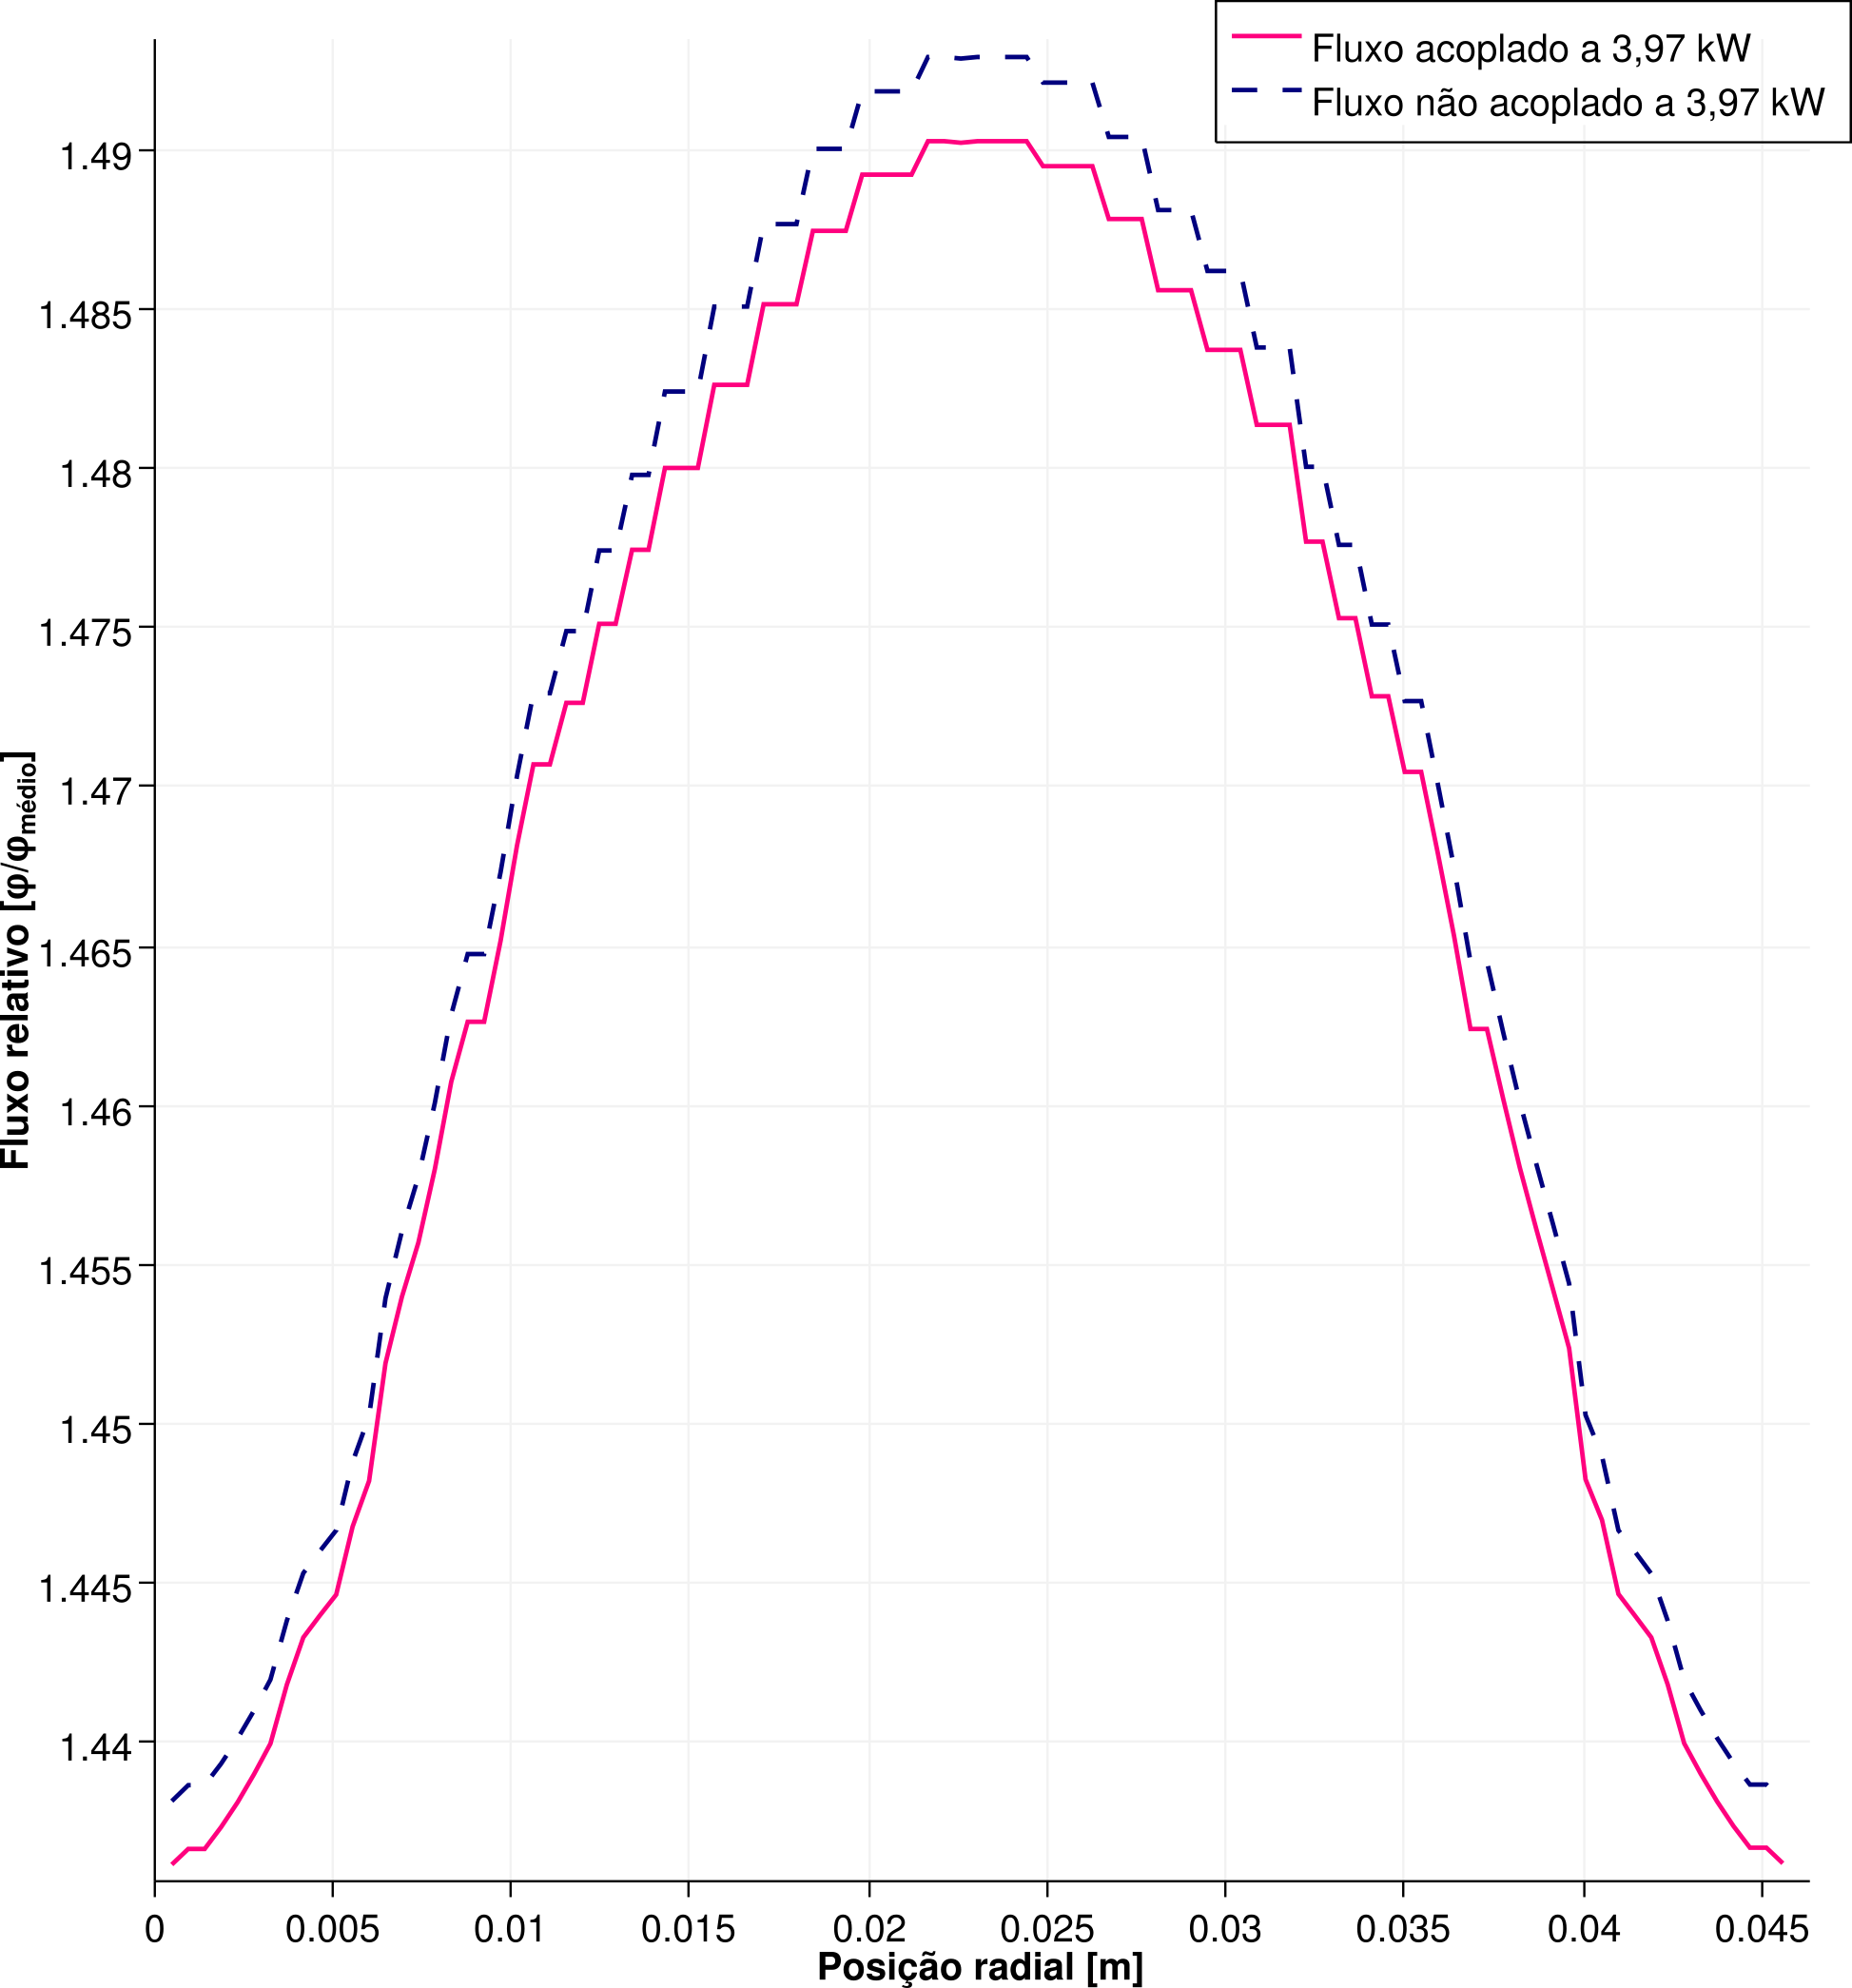
\includegraphics[scale=0.5]{figuras/Flux_rel_x_100_port.png}
  \label{fig:flux_x_100}
%  \legend{Fonte: autor}
\end{figure}

As diferenças entre os fluxos relativos em ambas as simulações passa a ser melhor
vista nas simulações de maior potência, a $7,93 kW$. Novamente, a variação nas temperaturas
impacta nos cálculos acoplados, uma vez que as seções de choque são periodicamente
recalculadas. É possível observar na Figura \ref{fig:flux_z_200}, que apresenta o perfil axial,
uma sutil sobreposição entre as curvas, demonstrando um achatamento na curva
referente as cálculos acoplados. Isso se explica pelas propriedades do combustível modelado,
que diminui sua capacidade de absorção de nêutrons térmicos com o aumento da temperatura.
Ao mesmo tempo, nas extremidades da curva, as temperaturas são menores que no caso não-acoplado,
levando a um relativo aumento no fluxo. O fluxo acoplado reflete tais mudanças no seu perfil.

As diferenças entre os fluxos relativos radiais, para a potência de $7,93 kW$, são facilmente
visíveis na Figura \ref{fig:flux_x_200}.

\begin{figure}[htb]
  \caption{Fluxos relativos axiais entre simulação acoplada e não acoplada para
    potência de 7,93 kW.}
  \centering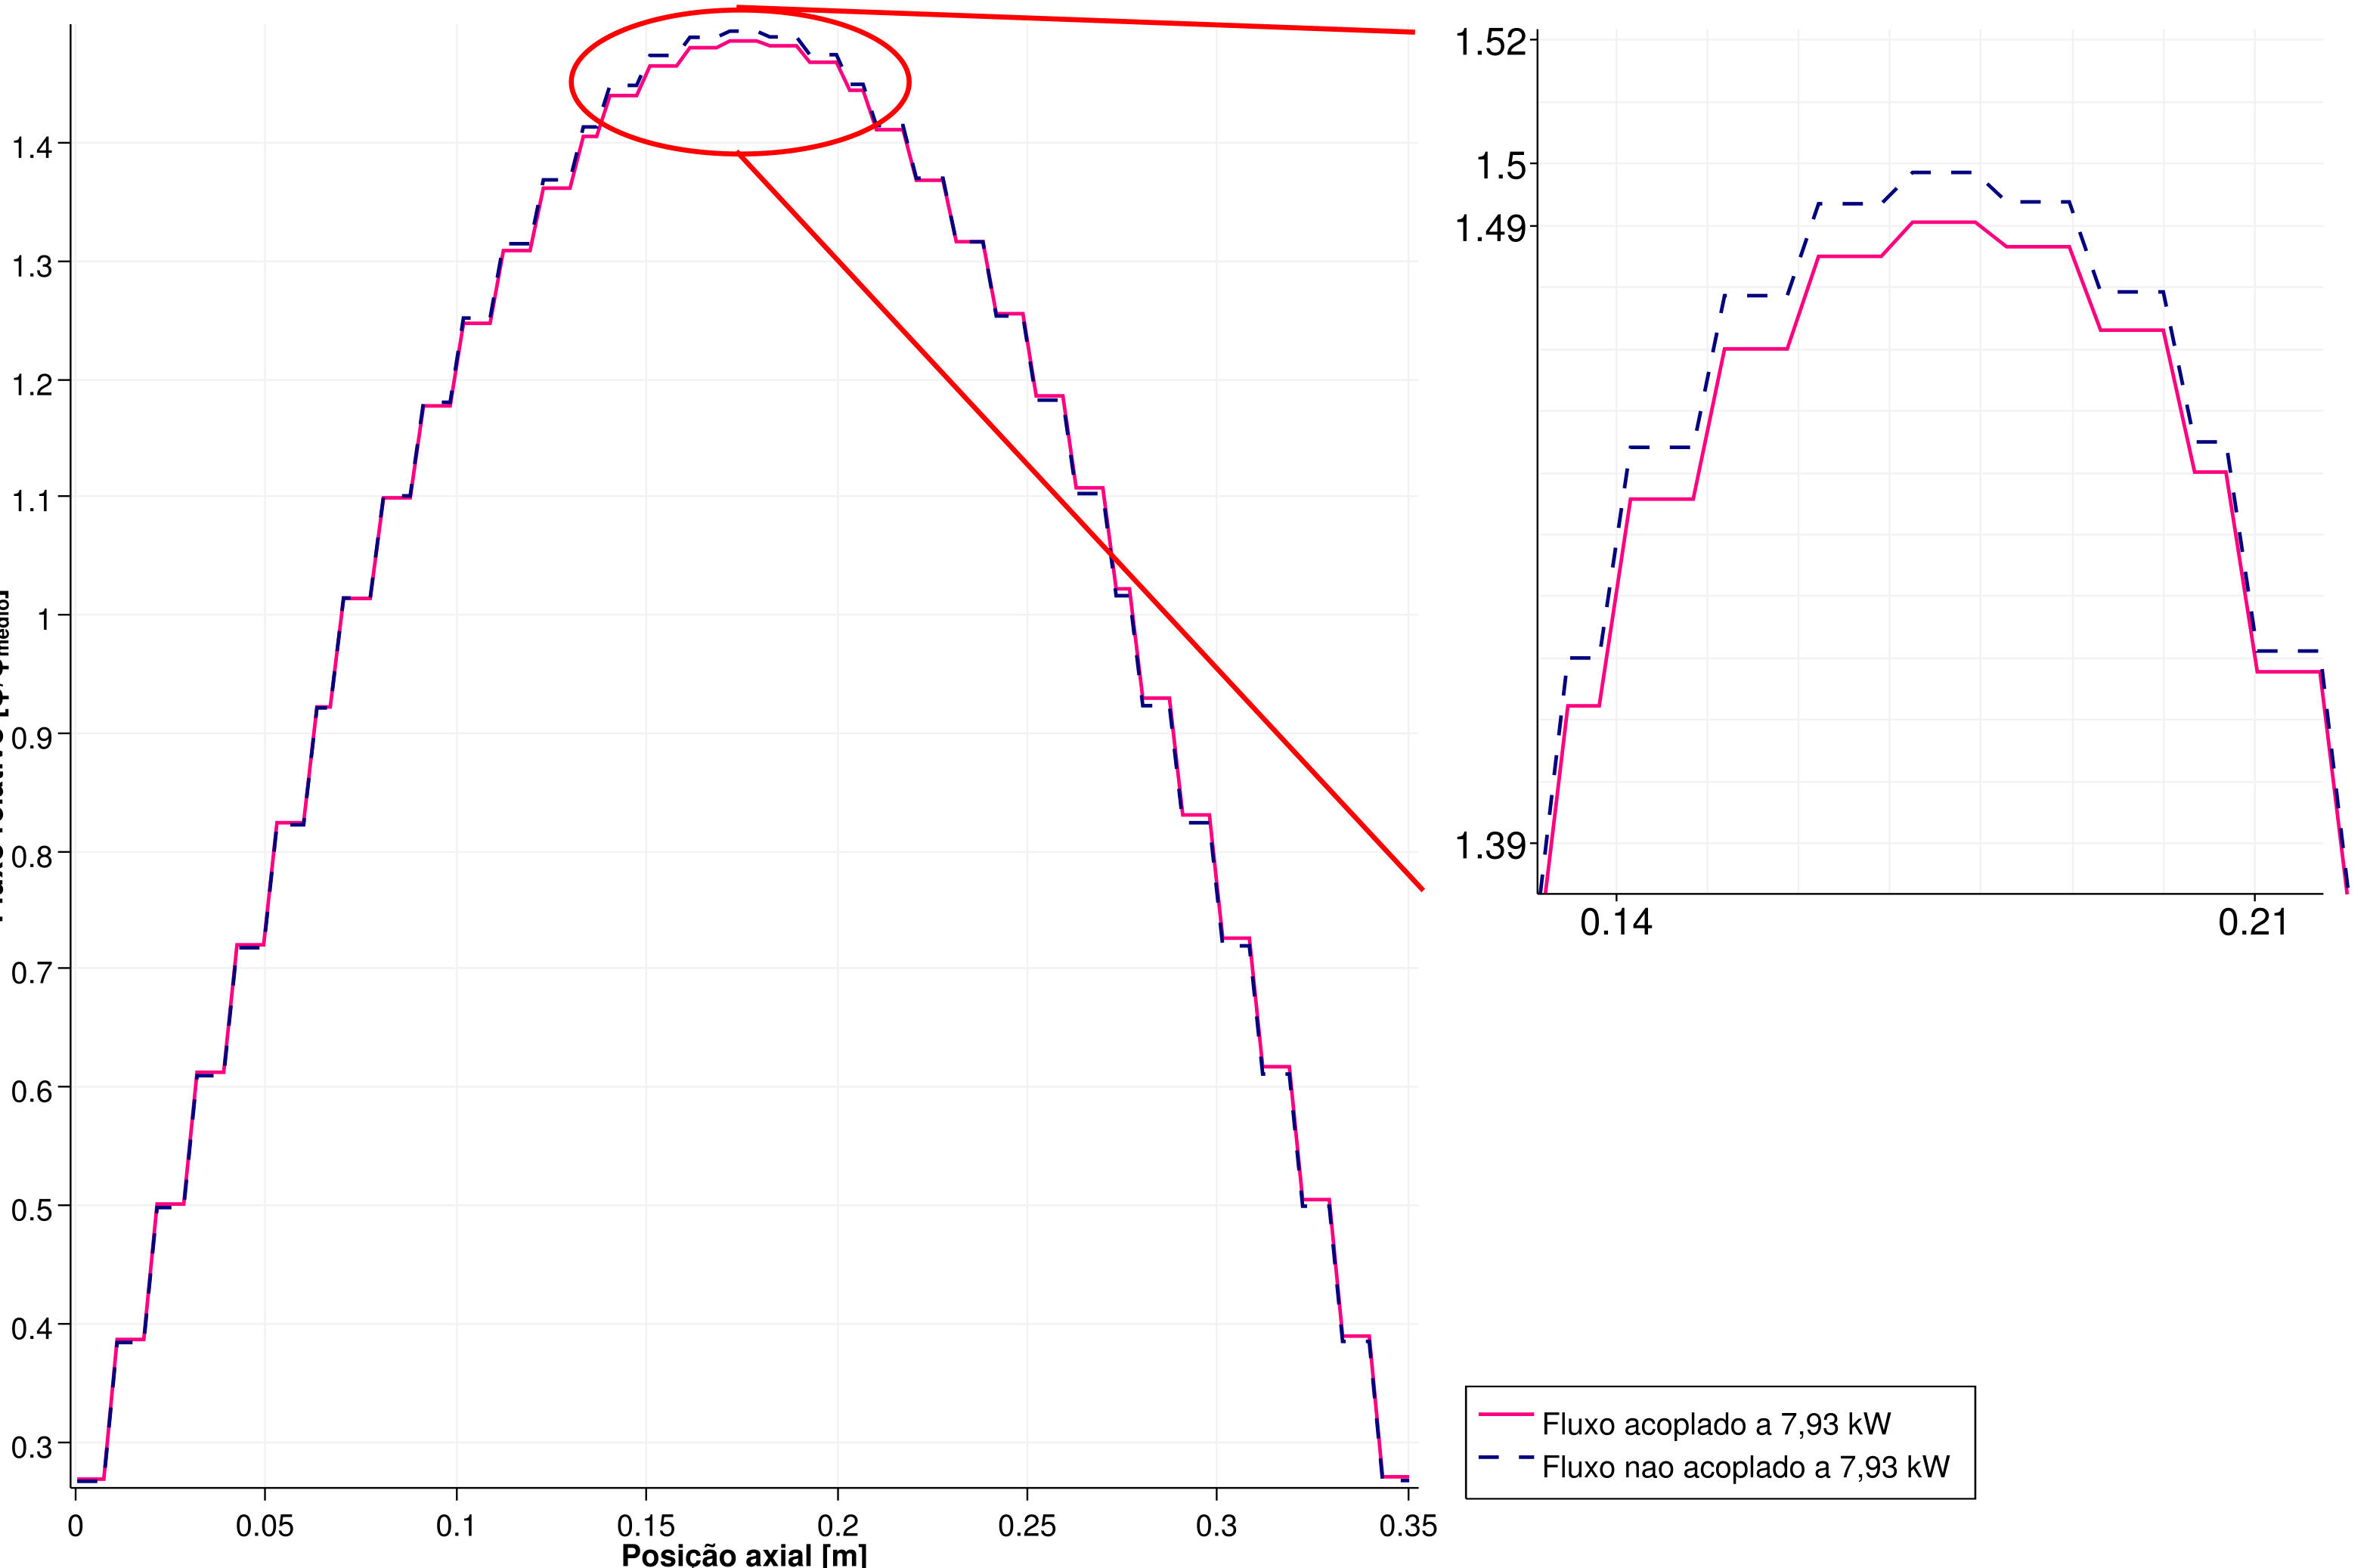
\includegraphics[scale=0.5]{figuras/Flux_rel_z_200_port_trabalhado.png}
  \label{fig:flux_z_200}
%  \legend{Fonte: autor}
\end{figure}

\begin{figure}[htb]
  \caption{Fluxos relativos radiais entre simulação acoplada e não acoplada para
    potência de 7,93 kW.}
  \centering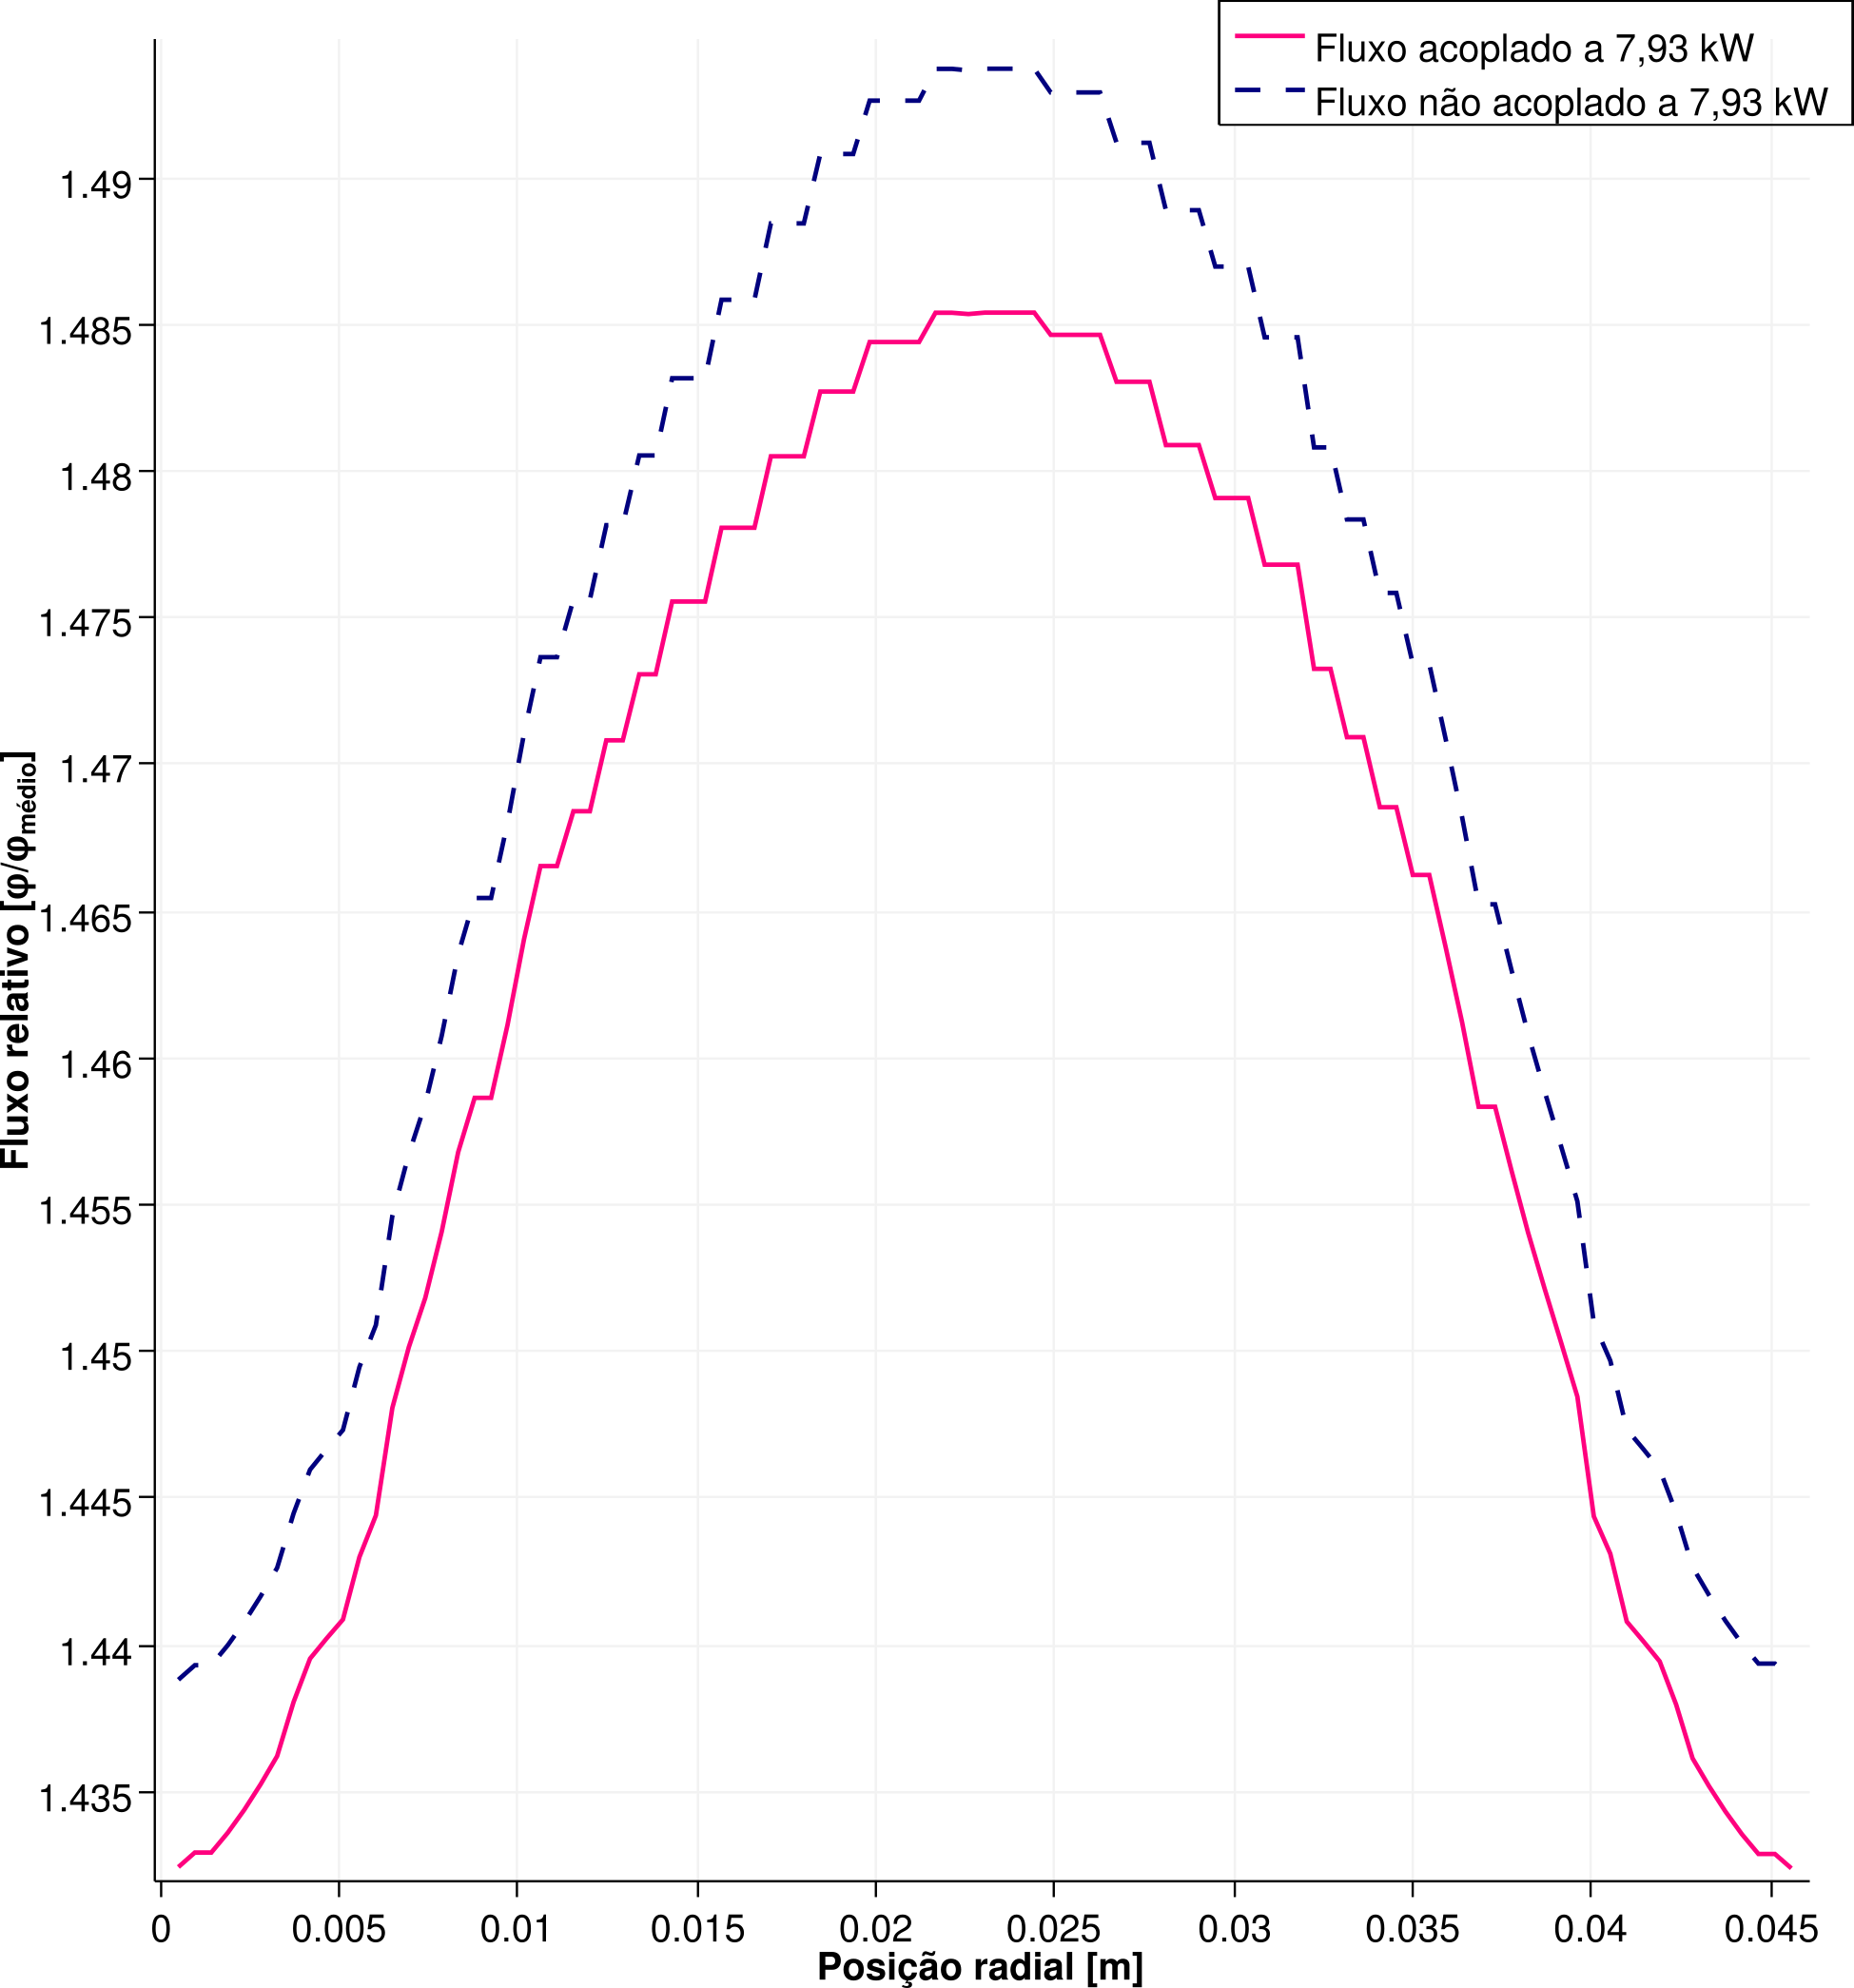
\includegraphics[scale=0.5]{figuras/Flux_rel_x_200_port.png}
  \label{fig:flux_x_200}
%  \legend{Fonte: autor}
\end{figure}

As diferenças entre os fluxos calculados de forma acoplada e não-acoplada ocorrem,
como é de se esperar, nos perfis de potência. A potência não é calculada pela
neutrônica. A solução da aproximação por difusão é o fluxo neutrônico e, a partir
dele, é calculada a potência volumétrica a partir de um valor de referência para
a potência.

É a potência\footnote{A palavra potência é indistintamente utilizada neste capítulo como potência
  propriamente dita, em $W$ ou como sinônimo de potência volumétrica, dada em $W/m^3$, de acordo
com o contexto em que é usada.} que leva ao aquecimento dos materiais que, por sua vez, impactam
no cálculos de seções de choque. As diferenças entre os perfis de potência obtidos nos dois conjuntos
de simulações, acopladas e não-acopladas, são apresentados nas Figuras \ref{fig:Q_all_z} e
\ref{fig:Q_all_x} respectivamente nas direções axial e radial. Observando estas Figuras,
é possível perceber que as diferenças em potência entre os casos acoplados e
não acoplados aumenta de acordo com o aumento da potência.

Cabe comentar que, além das diferenças em valores, há mudanças no formato das curvas.


\begin{figure}[htb]
  \caption{Curvas de potência axiais para os casos acoplados e não acoplados.}
  \centering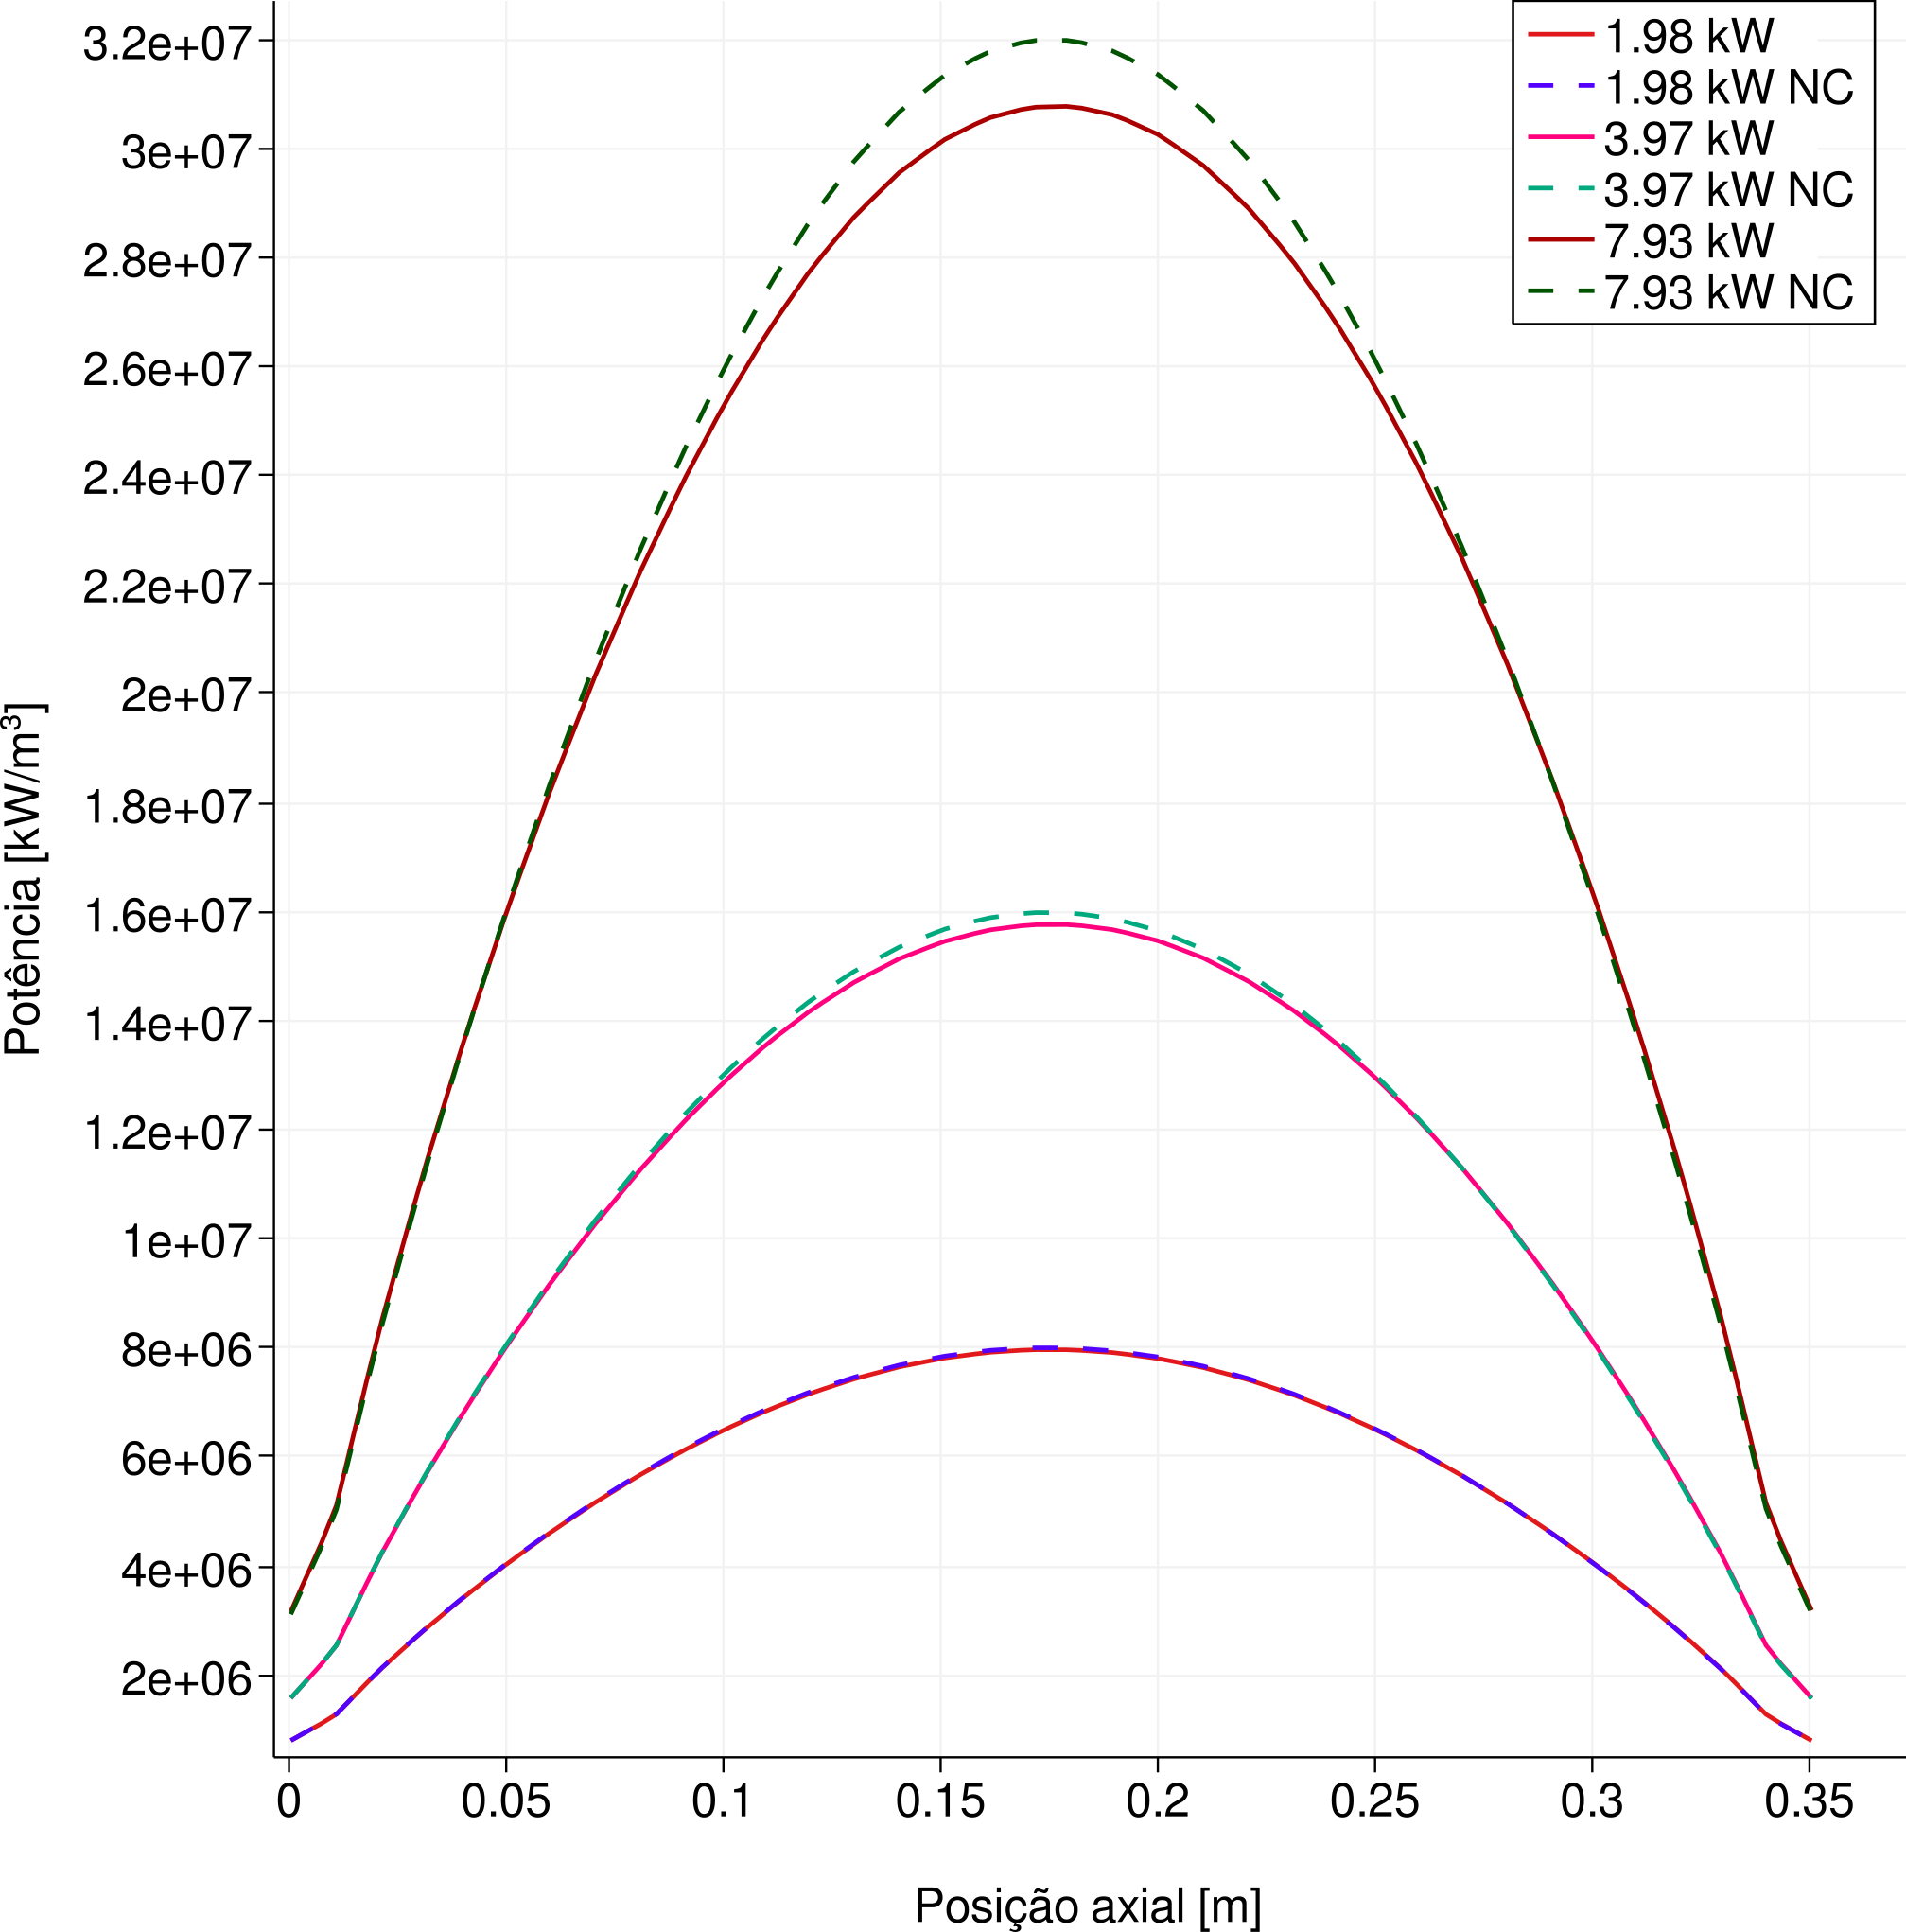
\includegraphics[scale=0.5]{figuras/Q_all_z_square_port.png}
  \label{fig:Q_all_z}
%  \legend{Fonte: autor}
\end{figure}

\begin{figure}[htb]
  \caption{Curvas de potência axiais para os casos acoplados e não acoplados.}
  \centering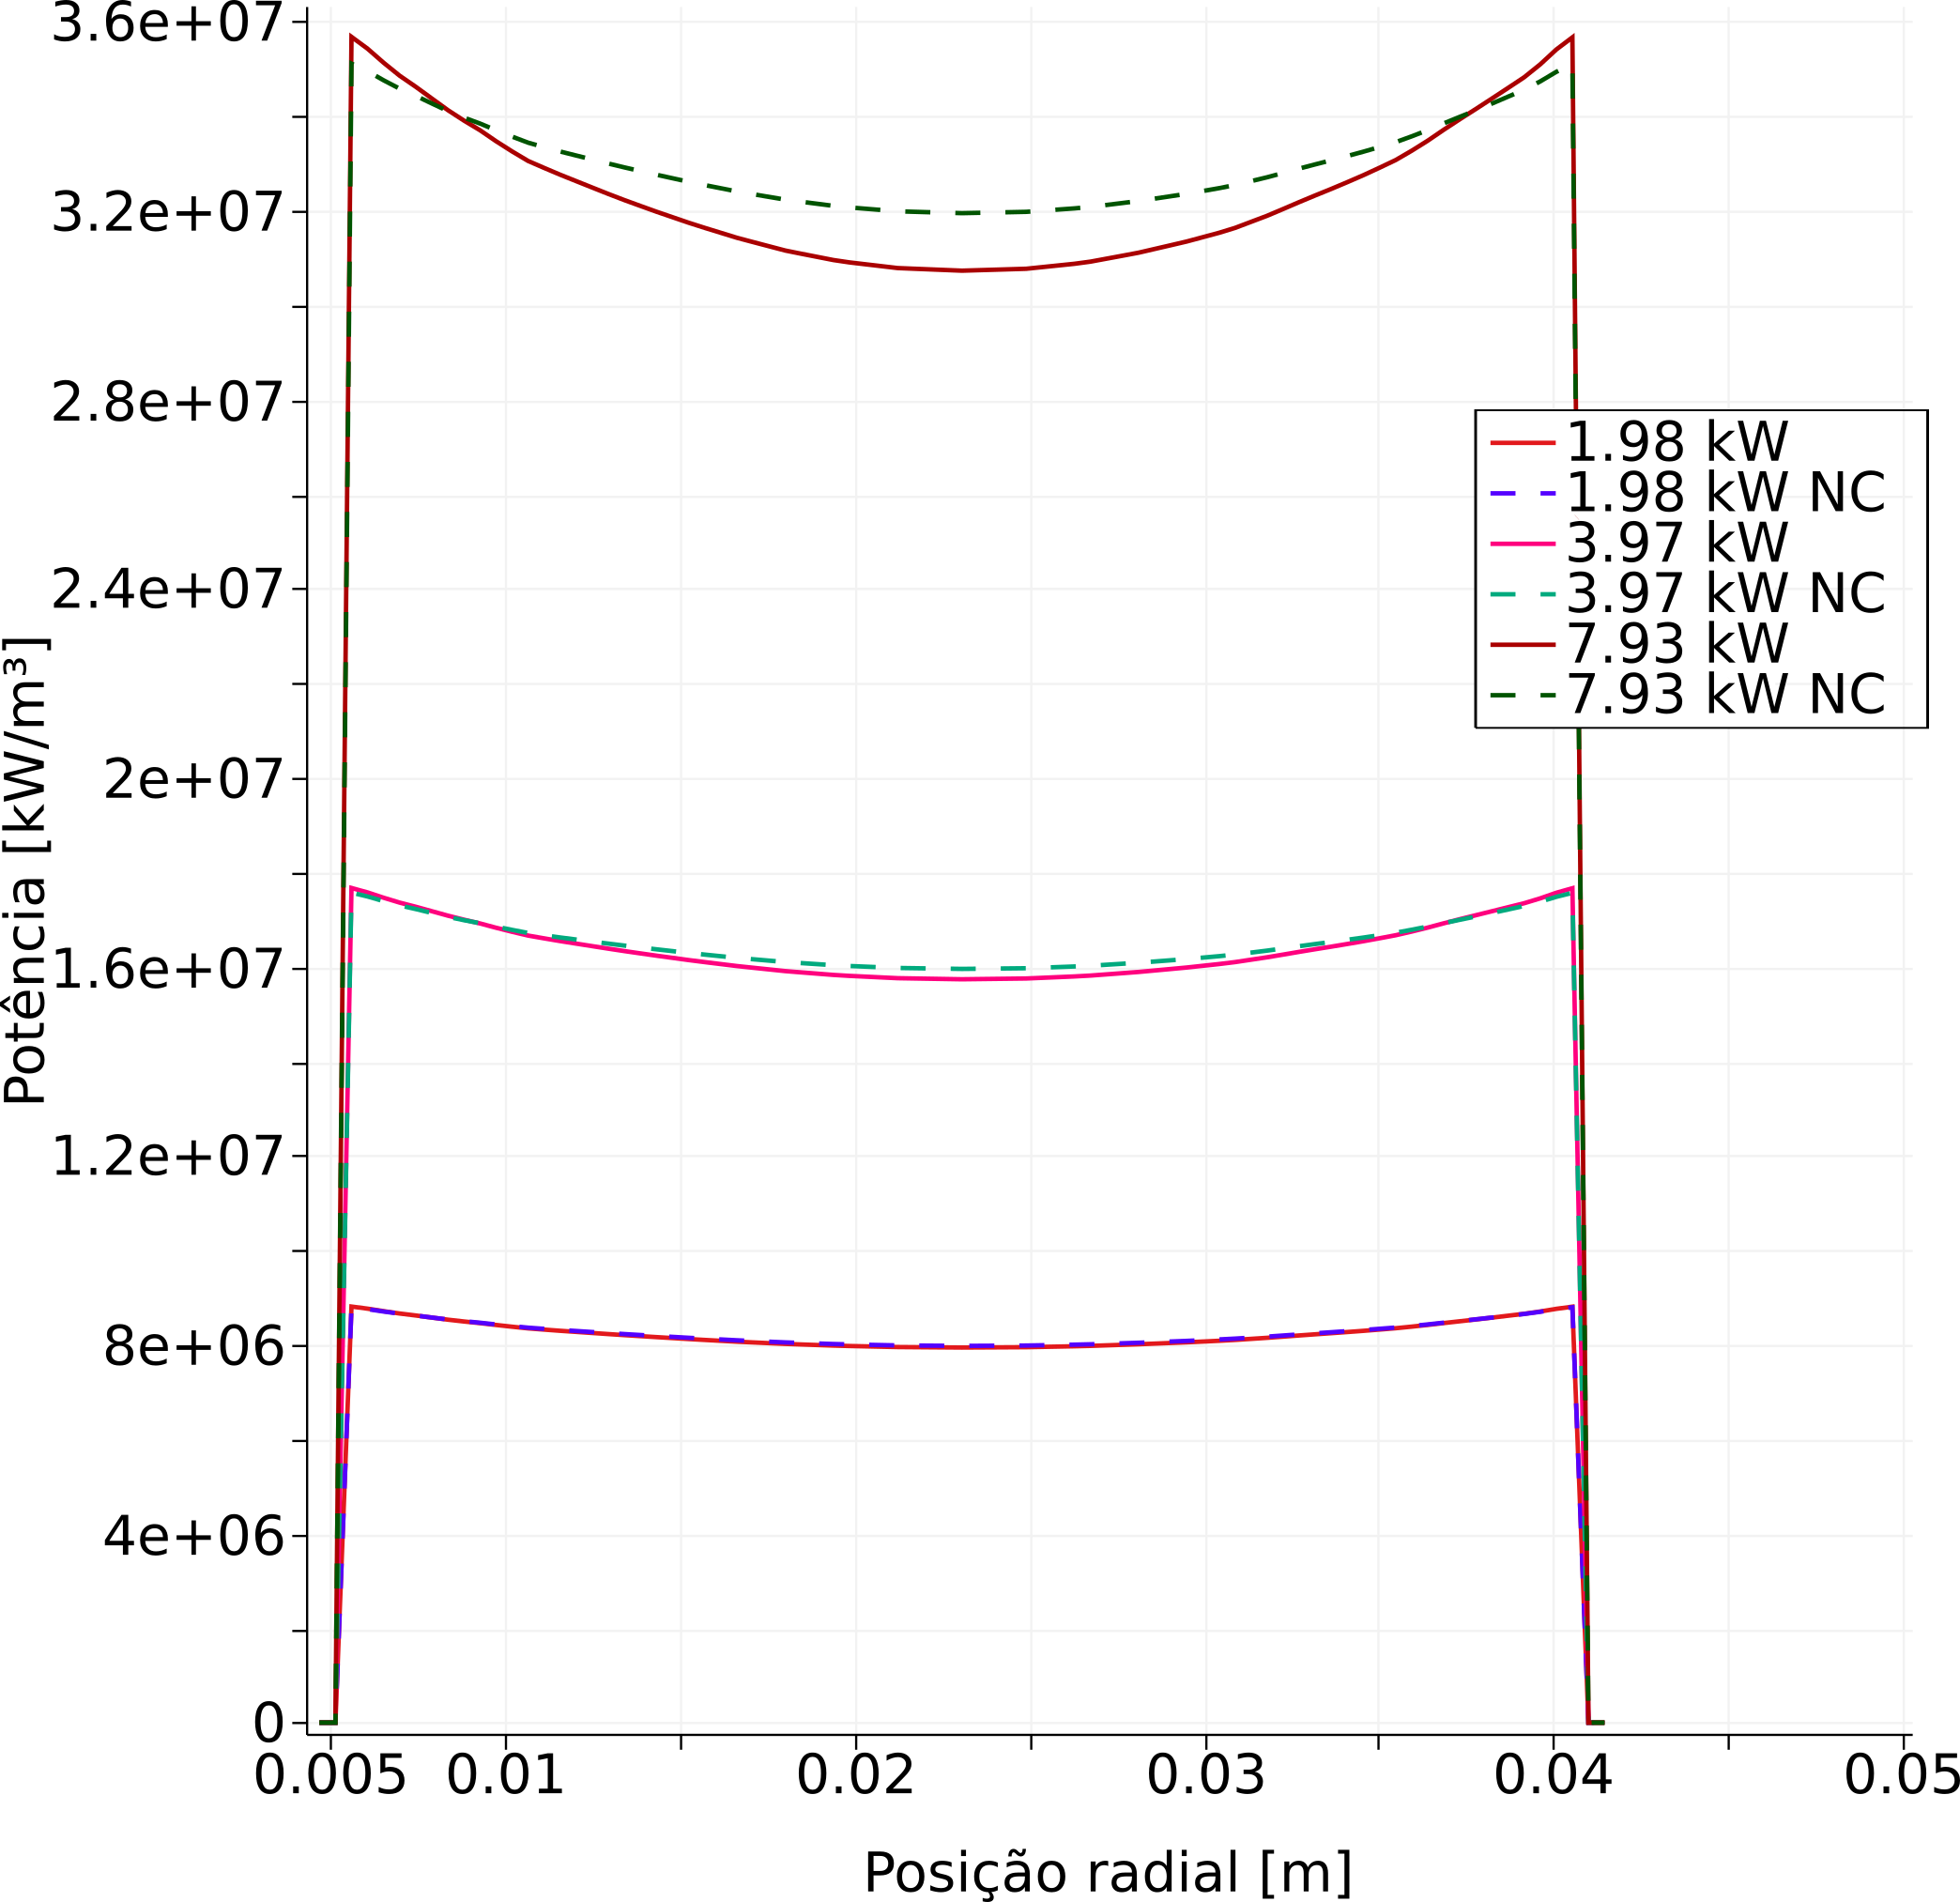
\includegraphics[scale=0.5]{figuras/Q_all_x_square_port.png}
  \label{fig:Q_all_x}
%  \legend{Fonte: autor}
\end{figure}
  


% ----------------------------------------------------------
% Conclusões
% ----------------------------------------------------------
% ----------------------------------------------------------
% Conclusões
% ----------------------------------------------------------
\chapter{Conclusões}
\label{chap:conclusoes}

Nesta tese foi desenvolvido um sistema livre, aberto e gratuito para
cálculos neutrônicos e termo-hidráulicos de forma acoplada utilizando
malhas idênticas. Além do sistema propriamente dito, foi também desenvolvida
uma metodologia para a construção deste sistema acoplado baseada em sistemas
já existentes livres e utilizando memória compartilhada como forma de
intercâmbio de dados.

Este sistema é inovador ao utilizar o \textit{framework OpenFOAM}, baseado
em volumes finitos, como ferramenta de cálculos termo-hidráulicos e o
código de cálculos de física de reatores aberto \textit{milonga} como ferramenta
para cálculos neutrônicos. A utilização de memória compartilhada como
espaço de intercâmbio de dados, apesar de conhecida \cite{Maciel2011, Theler2013},
é praticamente ignorada pela comunidade de Engenharia Nuclear Computacional na
implementação de sistemas acoplados. Tal situação é de se estranhar, já que o
uso de memória compartilhada permite a comunicação entre os sistemas acoplados
de forma confiável, robusta e tão rápida quanto qualquer acesso à memória
do computador. O sistema desenvolvido nesta tese faz uso de memória compartilhada,
sendo o único sistema conhecido de cálculos acoplados baseados em volumes finitos. 

O sistema desenvolvido, por acoplar dois sistemas de cálculos que utilizam
a formulação de volumes finitos para solução de sistemas de equações diferenciais,
explora a característica de domínio idêntico para os dois sistemas. Em outras palavras,
os domínios de solução, ou malhas, são os mesmos para ambos o que evita a utilização
de funções de mapeamento, ou seja, evita o \textit{overhead} do mapeamento geométrico,
um problema de geometria computacional não-trivial no caso de malhas não-estruturadas.

Há, naturalmente, vantagens e desvantagens no uso de malha idêntica. Uma desvantagem
é o custo computacional para malhas refinadas. Além disso, o fluxo neutrônico geralmente
não precisa ser conhecido em detalhes na maioria dos cálculos de núcleo de reatores,
o que fundamenta eventuais críticas ao custo computacional do sistema desenvolvido. 
Entretanto, o objetivo dos cálculos por volumes
finitos é permitir identificar pequenas ocorrências imperceptíveis
em cálculos por métodos menos granulares. O sistema desenvolvido nesta tese, cuja
prova conceitual foi feita com uma malha relativamente pobre, permite conhecer fenômenos
locais calculados a partir de elementos da multi-física envolvida, e não apenas
de perfis de potência genéricos ou temperaturas médias, por exemplo. 

O desenvolvimento desta tese levou também a contribuições fora do seu escopo principal.
Incidentalmente, ao acessar o código-fonte dos sistemas utilizados para permitir seu
uso acoplado, foram encontradas
falhas de implementação em ambos os sistemas utilizados para neutrônica e termo-hidráulica.
Os erros encontrados no \textit{OpenFOAM} foram reportados à comunidade.
Os erros encontrados no \textit{milonga} não só foram reportados ao seu autor como,
em um caso crítico, foi feita a correção diretamente e então enviado o \textit{patch} ao autor.
Essa correção foi incorporada numa versão posterior do \textit{milonga}.
Estas contribuições incidentais se dão devido à própria natureza do desenvolvimento baseado
em \textit{software} livre, que prevê e se baseia em contribuições e trocas entre a comunidade
de usuários, desenvolvedores e autores.

É dessa corrente de desenvolvimento que surge outra característica inovadora
do sistema desenvolvido nesta tese: ele é construído exclusivamente a partir
de sistemas abertos e livres\footnote{A metodologia utilizada
  na geração de seções de choque utiliza um \textit{software} restrito. Entretanto, a geração
  de seções de choque, apesar de fundamental para os cálculos neutrônicos, não é, propriamente dita,
  parte do sistema acoplado, já que qualquer ferramenta pode ser utilizada para este propósito. Neste tema, começam também a surgir opções em \textit{software} livre
  visando a geração de seções de choque em multi-grupos a partir de bibliotecas contínuas \cite{Slaybaugh2014}.}.
Esta característica e suas implicações merecem uma seção exclusiva.


\section{Discussão sobre \textit{software} livre}

A princípio, o fato de um \textit{software} ser distribuído de forma livre ou restrita pode soar indiferente.
Entretanto, numa avaliação mais cuidadosa, é fácil
perceber que a liberdade na utilização, modificação e distribuição de um \textit{software} trás imediatamente
diversos benefícios ao seu usuário. O primeiro
benefício é financeiro. Não é necessário dispender dinheiro em licenças de uso, autorizações de uso ou
qualquer outro aspecto do uso de \textit{software}. Essa independência financeira na relação com o \textit{software} é, em último caso,
ainda mais importante para países em desenvolvimento que, nem sempre, conseguem garantir um fluxo constante
no aporte de financiamento a instituições de pesquisa e acadêmicas. O Brasil entra, obviamente, nesta lista.

A liberdade de utilização está intimamente ligada ao acesso ao código-fonte, que, como anteriormente apresentado,
é obrigatoriamente distribuído com a versão binária ou executável do \textit{software} no caso de sistemas
livres. A capacidade de estudar, entender, modificar e experimentar
com o \textit{software} está totalmente ligada ao acesso a como se dá seu funcionamento. É novamente fácil perceber que,
do ponto de vista tecnológico, o acesso ao código-fonte funciona como uma transferência de tecnologia. Além disso, no
aspecto educacional, é uma forma de colocar as novas e futuras gerações de profissionais em contato com a tecnologia na
prática, para além das abordagens didáticas e teóricas, por vezes limitadas a casos canônicos ou simplificações. 


%\begin{figure}[htb]
%  \caption{Conclusões: o sistema acoplado.}
%  \centering\includegraphics[scale=0.7]{figuras/conclusoes1.png}
%  \label{metodoetapas}
%  \legend{Fonte: autor}
%\end{figure}

Complementando os aspectos financeiro e de liberdade de utilização, há ainda, no tocante ao \textit{software} livre,
o aspecto de distribuição do conhecimento. Se não explicitamente, já que um código sem comentários e sem manual oferece
pouca oportunidade de aprendizado se tomarmos o pior caso, um código medianamente comentado e com um manual de utilização mesmo
simples oferece uma oportunidade para se conhecer novas técnicas de desenvolvimento, linguagens, padrões de desenvolvimento, ferramentas,
métodos e algoritmos. E esta lista é não-exaustiva. Além disso, baseada nas contribuições comunitárias, a lista de possibilidades
de aprendizado cresce de acordo com o número de contribuintes e a intensidade com que contribuem. Deve-se ainda mencionar
a autoverificação. Um código aberto é amplamente auditável e, quanto mais usuários o leem, maior a possibilidade de se
encontrar falhas ou, em alguns casos, código malicioso. Talvez seja este aspecto, o alicerce que sustenta a forma de desenvolvimento
livre. E aparentemente, essa forma de desenvolvimento, ainda que de forma tardia, começa a atingir a indústria nuclear
\cite{Romano2013, Boyd2014, Theler2014b, Huff2016}.


Cabe, antes de finalizar esta seção, uma observação. Não se pretende nesta breve discussão advogar em favor do \textit{software}
livre como a solução mágica para todos os problemas do conhecimento humano. Há uma infinidade de situações em que pode ser desejável
que detalhes de implementação ou que o código-fonte seja preservado, por exemplo. A razão pode ser financeira, estratégica ou de segurança.
O que se pretende, não sem certa ousadia, é trazer à luz a discussão do uso e desenvolvimento de \textit{software} livre na e pela indústria nuclear. Há sólidos
argumentos favoráveis e contrários à sua utilização. O que não se pode é ignorar sua existência e abrir mão de investigar e discutir como
esta filosofia, se se pode utilizar esta palavra, de desenvolvimento de Sistemas de Computação pode vir a contribuir no desenvolvimento
da Engenharia Nuclear.

\section{Trabalhos Futuros}

Em um trabalho de prova de conceito, a discussão sobre perspectivas futuras ganha uma importância adicional.
O sistema desenvolvido nesta tese possui diversas limitações, apresentadas na seção \ref{subsec:lim}. Uma vez
provado o conceito, o próximo passo consiste em estender o alcance do sistema a casos mais complexos. Para
isso devem ser superadas as limitações técnicas apresentadas. Além disso, sendo o sistema acoplado nada
mais do que ambos os sistemas utilizados modificados internamente, eventuais melhorias no sistema acoplado
passam, obrigatoriamente, por evolução, modificações ou expansão nos sistemas utilizados. Sendo assim, nesta seção são apresentadas formas
de superar as limitações já apresentadas bem como opções adicionais com o objetivo de ampliar a utilização
do sistema acoplado atual. 

Hoje, tanto o \textit{OpenFOAM} quanto o \textit{milonga} são distribuídos exclusivamente para o sistema
operacional Linux \cite{LinuxBritannica}. Para fazer com que sejam utilizados em outras plataformas, são necessárias
modificações em seus códigos-fonte e em seus sistemas de compilação e instalação. O \textit{OpenFOAM}, dada sua
ampla rede de usuários, já possui iniciativas neste sentido. O \textit{milonga}, entretanto, possui apenas pequenas partes
adaptadas à compilação multiplataforma. De forma a expandir o alcance de ambos, é necessário fazer com que ambos
sejam passíveis de compilação multiplataforma. Há, disponíveis, ferramentas com esse intuito \cite{Martin2008}. Com ambos os
sistemas funcionais em multiplataforma, as modificações no sistema acoplado seriam pequenas e factíveis.

Um trabalho futuro que traria enormes impactos na capacidade de atacar grandes problemas em relação malhas refinadas
com muitos elementos é a implementação de uma versão paralela do \textit{milonga}. A implementação em paralelo dos
cálculos em volumes finitos e de cálculo das matrizes do problema de autovalores permitira uma escalabilidade
fundamental para os cálculos neutrônicos. Na versão atual, todo o processo é feito sequencialmente: toda a malha
é percorrida, todas as interpolações célula a célula feitas, então é construída a matriz de solução e então resolvido
o sistema na matriz. A execução em paralelo permite dividir o domínio em cada núcleo\footnote{A arquitetura dos processadores
  atuais implementa unidades de processamento independentes, denominadas \textit{core}. Isso significa que a
capacidade de multiprocessamento é inerente a esses processadores.} e resolver paralelamente
uma escala menor do problema. Isso se aplica tanto ao problema de construção das matrizes a partir dos volumes finitos
quanto à solução da matriz propriamente dita. Algoritmos de solução de matrizes de vários tipos, amplamente conhecidos
e utilizados, estão disponíveis sendo, alguns dos mais robustos deles \cite{Hernandez2005, Balay2016}, distribuídos livremente.
Neste caso, seriam necessárias adaptações no sistema acoplado dependendo da forma de divisão do domínio. Estas adaptações teriam
um certo grau de complexidade. Entretanto, a implementação do sistema acoplado já foi feita com vistas à execução em paralelo,
de modo que laços e elementos de programação paralela estão implementados para distintos núcleos utilizando MPI \cite{Quinn2004}.

De carona na implementação em paralelo, outra candidata a melhorias é a função de percurso de células atualmente
implementada no \textit{milonga}. Levantamentos preliminares mostraram que a atual implementação do \textit{milonga}
gasta grande parte do tempo de execução nesta função, devido à interpolação de temperaturas por célula. A otimização
desta função levaria a ganhos no tempo total de execução. A otimização desta função não está diretamente ligada à
implementação em paralelo. Entretanto, antes da paralelização de qualquer algoritmo, é usual que
se trabalhe na sua versão ótima (ou tão boa quanto possível).

A aplicação utilizada para a prova de conceito se restringiu à utilização da aproximação por difusão para os cálculos
de fluxo de nêutrons. O \textit{milonga} oferece ainda a opção de utilização do método de ordenadas discretas,
também chamado de método $S_N$ \cite{Hebert2009}, para a solução da equação de transporte. Entretanto, para problemas
maiores a demanda por memória do método citado inviabiliza seu uso. A reimplementação deste método com objetivo de
otimizar o uso de memória pode ser um caminho para a solução mais precisa do fluxo de nêutrons se comparado ao método
de aproximação por difusão. Além disso, está em curso a implementação do método de características \cite{Hebert2009} no \textit{milonga}
por membros da comunidade argentina de Física de Reatores.

A expansão do \textit{solver OpenFOAM} para o cálculo de transientes além de estado estacionário também é possível.
Para isso, uma abordagem é adaptar um novo \textit{solver OpenFOAM} já existente capaz de lidar com variações em relação
ao tempo utilizando os arquivos e modificações já feitas no sistema atual. Este seria um trabalho mais elaborado.

Outra linha de trabalho consiste em alterar a utilização de malhas em ambos os códigos, otimizando o uso de memória
compartilhada. Neste caso, as classes utilizadas no \textit{OpenFOAM} na implementação da utilização de malhas podem
ser estendidas - servindo-se do conceito de herança existente no paradigma de programação orientada a objetos e
no qual o \textit{OpenFOAM} se baseia - para que o armazenamento de toda a estrutura de dados se dê em memória compartilhada.
Isso exigiria ainda que toda a implementação do \textit{milonga} no tratamento de malhas, fosse também modificada de acordo.
Esta abordagem já consiste num grande trabalho de projeto e implementação de software. A consequência deste trabalho seria
a utilização de uma única macroestrutura de dados para representação do domínio em memória, utilizando, a grosso modo,
metade da memória utilizada na implementação atual. Essa nova implementação poderia, ainda, ser projetada para
funcionar em paralelo.

Ainda no tocante à implementação dos sistemas envolvidos, há a possibilidade de utilizar a capacidade ociosa de placas
gráficas para, por exemplo, a solução das matrizes de autovalores. Esta abordagem, entretanto, necessita de mais estudos
sobre sua viabilidade.

Fora dos trabalhos futuros relativos à implementações de novas funcionalidades, estão simulações numéricas mais elaboradas
utilizando-se o sistema atual. É fato que, com as limitações atuais, em especial relativas ao cálculo sequencial, não é
possível utilizar o sistema para problemas elaborados. Porém, estudos de validação utilizando problemas conhecidos
(\textit{benchmarks}) são fundamentais para que o sistema desenvolvido possa ser, eventualmente, considerado para
simulações em nível de licenciamento ou aplicações de missão crítica.

Os possíveis caminhos de desenvolvimento futuro e aplicações não estão limitados aos apresentados neste capítulo.
A expectativa ao fim deste trabalho de tese é continuar contribuindo para o desenvolvimento do ecossistema de
ferramentas computacionais com foco nas vantagens do desenvolvimento baseado em \textit{software} livre para todos
os envolvidos e interessados em Computação Científica aplicada à Engenharia Nuclear.




% ----------------------------------------------------------
% ELEMENTOS PÓS-TEXTUAIS
% ----------------------------------------------------------
\postextual


% ----------------------------------------------------------
% Referências bibliográficas
% ----------------------------------------------------------
\bibliography{tese}

% ----------------------------------------------------------
% Glossário
% ----------------------------------------------------------
%
% Consulte o manual da classe abntex2 para orientações sobre o glossário.
%
%\glossary

% ----------------------------------------------------------
% Apêndices
% ----------------------------------------------------------

% ---
% Inicia os apêndices
% ---
%\begin{apendicesenv}

% Imprime uma página indicando o início dos apêndices
%\partapendices

% ----------------------------------------------------------
% ----------------------------------------------------------

%\end{apendicesenv}
% ---


% ----------------------------------------------------------
% Anexos
% ----------------------------------------------------------

% ---
% Inicia os anexos
% ---

%\begin{anexosenv}

%% Imprime uma página indicando o início dos anexos
%\partanexos

%\chapter{Simulação de subcanais do reator TRIGA IPR-R1}
%\label{ane:INAC2013}
%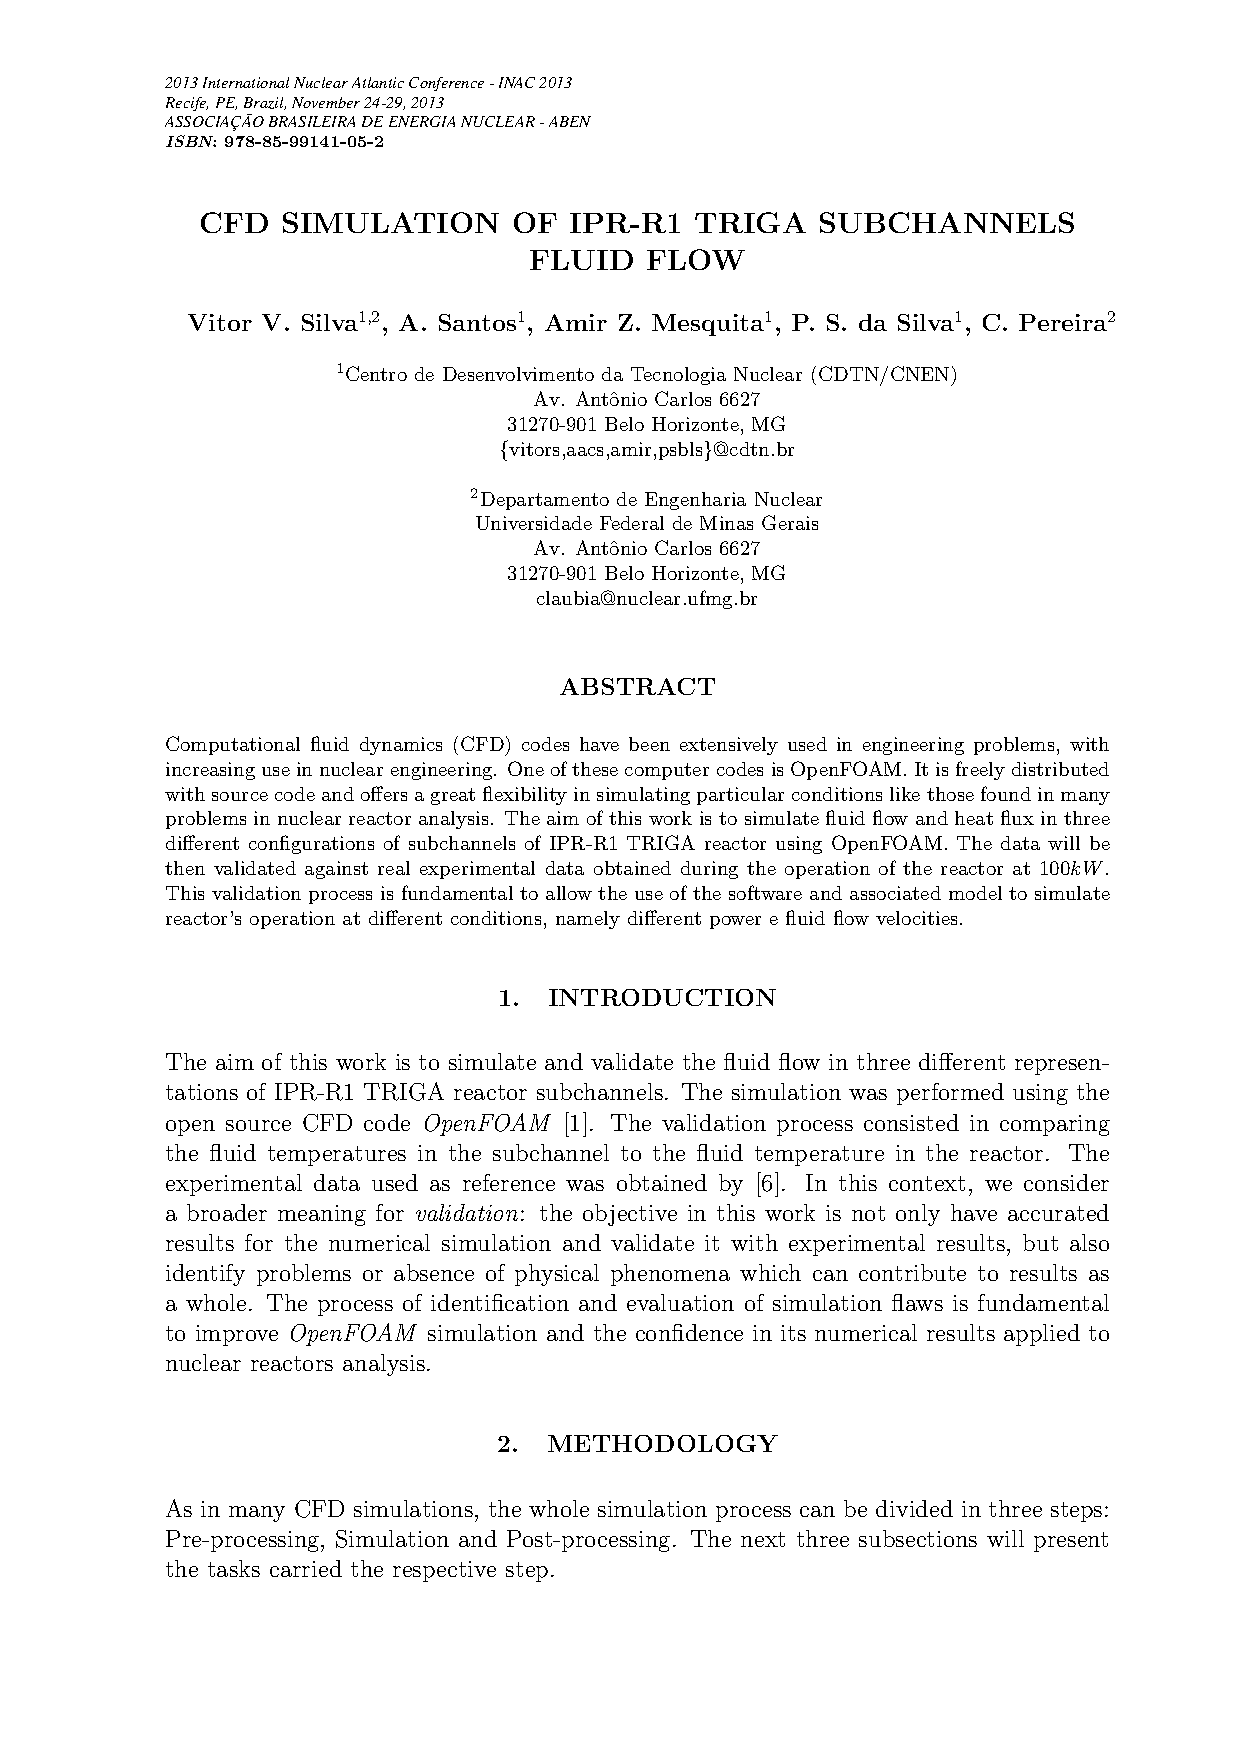
\includepdf[pages={-}]{anexos/inac2013.pdf}

%\chapter{Simulação do combustível do reator TRIGA IPR-R1 com 
%ANSYS/CFX}
%\label{ane:simfuel}


%\chapter{Paper RRFM 2013}
%\label{ane:RRFM2013}
%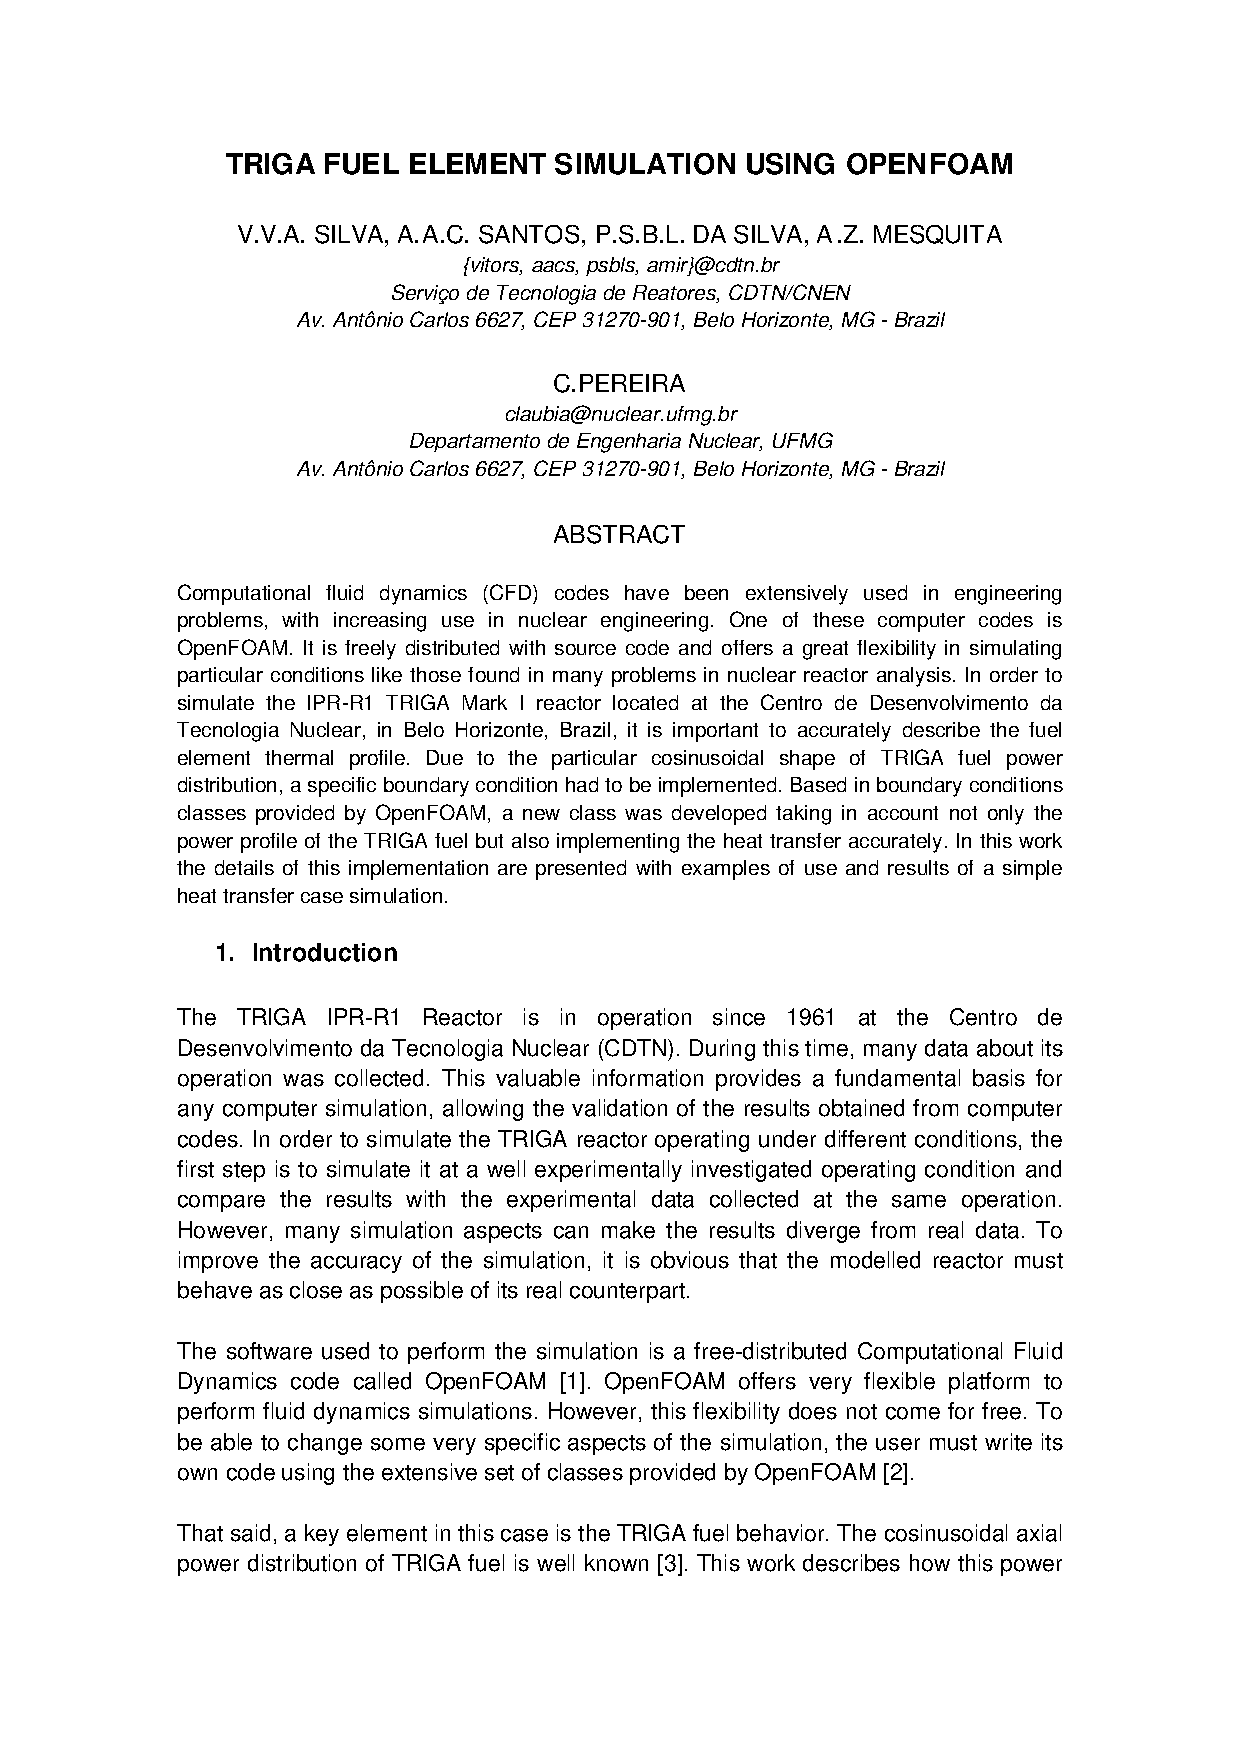
\includepdf[pages={-}]{anexos/RRFM2013}


%\chapter{Pedido do registro de Produto Tecnológico INPI}
%\label{ane:trigafuel}
%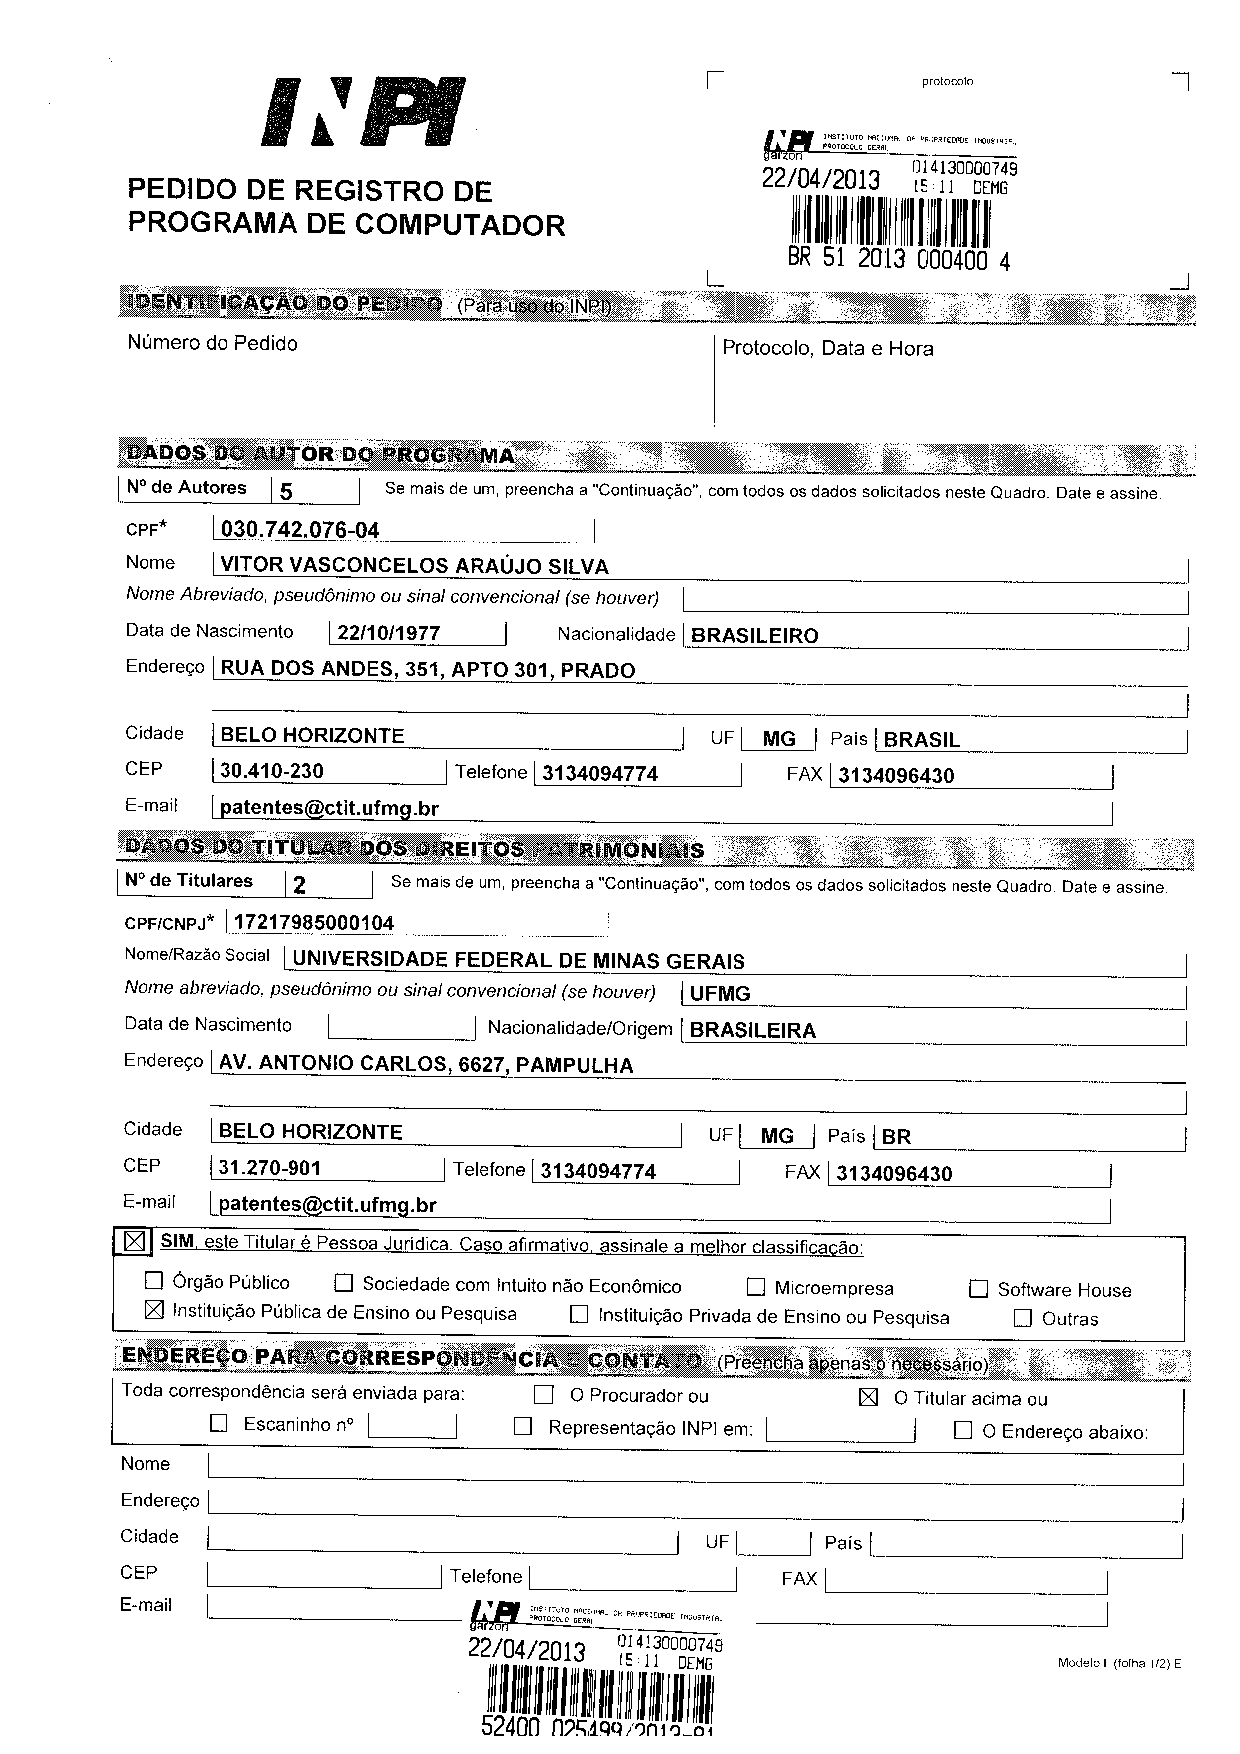
\includepdf[pages={-}]{anexos/depositotrigafuel.pdf}

%\end{anexosenv}

%---------------------------------------------------------------------
% INDICE REMISSIVO
%---------------------------------------------------------------------

\printindex

\end{document}
